\documentclass[a4paper,12pt,oneside]{article}
\usepackage[utf8]{vietnam}
\usepackage{graphicx}
\graphicspath{ {figures/} }
\usepackage{fancyhdr}
\usepackage{geometry}
\usepackage{array}
\usepackage{float}
\usepackage{morefloats}
\usepackage[bottom]{footmisc}
\usepackage{afterpage}
\usepackage{makecell}
\usepackage{multirow}
\usepackage{pdflscape}
\usepackage[table]{xcolor}
\usepackage{indentfirst}%thut dau dong doan moi
\usepackage[unicode]{hyperref}%tao bookmark
\hypersetup{urlcolor=blue,linkcolor=black,citecolor=black,colorlinks=true}
\usepackage{commath}
\usepackage{amsmath}
\usepackage{listings,xcolor}
\usepackage{amssymb}

\DeclareMathOperator*{\argmin}{arg\,min}
%\usepackage[pdftex,bookmarks,raiselinks,pageanchor,hyperindex,colorlinks]{hyperref}
\definecolor{highlight}{RGB}{230, 230, 230}
\newcommand{\kb}{\textit{KB/s}}
\newcommand{\kbs}{\textit{Kbps}}
\newcommand{\mbs}{\textit{Mbps}}
\newcommand{\gbs}{\textit{Gbps}}
\newcommand{\mb}{\textit{MB/s}}
\newcommand\blankpage{%
\null
\thispagestyle{empty}%
\addtocounter{page}{-1}%
\newpage}
\geometry{
left=3cm, right=2cm,
top=2cm, bottom=2cm,
includefoot=true,
includehead=true
}
% create the header for this file
\pagestyle{fancy}

\usepackage{textcomp}
\usepackage{tabularx}
\usepackage{setspace}
\usepackage{tikz}
\usetikzlibrary{fit}
\usetikzlibrary{arrows,automata}
\usetikzlibrary{arrows,shapes,positioning,shadows,trees}
\usepackage{booktabs}
\setlength{\heavyrulewidth}{1.5pt}
\setlength{\abovetopsep}{4pt}

\usetikzlibrary{positioning,arrows.meta,spy}

\definecolor{arrowblue}{RGB}{98,145,224}

\newcommand\ImageNode[3][]{
\node[draw=arrowblue!80!black,line width=1pt,#1] (#2) {\includegraphics[width=3cm,height=3cm]{#3}};
}
\renewcommand {\baselinestretch}{1.5}

\usepackage{eso-pic}
\newcommand\BackgroundPic{%
\put(15,0){%
\parbox[b][\paperheight]{\paperwidth}{%
\vfill
\centering

\includegraphics[width=0.8\paperwidth,height=0.9\paperheight]{hinh/background.jpg}%
\vfill
}}}

\usepackage[nottoc]{tocbibind}

\pagenumbering{roman}

\begin{document}
\thispagestyle{empty}
\AddToShipoutPicture*{\BackgroundPic}

\begin{center}
\begin{large}
\textbf{ĐẠI HỌC QUỐC GIA THÀNH PHỐ HỒ CHÍ MINH}
\end{large} \\
\begin{large}
\textbf{TRƯỜNG ĐẠI HỌC BÁCH KHOA}
\end{large} \\
\begin{large}
\textbf{KHOA KHOA HỌC \& KỸ THUẬT MÁY TÍNH}
\end{large} \\
\textbf{-----------------------------------------}\\[1cm]
\begin{center}

\includegraphics[scale=.1]{hinh/logo.png}\\[1cm]
\end{center}


{\fontsize{15pt}{1}\selectfont \textbf{LUẬN VĂN TỐT NGHIỆP ĐẠI HỌC}}\\[1.75cm]

\begin{spacing}{2}
{\fontsize{18pt}{1}\selectfont \textbf{PHÁT TRIỂN BOARD ĐIỀU KHIỂN VÀ\\
HỆ THỐNG HỖ TRỢ NÔNG NGHIỆP ĐÔ THỊ}}\\
\end{spacing}
\end{center}

{\fontsize{13pt}{1}
\begin{tabbing}

\hspace*{5cm} \= \textbf{HỘI ĐỒNG:} \hspace*{0.01cm} \= \textbf{Công nghệ phần mềm} \\
\> \textbf{GVHD:} \> \textbf{ThS. Nguyễn Cao Trí}\\
\> \textbf{GVPB:} \> \textbf{ThS. Lê Đình Thuận}\\
\> -----------------------------------------------------------------------------\\
\> \textbf{SVTH 1:} \> \textbf{Huỳnh Bá Thạch} \hspace*{1cm} \= \textbf{(51303742)}\\
\> \textbf{SVTH 2:} \> \textbf{Tạ Chí Tây} \> \textbf{(51303574)}\\
\> \textbf{SVTH 3:} \> \textbf{Nguyễn Đình Dũng} \> \textbf{(51300665)}\\
\> \textbf{SVTH 4:} \> \textbf{Nguyễn Lê Minh Khôi} \> \textbf{(51301906)}\\
\end{tabbing}
}

\vspace{\fill}
\begin{center}
{\fontsize{20pt}{1} TP Hồ Chí Minh, 01/2018}\\
\end{center}
\ClearShipoutPicture

\newpage

\begin{center}
{\fontsize{20pt}{1}\selectfont \textbf{LỜI CAM ĐOAN}}\\[1cm]
\end{center}
Nhóm xin cam đoan đây là công trình thực hiện của nhóm và được sự hướng dẫn của ThS. Nguyễn Cao Trí. Ngoài các thông tin thu thập được có ghi rõ nguồn trong phần Tài liệu, các phần thiết kế và hiện thực khác đều do chính nhóm thực hiện và chưa được công bố trước đây. Nhóm xin hoàn toàn chịu trách nhiệm về mặt nội dung luận văn tốt nghiệp của mình. Trường đại học Bách Khoa – Đại Học
Quốc Gia Thành Phố Hồ Chí Minh không liên quan đến những vi phạm tác quyền,
bản quyền do nhóm gây ra trong quá trình thực hiện (nếu có).
\begin{flushright}
Nhóm thực hiện đề tài
\end{flushright}

\newpage
\begin{center}
{\fontsize{20pt}{1}\selectfont \textbf{LỜI CẢM ƠN}}\\[1cm]
\end{center}
\noindent Lời đầu tiên, chúng tôi xin được gửi lời cảm ơn chân thành đến ThS. Nguyễn Cao Trí – người thầy đã cho chúng tôi cơ hội được tham gia nghiên cứu và hiện thực đề tài này. Trong quá trình hiện thực, thầy đã thường xuyên trao đổi và hỗ trợ về mặt kiến thức, ý tưởng, tài liệu và kinh phí để nhóm có thể hoàn thiện được đề tài từ giai đoạn thực tập tốt nghiệp đến giai đoạn luận văn tốt nghiệp. \\
\noindent Nhóm cũng xin gửi lời cảm ơn đến các thầy cô trường Đại Học Bách Khoa – Đại Học Quốc Gia Thành phố Hồ Chí Minh nói chung và các thầy cô trong khoa Khoa Học và Kỹ Thuật Máy Tính nói riêng, đã truyền đạt những kiến thức quý báu, làm nền tảng cho quá trình thực hiện đề tài.
Xin gửi lời cảm ơn chân thành đến gia đình, bạn bè, những người đã luôn hỗ trợ và động viên chúng tôi trong quá trình thực hiện luận văn tốt nghiệp. \\
\noindent Báo cáo được thực hiện trong khoảng ba tuần, không thể tránh khỏi những sai sót, nhóm rất mong được sự đóng góp của các thầy cô để nhóm có thể hoàn thiện hơn.\\
\noindent Sau cùng, nhóm xin kính chúc các thầy cô trường Đại Học Bách Khoa – Đại Học Quốc Gia Thành phố Hồ Chí Minh luôn dồi dào sức khỏe để có thể tiếp tục trên con đường truyền đạt kiến thức cho các thế hệ sinh viên.

\begin{flushright}
Nhóm thực hiện đề tài
\end{flushright}
% %%%%%%%%%%%%_ MUC LUC_%%%%%%%%%%%%%%%
\newpage
\begin{center}
{\fontsize{20pt}{1}\selectfont \textbf{TÓM TẮT}}\\[1cm]
\end{center}
Sự phát triển của công nghệ trong thời đại hiện nay đã  mang lại nhiều thay đổi tích cực trong tất cả các lĩnh vực. Và lĩnh vực nông nghiệp cũng có những bước tiến lớn trong thời đại của cuộc cách mạng công nghiệp 4.0. Hòa cùng với xu thế của thời đại, sinh viên nhóm chúng tôi đã tìm hiểu và thực hiện dự án về hệ thống công nghệ hỗ trợ dành cho nông nghiệp, đặc biệt đối với nông nghiệp trong đô thị. Sự phát triển mạnh mẽ của Internet of Things và sự cần thiết của nó dành cho nông nghiệp trong môi trường đô thị, nơi mà không có nhiều không gian dành cho nông nghiệp, đã được thực hiện ở giai đoạn Thực tập tốt nghiệp, đề tài tiếp tục được phát triển ở giai đoạn Luận văn tốt nghiệp. Tại giai đoạn này, nhóm tiếp tục xây dựng hệ thống hoàn chỉnh hơn từ hình mẫu đã được thiết kế và xây dựng từ giai đoạn trước, đầy đủ hơn các chứng năng cơ bản để hỗ trợ giám sát và chăm sóc cho một hệ thống thủy canh trong môi trường đô thị. Hệ thống bao gồm phần cứng và phần mềm trên nền tảng ứng dụng web và ứng dụng di động được cải thiện về mặt giao diện, tương tác thân thiện hơn với người dùng và cung cấp các API hữu ích cho những nhà phát triển.

\newpage
\tableofcontents

\newpage
\listoffigures

\newpage
\listoftables

\newpage
\section*{Danh sách chữ viết tắt}
\label{sec:dsvt}
\addcontentsline{toc}{section}{\nameref{sec:dsvt}}

\begin{enumerate}
\item \textbf{IoT} Internet of Things
\item \textbf{RFID} Radio Frequency Identification
\item \textbf{NFC} Near Field Communication
\item \textbf{IP} Internet Protocol
\item \textbf{API} Application Programming Interface
\item \textbf{CSDL} Cơ Sở Dữ Liệu
\item \textbf{HTML} Hypertext Markup Language
\item \textbf{MVC} Model - Controller - View
\item \textbf{SPA} Single Page Application
\item \textbf{UI} User Interface
\item \textbf{IDE} Integrated Development
 Environment
 \item \textbf{CRUD} Create, Read, Update, Delete
\end{enumerate}

\newpage
\pagenumbering{arabic}
\section{GIỚI THIỆU ĐỀ TÀI}

\subsection{Ý tưởng}

\noindent Công nghệ thủy canh đã được nghiên cứu từ thế kỷ 17. Đến nay, công nghệ này đã hoàn thiện và hướng tới việc sản xuất ra những sản phẩm nông nghiệp sạch. Công nghệ thủy canh có thể áp dụng với quy mô lớn trong các nông trại hoặc với quy mô nhỏ trong các hộ gia đình. Nhóm đang hướng tới đối tượng là các hộ gia đình ở thành phố, nơi diện tích chật hẹp và không có đất để trồng trọt. Họ có thể tận dụng các khoảng không nhỏ trong nhà như sân thượng, lan can,… để đặt một giàn thủy canh nhỏ với năng suất cao, cung cấp nguồn nông sản sạch cho gia đình. Đồng thời hướng đến việc tự động hóa các công việc chăm sóc, người dùng không phải mất nhiều thời gian để chăm sóc cho cây trồng nhưng chúng vẫn có thể tự phát triển và cho năng suất cao.

\noindent Trên thế giới hiện đã có những ứng dụng sử dụng IoT để tự động hóa hoàn toàn quy trình trồng rau sạch thủy canh nhà phố, trong khi ở Việt Nam còn khá mới mẻ. Với những yếu tố trên, nhóm đã hiện thực và phát triển hệ thống hỗ trợ cho mô hình thủy canh theo hướng kết hợp IoT với mục đích giúp người dùng tạo ra nông sản sạch, không ô nhiễm.


\subsection{Mục tiêu}
\subsubsection{Phần nghiên cứu}
\begin{itemize}
\item Tìm hiểu và thực hành quá trình thiết kế và xây dựng một dự án.
\item Tìm hiểu nắm vững các nên tảng, thư viện cũng như các công cụ để thực hiện dự án này.
\item Áp dụng các kiến thức về thiết kế mềm, kĩ thuật lập trình vào dự án.
\item Tổ chức dự án cho phép dễ dàng bảo trì, mở rộng.
\item Tìm hiểu về hệ thống các mô hình thủy canh: 
	\begin{itemize}
	\item Tổng quan, khái niệm về thủy canh.
	\item Các mô hình thủy canh và cách vận hành của từng mô hình.
	\end{itemize}
\item Học hỏi và biết cách sử dụng các công nghệ mới hiện nay như Nodejs, Angularjs, Angular 2, Ionic, ...
\end{itemize}

\subsubsection{Phần kết quả}

\begin{itemize}
\item Hiện thực mạch đo giá trị ppm (parts per million) trong môi trường dung dịch.
\item Hệ thống board điều khiển với các cảm biến (nhiệt độ, độ ẩm, ánh sáng, ppm) và các relay điều khiển (máy bơm nước, quạt, đèn) có thể đáp ứng các tiêu chí:
	\begin{itemize}
		\item Vận hành trong thời gian dài, ổn định.
		\item Chức năng thu thập dữ liệu các cảm biển phải hoạt động tốt, ổn định, sai số chấp nhận được.
		\item Chức năng điều khiển các thiết bị như máy bơm nước, sục oxi, đèn chiếu sáng.. đáp ứng thời gian thực.
		\item Các kết nối về sóng wifi ổn định, cung cấp chức năng cấu hình cho module wifi.
		\item Protocol giao tiếp giữa board điều khiển và web-server hoạt động chính xác.
		\item Thiết kế hiện thực board điều khiển về mặt phần cứng, phần khung, vỏ bảo vệ.
	\end{itemize} 
\item Xây dựng website cho người dùng với các chức năng:
	\begin{itemize}
		\item Thu nhận các thông tin từ thiết bị  gửi lên từ các cảm biến.
		\item Phân tích các thông tin gửi lên, giám sát, đưa ra cảnh báo và giải pháp xử lý đối với trường hợp các thông tin vượt ngưỡng cho phép.
		\item Tạo một lịch trình và nạp xuống cho thiết bị.
		\item Theo dõi thường xuyên, upload hình ảnh về các mùa vụ đang trồng.
		\item Chia sẻ thông tin của mình cho các người dùng khác, xây dựng một cộng đồng chung để mọi người trao đổi và chia sẻ thông tin trong lĩnh vực thủy canh.
	\end{itemize}
\item Hiện thực mô hình thủy canh thu nhỏ cho demo.
\end{itemize}


\newpage

\section{CƠ SỞ LÝ THUYẾT}

\subsection{Giới thiệu về Internet of Things}

\subsubsection{Internet of Things (IoT)}

\noindent Internet of Things - "Mạng lưới vạn vật kết nối Internet là một kịch bản của thế giới, khi mà mỗi đồ vật, con người được cung cấp một định danh của riêng mình, và tất cả có khả năng truyền tải, trao đổi thông tin, dữ liệu qua một mạng duy nhất mà không cần đến sự tương tác trực tiếp giữa người với người, hay người với máy tính"\cite{iot}. Tất cả mọi thứ được kết nối với nhau qua mạng Internet, người dùng có thể quản lý mọi thiết bị thông qua mạng bằng các thiết bị như PC, smartphone, tablet...Các thiết bị sẽ giao tiếp với nhau, hạn chế sự tác động của con người. Sự giao tiếp chủ yếu là việc thu thập, xử lý thông tin từ các thiết bị rồi tự đưa ra quyết định, hành động phù hợp với những thông tin thu thập được. Với sự phát triển của các thiết bị thông minh ngày càng gia tăng thì IoT được xem như tương lai của thế giới.

\noindent Chúng ta có thể hình dung rằng mọi thiết bị trong hệ thống kết nối, hoạt động cùng với nhau. Khi ta bước gần về đến cửa nhà, cơ chế điều khiển sẽ tự động mở cửa từ xa, đèn cửa và hành lang được kích hoạt. Hệ thống điều hòa đang từ trạng thái chờ sẽ chuyển sang trạng thái hoạt động. Mọi thứ điều hoạt động một cách tự động, hài hòa nhờ sự kết nối với nhau thông qua mạng Internet. Đó chính là những gì IoT mang lại cho chúng ta.

\begin{figure}[H]
\centering
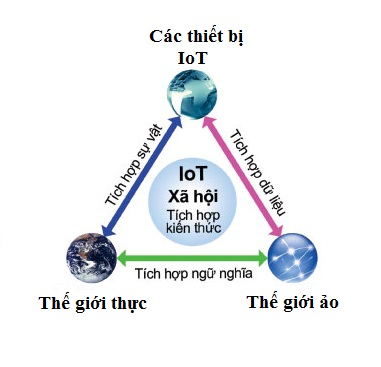
\includegraphics[scale=.7]{hinh/IoT_intro.jpg}
\caption{Mô hình tương tác của mạng lưới thiết bị kết nối Internet\cite{iot}.}
\end{figure}

\subsubsection{Định danh}

\noindent "Điểm quan trọng của IoT đó là các đối tượng phải có thể được nhận biết và định dạng (identifiable)"\cite{iot}. Trong môi trường Internet việc truyền nhận thông tin cần thiết nhất là địa chỉ IP. Hiện tại địa chỉ IP phổ biến thường dùng là IPv4 (mỗi địa chỉ có 32 bit). Với sự phát triển và tăng nhanh về mặt số lượng của các thiết bị thông minh kết nối với Internet làm cho địa chỉ IPv4 ngày càng ít. Sự xuất hiện của địa chỉ IPv6 (mỗi địa chỉ có 128 bit) đã giải quyết vấn đề về việc định danh cho cái thiết bị tham gia vào mạng Internet. 

\noindent Khi mọi đối tượng được định danh sẽ làm cho việc quản lý các đối tượng trong mạng IoT trở nên dễ dàng hơn.

\subsubsection{Cấu trúc của hệ thống IoT\cite{cautruciot}}

\noindent \textbf{Cảm biến}\\
\noindent Các cảm biến có chức năng thu thập các tín hiệu analog từ môi trường thông qua việc quét các thông số sang tín hiệu digital.

\noindent \textbf{Xử lý cục bộ và lưu trữ}\\
\noindent Dữ liệu được lưu trữ và xử lý cục bộ thông qua các vi điều khiển, board mạch nhúng. Xử lý các tín hiệu thông tin nhận được từ cảm biến. Các thiết bị phần cứng có khả năng giao tiếp theo các quy tắc đã được định sẵn. Chúng rất đa dạng tùy vào mục đích sử dụng.

\noindent Vi điều khiển là những thiết bị nhỏ, dễ dàng kết nối, có thể lập trình, nhiều mã nguồn mở đơn giản. Tuy nhiên vì có kích thước nhỏ nên khả năng, tốc độ xử lý không cao, RAM chỉ khoảng 2KB đối với Arduino. Chúng không chạy hệ điều hành, phần mềm chạy trên đó được gọi là Firmware, giống như một chương trình. Đối với loại máy tính mini như Raspberry Pi có thể chạy hệ điều hành đồng nghĩa với việc sức mạnh và tốc độ xử lý cao hơn, mạnh mẽ hơn.

\noindent Có nhiều thiết bị được phát triển dành cho công nghệ IoT, tùy nhu cầu mà chọn thiết bị cho phù hợp với mục đích, chi phí sử dụng. Một số thiết bị như: STM32, ARM, Arduino, ChipKIT, v.v...

\noindent \textbf{Network và Internet}\\
\noindent Các thiết bị phần cứng thu thập dữ liệu cục bộ và đẩy dữ liệu lên cloud để lưu trữ. Những giao thức giao tiếp giữa thiết bị phần cứng và cloud thường được sử dụng ở tầng này:
\begin{itemize}
	\item CoAP (Constrained Application Protocol)
	\item MQTT (Message Queuing Telemetry Transport)
	\item HTTP (HyperText Transfer Protocol)
	\item XMPP (Extensible Messaging and Presence Protocol)
\end{itemize}

\noindent \textbf{Cloud (đám mây)}\\
\noindent Nơi dữ liệu được thu thập, bao gồm hệ thống các máy chủ, hệ thống lưu trữ.

\subsubsection{Ứng dụng}

\noindent IoT có ứng dụng vô cùng rộng, trong rất nhiều lĩnh vực, có thể kể ra một số ứng dụng nổi bật hiện nay như sau:
\begin{itemize}
\item Nhà thông minh.
\item Thành phố thông minh.
\item Xe hơi tự hành.
\item Vườn tự chăm sóc.
\item Máy bay không người lái.
\item Thiết bị theo dõi sức khỏe.
\item Hệ thống chiếu sáng tự động.
\item Chuỗi cung ứng thông minh.
\end{itemize}

\begin{figure}[H]
	\centering
	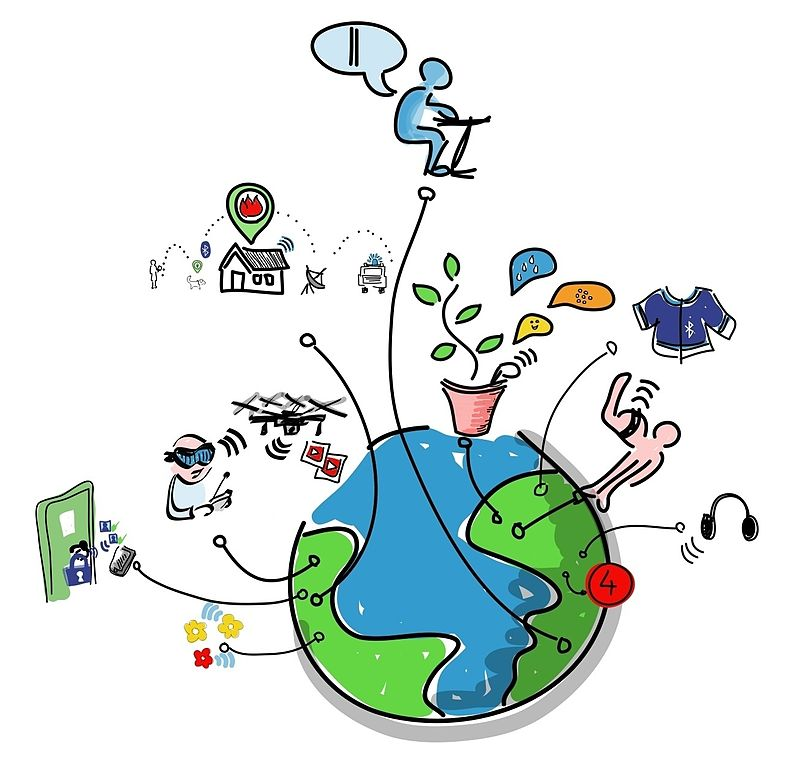
\includegraphics[scale=.4]{hinh/IoT_ungdung.jpg}
	\caption{Cả thế giới chìm trong Internet\cite{iot}.}
	\label{fig:IoT_ungdung}
\end{figure}

\subsection{Giới thiệu về hệ thống thủy canh\cite{thuycanh}}

\noindent Thủy canh là một kỹ thuật trồng cây trong môi trường dung dịch dinh dưỡng, có thể hiểu là trồng cây trong nước, do có rất nhiều môi trường tổng hợp được sử dụng để trồng cây nên có thể định nghĩa thủy canh là "Trồng cây không sử dụng đất"\cite{thuycanh}, thay vào đó rễ được giữ trong các giá thể như xơ dừa, trấu, sỏi nhẹ, mút xốp… Đây là phương pháp dùng nước làm môi trường cung cấp đầy đủ các chất dinh dưỡng cần thiết cho sự phát triễn của cây. Ngoài ra vẫn đảm bảo các yếu tố như ánh sáng cho quá trình quang hợp, oxi cho quá trình hô hấp để cây phát triển tốt, năng suất cao. 

\noindent Đối với phương pháp thủy canh có thể điều chỉnh nồng độ dinh dưỡng ít hay nhiều tùy vào từng giai đoạn phát triển của cây một cách nhanh chóng. Thủy canh thích hợp cho các khu vực có diện tích nhỏ hẹp, chật chội như sân thượng, ban công nhà cửa thành phố… Quá trình đô thị hóa, dân số ngày càng tăng, diện tích đất đai bị thu hẹp thì kỹ thuật thủy canh sẽ mang lại lợi ích to lớn cho đời sống, hơn thế nữa kỹ thuật này không gây ô nhiễm môi trường, tạo ra nông sản sạch, giúp chất lượng cuộc sống nâng cao.

\subsubsection{Hệ thống dạng bấc (Wick System)}
\noindent Hệ thống dạng bấc là dạng hệ thống đơn giản nhất, đây là hệ thống bị động. “Đặt một đầu của sợi bấc hút sao cho chạm vào phần rễ cây. Đầu kia của bấc chìm trong dung dịch dinh dưỡng”\cite{thuycanh}. Dung dịch dinh dưỡng và nước sẽ được hút thông qua các sợi bấc.

\begin{figure}[H]
	\centering
	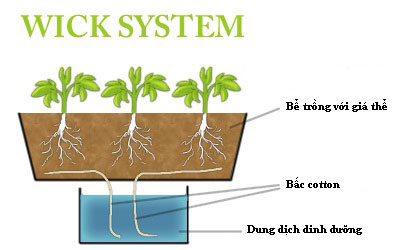
\includegraphics[scale=.8]{hinh/Wick_system.jpg}
	\caption{Mô hình hệ thống dạng bấc\cite{thuycanh}.}
	\label{fig:Wick_system}
\end{figure}

\subsubsection{Hệ thống thủy canh tĩnh (Water Culture)}
\noindent Hệ thống thủy canh tĩnh gồm thùng nước chứa dung dịch dinh dưỡng, ”phần bệ giữ cây thường làm bằng chất dẻo nhẹ như xốp và đặt nổi ngay trên dung dịch dinh dưỡng”\cite{thuycanh}. Dùng máy bơm cung cấp khí và khối sủi bọt dung dịch dinh dưỡng, cung cấp oxy cho rễ cây. Hệ thống này thường được dùng phổ biến trong môi trường giảng dạy vì ít tốn kém, có thể tận dụng các vật chứa nước hoặc những bình chứa không rỉ khác.

\begin{figure}[H]
	\centering
	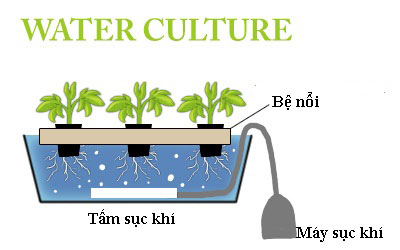
\includegraphics[scale=.8]{hinh/Water_culture.jpg}
	\caption{Mô hình hệ thống thủy canh tĩnh\cite{thuycanh}.}
	\label{fig:Water_culture}
\end{figure}

\subsubsection{Hệ thống ngập và rút định kỳ (EBB and Flow System)}

\noindent Hệ thống ngập và rút định kì hoạt động bằng cách làm khay trồng ngập trong dung dịch dinh dưỡng trong một khoảng thời gian, sau đó rút dung dịch này trở lại vào bồn chứa. Hoạt động được thực hiện bởi máy bơm có kết nối với bộ đếm thời gian bật tắt máy bơm để dung dịch vào khay và trở lại bồn chứa theo chu kì. Tùy thuộc vào từng loại cây mà sẽ có chu kì ngập rút dài ngắn khác nhau.

\begin{figure}[H]
	\centering
	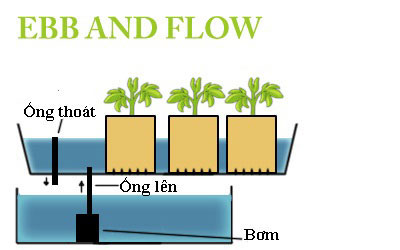
\includegraphics[scale=.9]{hinh/ebb_flow.jpg}
	\caption{Mô hình hệ thống ngập và rút định kỳ\cite{thuycanh}.}
	\label{fig:ebb_flow}
\end{figure}

\subsubsection{Hệ thống nhỏ giọt (Drip System)}
\noindent Hệ thống nhỏ giọt là hệ thống hoạt động bằng cách dùng máy bơm dung dịch lên nhỏ giọt trực tiếp vào các giá thể thông qua các đường ống dẫn, sau đó dung dịch dinh dưỡng dư sau khi thấm qua các giá thể sẽ quay trở lại vào bể chứa để chuẩn bị được bơm lên lần kế tiếp. Quá trình này được tiếp diễn liên tục. Hệ thống này hoạt động khá hiểu quả dựa vào việc tái sử dụng dung dịch dinh dưỡng dư, không bị lãng phí.

\begin{figure}[H]
	\centering
	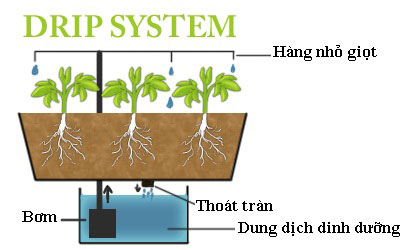
\includegraphics[scale=.9]{hinh/Drip_system.jpg}
	\caption{Mô hình hệ thống nhỏ giọt\cite{thuycanh}.}
	\label{fig:Drip_system}
\end{figure}


\subsubsection{Hệ thống màng dinh dưỡng NFT (Nutrient Film Technique)}
\noindent Hệ thống màng dinh dưỡng NFT là hệ thống hoạt động bằng việc dùng máy bơm liên tục dung dịch dinh dưỡng vào khay trồng để chảy qua rễ rồi trở lại bể chứa, quá trình này được diễn ra liên tục. Đối với kỹ thuật này thì thường không sử dụng thêm giá thể, giúp tiết kiệm về mặt chi phí giá thể.


\begin{figure}[H]
	\centering
	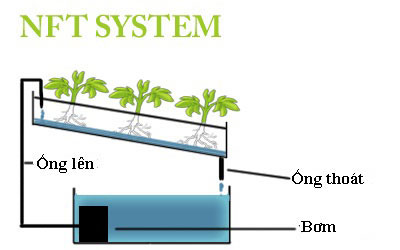
\includegraphics[scale=.8]{hinh/NFT_system.jpg}
	\caption{Mô hình hệ thống màng dinh dưỡng NFT\cite{thuycanh}.}
	\label{fig:NFT_system}
\end{figure}


\subsubsection{Khí canh (Aeroponics)}

\noindent Hệ thống khí canh hoạt động bằng cách phun sương dung dịch dinh dưỡng vào rễ cây được phơi trong không khí. Quá trình tạo sương được thực hiện định kì mỗi vài phút. Đối với kỹ thuật này cây được cung cấp đầy đủ dinh dưỡng, nước và không khí. "Hiện nay khí canh thường được ứng dụng trong mô hình trồng khoai tây."\cite{thuycanh}


\begin{figure}[H]
	\centering
	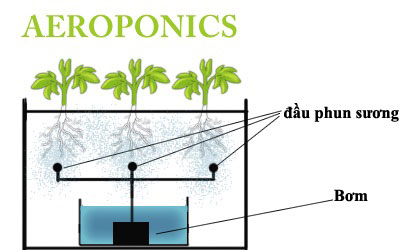
\includegraphics[scale=.9]{hinh/aeroponics.jpg}
	\caption{Mô hình hệ thống khí canh\cite{thuycanh}.}
	\label{fig:aeroponics}
\end{figure}


\subsubsection{Các thông số trong dung dịch thủy canh, thiết bị đo ppm}

\begin{itemize}
\item Độ dẫn điện EC (electro-conductivity) (tương đối) là "chỉ số diễn tả tổng nồng độ ion hòa tan trong dung dịch. Độ dẫn điện có thể được thể hiện bằng một số đơn vị khác nhau, nhưng đơn vị tiêu biểu được dùng để đo lường EC là millisiemens trên centimet (mS / cm)"\cite{ec}. Chỉ số EC không diễn tả nồng độ của từng chất trong dung dịch đồng thời cũng không thể hiện mức độ cân bằng của các chất dinh dưỡng trong dung dịch. EC là thước đo độ dẫn điện từ hai đầu dò 1cm.\\
Trong suốt quá trình tăng trưởng, cây hấp thu khoáng chất mà chúng cần, do vậy duy trì EC ở một mức ổn định là rất quan trọng. Nếu dung dịch có chỉ số EC cao thì sự hấp thu nước của cây diễn ra nhanh hơn sự hấp thu khoáng chất. Điều này làm nồng độ dung dịch tăng cao và gây ngộ độc cho cây. Khi đó ta phải bổ sung thêm nước vào môi trường. Ngược lại, nếu EC thấp, cây sẽ hấp thu khoáng chất nhanh hơn hấp thu nước. Khi đó, nồng độ dung dịch giảm mạnh, cây sẽ không được cung cấp đầy đủ khoáng chất, chậm lớn và phát triển kém.

\item Chỉ số TDS (Total Dissolved Solids) là "chỉ số đo tổng lượng chất rắn hoà tan, tổng số các ion mang điện tích bao gồm khoáng chất, muối hoặc kim loại tồn tại trong một khối lượng nước nhất định. TDS thường được biểu thị bằng hàm số ml/L hoặc ppm (Parts Per Million). 1 ppm tương ứng với 1mg chất rắn hòa tan trong một lít nước. Hầu hết nước máy sẽ có chỉ số PPM rơi vào khoảng từ 200 – 400ppm"\cite{ec}. Chỉ số TDS cũng ảnh hưởng lớn đến sự phát triển của cây: Nếu TDS lên quá cao, nồng độ dung dịch vượt mức cho phép sẽ gây ra hiện tượng ngộ độc cho cây. Ngược lại, khi chỉ số TDS xuống thấp, dung dịch thủy canh sẽ không đảm bảo cung cấp đủ chất dinh dưỡng cho cây trồng.

\item Tương quan giữa EC và TDS: mặc dù có một mối tuơng quan giữa EC và TDS nhưng chúng không giống nhau. TDS và EC là 2 tham số riêng biệt. TDS là tổng lượng chất rắn hoà tan trong nước. EC là khả năng của các chất co thể gây ra dòng điện. Lượng chất rắn như muối trong phân bón tỉ lệ trực tiếp với độ dẫn điện của nó, vì vậy lượng chất rắn cao gây độ dẫn cao. Vì khi phân bón hoà tan trong nước chúng trở thành các "ion", có mang điện tích âm hoặc dương, nên chúng sinh ra dòng điện.\\
Mối quan hệ của TDS và độ dẫn đặc hiệu của nước ngầm có thể được ước lượng bằng phương trình sau:
\begin{center}
		TDS = ke*EC
\end{center}					
Trong đó: TDS có đơn vị mg\/L và EC là độ dẫn điện ở microsiemens trên mỗi centimet ở 25\textdegree{}C. Yếu tố tương quan ke dao động từ 0,55 đến 0,8.\\
Giới hạn với cây trồng:
\begin{figure}[H]
	\centering
	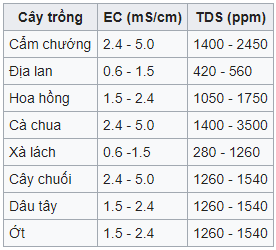
\includegraphics[scale=.8]{hinh/PPM/ppm_thamkhao.PNG}
	\caption{Giới hạn với cây trồng\cite{ec}.}
	\label{fig:ppm_thamkhao}
\end{figure}

\item Tại sao lại dùng thiết bị này?\\
Nếu EC / PPM chỉ là đo điện dẫn (hoặc kháng) thì tại sao không sử dụng một đồng hồ volt / ohm trực tiếp? Bởi chúng đi qua dòng điện DC thông qua các đầu dò và bạn không thể đo độ dẫn của muối với dòng điện DC vì nó sẽ tách các phân tử ra ngoài, và vì các phân tử là điện dẫn điện, các phần tử điện sẽ thay đổi liên tục và sẽ không thu được kết quả gì. Bằng cách sử dụng một tín hiệu AC,với tần số đủ cao (> 1khz) các phân tử không có thời gian để di chuyển ra ngoài trước khi chúng được kéo theo hướng ngược lại.\\
Các thành phần ion:
\begin{figure}[H]
	\centering
	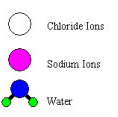
\includegraphics[scale=1]{hinh/PPM/ppm_ion.png}
	\caption{Các thành phần ion\cite{ppm}.}
	\label{fig:/ppm_ion}
\end{figure}

Trường hợp sử dụng dòng AC:
\begin{figure}[H]
	\centering
	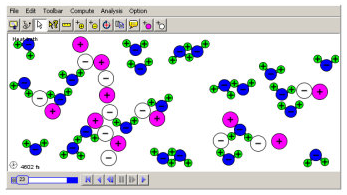
\includegraphics[scale=1]{hinh/PPM/ppm_AC.png}
	\caption{Trường hợp sử dụng dòng AC\cite{ppm}.}
	\label{fig:ppm_AC}
\end{figure}

Trường hợp sử dụng dòng DC:
\begin{figure}[H]
	\centering
	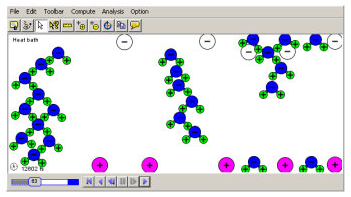
\includegraphics[scale=1]{hinh/PPM/ppm_DC.png}
	\caption{Trường hợp sử dụng dòng DC\cite{ppm}.}
	\label{fig:ppm_DC}
\end{figure}

\item Hoạt động: hai điện cực với một điện áp xoay chiều được đặt trong dung dịch. Điều này tạo ra một dòng điện phù thuộc vào bản chất dẫn điện của dung dịch. Thiết bị đọc dòng diện này và hiển thị theo đơn vị EC hoặc ppm.
\end{itemize}

\subsection{Hệ thống thủy canh với IoT}
\noindent Việc kết hợp thủy canh và IoT ở nước ngoài đã trở nên khá phổ biến trong khi ở Việt Nam vẫn còn mới mẻ. Việc kết hợp IoT vào thủy canh giúp người sử dụng mô hình có thể kiểm soát một cách dễ dàng tình trạng của vườn trồng thủy canh thông qua số liệu về nhiệt độ, độ ẩm, pH, v.v... mà các cảm biến gửi về qua mạng Internet. Đồng thời người dùng có thể chăm sóc vườn rau của mình mà không cần thiết phải tiếp xúc với nó nhờ các hoạt động như tưới nước, bơm oxy, cung cấp ánh sáng, quạt, v.v... đều được thiết lập theo lịch trình thông qua các ứng dụng. Người dùng chỉ việc thiết lập thông số lịch trình phù hợp cho từng cây trồng trong mỗi mùa vụ và chờ ngày thu hoạch. Kiểm soát thông qua mạng Internet cho phép người dùng quản lý vườn trồng của mình ở bất kỳ đâu, trong mọi thời điểm.  Chính vì vậy mà thủy canh kết hợp với IoT là xu hướng mới và là tương lai của nông nghiệp đô thị nhờ tính tiện ích của nó.

\subsection{Các hệ thống thủy canh tự động hiện có trên thị trường}
\noindent Theo quá trình nghiên cứu của nhóm thì hiện nay trên thị trường chưa có nhiều hệ thống thủy canh tự động mang tính thương mại. Một số công ty start-up nổi tiếng trong lĩnh vực này như Hachi, Lisado nhưng những hệ thống này có các đặc điểm chung:
	\begin{itemize}
		\item Mới chỉ phát triển ở khu vực phía Bắc.
		\item Chỉ hỗ trợ nền tảng di động, chưa hỗ trợ môi trường web trên PC hay laptop.
		\item Chưa có một hệ thống để cộng đồng có thể chia sẻ kinh nghiệm về thủy canh với nhau.
		\item Chưa hỗ trợ tự động đo nồng độ dinh dưỡng ppm.
		\item Chưa hỗ trợ tính năng cài đặt lịch trình tự động cho các hoạt động chăm sóc vườn.
	\end{itemize} 
\noindent Sản phẩm của nhóm đang hướng tới sự khác biệt bằng cách tạo ra một hệ thống hỗ trợ các tính năng nói trên.
\subsection{Giới thiệu về các công nghệ được sử dụng}

\subsubsection{RESTful web service \cite{restful}}
\noindent REST (Representational State Transfer) là một kiến trúc giao tiếp giữa client và server giúp hệ thống server có thể dễ dàng quản lý tài nguyên, được sử dụng nhiều trong việc phát triển các ứng dụng Web Services sử dụng giao thức HTTP.\\
\noindent Một kiến trúc REST thường gồm một server cung cấp các API truy xuất tài nguyên và client truy xuất, chỉnh sửa các tài nguyên đó thông qua giao thức HTTP.\\
Các phương thức HTTP được sử dụng:
\begin{itemize}
\item POST: sử dụng khi tạo một tài nguyên mới.
\item GET: dùng để truy xuất tài nguyên.
\item PUT: cập nhật tài nguyên.
\item DELETE: dùng để xóa bỏ tài nguyên.
\end{itemize}
\textbf{JSON (Javascript Object Notation)}\\
 Trong hệ thống mà nhóm hiện thực sử dụng cấu trúc JSON để trao đổi dữ liệu. "JSON là 1 định dạng hoán vị dữ liệu nhanh. Chúng là cơ sở dựa trên tập hợp của ngôn ngữ lập trình JavaScript, tiêu chuẩn ECMA-262 phiên bản 3 - tháng 12 năm 1999"\cite{json}.\\
 JSON có cấu trúc đơn giản, dễ sử dụng nên hiện nay nó trở nên rất phổ biến. Cấu trúc một JSON bao gồm nhiều cặp tên và giá trị đi kèm với nhau.
 JSON có 5 dạng dữ liệu chính:
\begin{itemize}
	\item Number: dạng số gồm số nguyên và số thực.
	\item String: dạng chuỗi, nội dung được chứa trong cặp dấu nháy kép ( “ ), những ký tự đặt biệt được escape bởi dấu \.Theo chuẩn JSON thì không sử dụng dấu nháy đơn như Javascript để bọc chuỗi.
	\item Boolean: dạng luận lý gồm 2 giá trị là true và false.
	\item Array: dạng mảng, gồm các phần tử phân cách nhau bởi dấu phẩy ( , ) và mảng được bao bởi cặp dấu ( [ ) và ( ] ).
	\item Object: dạng đối tượng, gồm những cặp giá trị đi cùng nhau, mỗi cặp phân cách bởi dấu phẩy ( , ), đối tượng được bao bởi cặp dấu ( { ) và ( } ), cặp giá trị bao gồm tên và giá trị được phân cách bởi dấu hai chấm ( : ).
	\item Null: giá trị null.
\end{itemize}

\begin{figure}[H]
	\centering
	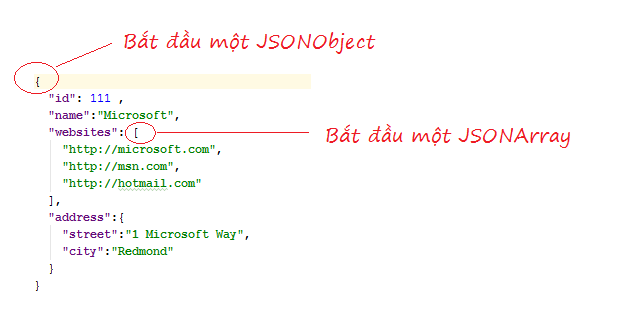
\includegraphics[scale=.8]{hinh/json.png}
	\caption{Cấu trúc một JSON\cite{json}.}
	\label{fig:json}
\end{figure}

Ưu điểm của JSON:
\begin{itemize}
\item Dữ liệu trên nền cơ sở Javascript nên dễ dàng tiếp cận.
\item Dữ liệu truyền tải ngắn gọn.
\item Dễ chuyển đổi (parse) dữ liệu từ dạng chuỗi (nhận từ server) sang dữ liệu có thể sử dụng được (thành Object, Number, Array)…
\item Dễ truy cập nội dung.
\end{itemize}

\subsubsection{Nodejs}
\noindent Nodejs là "một phần mềm mã nguồn mở được viết dựa trên ngôn ngữ JavaScript cho phép lập trình viên có thể xây dựng các ứng dụng chạy trên máy chủ. Phiên bản đầu tiên của Nodejs được cho ra mắt vào năm 2009"\cite{nodejs}.\\
Nodejs là mã nguồn mở, được phát triển trên nhiều nền tảng, chạy trên hệ điều hành như Window, Linux, v.v...  hỗ trợ cung cấp các module đa dạng, giúp phát triển của ứng dụng web một cách đơn giản và dễ dàng.

\begin{figure}[H]
	\centering
	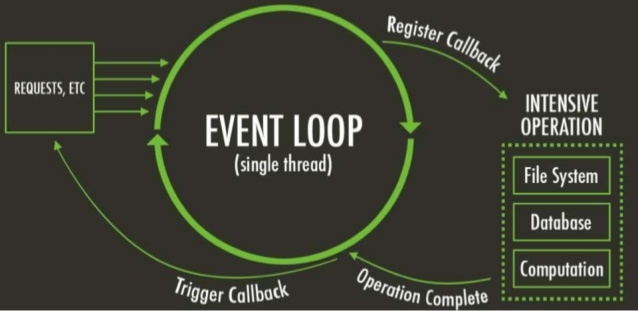
\includegraphics[scale=.8]{hinh/nodejs.png}
	\caption{Cơ chế hoạt động của Nodejs\cite{nodejs}.}
	\label{fig:nodejs}
\end{figure}

\noindent Nodejs đang được sử dụng rộng rãi bởi tốc độ chạy rất nhanh của nó. Sở dĩ Nodejs chạy rất nhanh vì nó thực hiện cơ chế non-blocking I/O và asynchronous (bất đồng bộ). Khi một request đến, nó không dừng lại chờ cho request đó xử lý xong mà vòng lặp event loop sẽ tiếp nhận các request liên tục và xử lý chúng liên tục. Khi một request xử lý xong, hàm callback sẽ được gọi để trả về kết quả cho client hoặc thực hiện một tác vụ nào đó. Như vậy các request sẽ được xử lý song song với nhau, tiết kiệm được rất nhiều thời gian. Nhưng đây cũng là một điểm khó đòi hỏi người lập trình phải quản lý chặt chẽ thứ tự thực hiện các hành động vì không phải lúc nào các tác vụ cũng chạy song song nhau, có những tác vụ phải thực hiện theo tuần tự.

\subsubsection{Framework Expressjs}
\noindent Expressjs là một framework của Nodejs. Expressjs cung cấp cấu trúc đơn giản nhất của một dự án Nodejs (một khung sườn), giúp chúng ta có thể dựa trên đó phát triển một cách nhanh chóng một server RESTful API và có thể dễ dàng từ đó mở rộng nó.

\subsubsection{Sequelizejs}
\noindent Sequelize là một thư viện ORM dành cho Node.js. Nó hỗ trợ truy cập một cách dễ dàng đến PostgreSQL, MySQL, MariaDB, SQLite và MSSQL, v.v...\\
 ORM (Object Relational Mapping) là một kỹ thuật lập trình để ánh xạ dữ liệu giữa các CSDL quan hệ và đối tượng trong các ngôn ngữ lập trình. Trong đó, các đối tượng ánh xạ với các bảng, các quan hệ của đối tượng ánh xạ với các ràng buộc liên quan giữa các bảng. Sequelizejs sẽ giúp chúng ta làm công việc này, nó hỗ trợ các hàm tương ứng thay vì phải viết những câu truy vấn bằng ngôn ngữ SQL. Đây là một module rất tiện lợi cho người lập trình web.
 
\subsubsection{Angularjs}
\noindent Angular là "một bộ Javascript Framework rất mạnh và thường được sử dụng để xây dựng project Single Page Application (SPA)"\cite{angular}.\\
Ưu điểm của Angularjs:
\begin{itemize}
	\item Phát triển dự trên Javascript.
	\item Tạo các ứng dụng client-side theo mô hình MVC.
	\item Khả năng tương thích cao, tự động xử lý mã javascript để phù hợp vứi mỗi trình duyệt.
	\item Mã nguồn mở, miễn phí hoàn toàn và được sủ dụng rộng rãi.
\end{itemize}

\noindent Single page application là một kiểu ứng dụng web mà trong đó, công việc xử lý các thao tác của người dùng đều diễn ra trên một trang duy nhất. Người dùng sẽ có cảm giác trang web hoạt động nhanh hơn do hạn chế tối đa thao tác chuyển trang hoặc tải lại trang.

\subsubsection{Angular 2}
\noindent Angular 2 là một framework để xây dựng các ứng dụng web và ứng dụng di động phía client. Angular 2 ra đời là một bước cải tiến so với Angular 1, nó đưa ra khái niệm "Component", hầu hết các thành phần trong ứng dụng đều quy về Component làm cho ứng dụng trở nên dễ quản lý và dễ phát triển hơn. Angular 2 cũng sử dụng ngôn ngữ Typescript thay vì Javascript như Angular 1. Điều đó có nghĩa là Angular 2 tận dụng được những ưu điểm của ES6 như class, đồng thời giúp cho những người đã quen với các ngôn ngữ kiểu như Java dễ dàng tiếp cận hơn.

\subsubsection{Framework Ionic 2}
\noindent Ionic là "một framework dùng để xây dựng các ứng dụng di động bằng cách sử dụng HTML, CSS, và JavaScript"\cite{ionic}. Nó cho phép gọi các API để tạo ra các ứng dung di động đầy đủ tính năng một cách dễ dàng.
Ionic được xây dựng trên Cordova - framework ứng dụng đa nền tảng cho phép biên dịch ứng dụng thành một tập tin có thể cài đặt và chạy nó bên trong web view của thiết bị di động. Nó cần phải chạy với Angular, xử lý logic của ứng dụng và Cordova, framework ứng dụng đa nền tảng cho phép biên dịch ứng dụng thành một tập tin để cài đặt và chạy trên thiết bị di động. Ứng dụng được xây dựng với Cordova và Ionic có thể chạy trên cả thiết bị Android và iOS.
Điểm cải tiến so với phiên bản 1 là Ionic 2 sử dụng Angular 2 để phát triển các ứng dụng của mình.

\subsubsection{Typescript}
\noindent TypeScript là một dự án mã nguồn mở miễn phí hiện được phát triển và bảo trì bởi Microsoft. "Nó là tập cha của JavaScript, với các bổ sung các tuỳ chọn kiểu tĩnh và lớp trên cơ sở lập trình hướng đối tượng cho ngôn ngữ này"\cite{typescript}. TypeScript có thể sử dụng để phát triển ứng dụng chạy phía client, hay phía server (Node.js). TypeScript là tập cha của JavaScript nên bất kì chương trình JavaScript nào đã có cũng đều là chương trình TypeScript hợp lệ.
  
\subsubsection{JWT}
\noindent JSON Web Token (JWT) là "một tiêu chuẩn mở (RFC 7519) định nghĩa cách thức truyền dữ liệu an toàn giữa các thành phần trong hệ thống thông qua 1 đối tượng JSON. Các dữ liệu này có thể được xác thực độ tin cậy nhờ vào "chữ ký" của nó. Phần chữ ký của JWT sẽ được mã hóa bằng HMAC hoặc RSA"\cite{jwt}.

\begin{figure}[H]
	\centering
	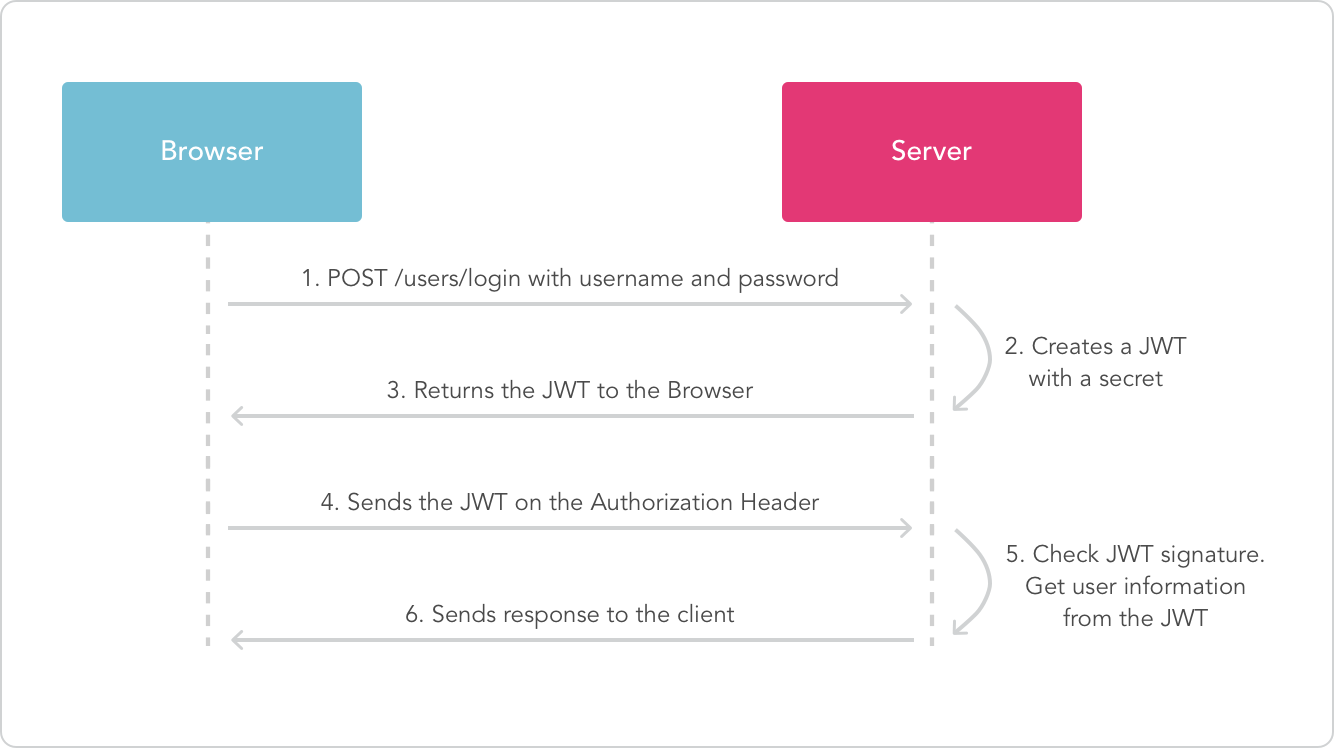
\includegraphics[scale=.35]{hinh/jwt2.png}
	\caption{Quá trình đăng nhập bằng JWT\cite{jwt}.}
	\label{fig:jwt2}
\end{figure}

JWT gồm có 3 phần: 
\begin{itemize}
\item Header\\
Header bao gồm hai phần chính: loại token (mặc định là JWT - Thông tin này cho biết đây là một Token JWT) và thuật toán đã dùng để mã hóa (HMAC SHA256 - HS256 hoặc RSA). 

\begin{center}
\{ "alg": "HS256", "typ": "JWT" \} 
\end{center}

\item Payload\\ 
Payload chứa các claims. Claims là một các biểu thức về một thực thể (chẳng hạn user) và một số metadata phụ trợ. Có 3 loại claims thường gặp trong Payload: reserved, public và private claims. 
\item Signature\\ 
Chữ ký Signature trong JWT là một chuỗi được mã hóa bởi header, payload cùng với một chuỗi bí mật theo nguyên tắc sau: 
\begin{center}
HMACSHA256(  base64UrlEncode(header) + "." +  base64UrlEncode(payload),  secret) 
\end{center}
Do bản thân Signature đã bao gồm cả header và payload nên Signature có thể dùng để kiểm tra tính toàn vẹn của dữ liệu khi truyền tải. 
 
\end{itemize}

\subsubsection{Postgresql}
\noindent PostgreSQL là một hệ quản trị cơ sở dữ liệu quan hệ. Hệ quản trị cơ sở dữ liệu này đã được kiểm chứng và được sử dụng rộng rãi nhờ độ an toàn dữ liệu, đúng đắn, bảo mật. Nó có thể chạy trên các hệ điều hành khác nhau như Linux, Unix, Window. \\
Với việc tuân thủ các tiêu chuẩn của hệ quản trị cơ sở dữ liệu, nó có các tính năng phức tạp như kiểm soát truy cập đồng thời nhiều phiên bản, sao chép không đồng bộ, khôi phục dữ liệu tại từng thời điểm\cite{sql}.

\subsubsection{NodeBB}
\noindent NodeBB là một nền tảng diễn đàn mã nguồn mở thế hệ mới. NodeBB có nhiều tính năng hiện đại và có một cộng đồng hỗ trợ phát triển khá lớn, hỗ trợ xây dựng lên diễn đàn một cách nhanh chóng. Nhóm đã sử dụng framework NodeBB để xây dựng diễn đàn kết hợp với ứng dụng web để tạo nơi trao đổi thông tin cho người dùng trong hệ thống. 

\subsubsection{Git}
\noindent Git là một hệ thống quản lý những tập tin trên máy tính, các phiên bản phân tán, mã nguồn (gọi là tài nguyên). Git sẽ lưu lại lịch sử quá trình thay đổi tại các thời điểm nên tiện lợi trong việc kiểm soát quản lý tài nguyên. Ngoài ra nó còn cho biết ai là tác giả của mỗi lần thay đổi tài nguyên, thông báo lỗi khi tập tin bị ghi đè lên nhau bởi nhiều người hay tạo ra một nhánh mới với mục đích sử dụng khác những vẫn giữ được tài nguyên ban đầu.\\ 
Ưu điểm:
\begin{itemize}
\item Bảo mật, an toàn.
\item Mọi người có thể chia sẽ tài nguyên lẫn nhau ở những nơi khác nhau.
\item Dễ sử dụng, tăng hiệu quả trong công việc.
\end{itemize}

\noindent Nhóm sử dụng Git và GitLab là những server git miễn phí để quản lý mã nguồn của hệ thống. Đường dẫn các mã nguồn của hệ thống:
\begin{itemize}
\item Mã nguồn web server: \url{https://github.com/bathach95/hydroponic}
\item Mã nguồn mobile application: \url{https://github.com/bathach95/HydroponicMobileApp}
\item Mã nguồn board điều khiển: \url{https://gitlab.com/dungnd2/hydroponic}
\end{itemize}

\subsubsection{XXTEA}
\noindent XXTEA là một thuật toán mã hóa nâng cấp của XTEA.\\
\noindent XTEA (Extended Tiny Encryption Aglorithm), "được thiết kế bởi David Wheeler and Roger Needham của phòng thí nghiệm máy tính Cambridge. Giải thuật này không hề được đăng ký bản quyền do đó bất kỳ ai cũng có thể sử dụng nó một cách tự do"\cite{xxtea}.\\ 
\noindent XTEA là dạng mã hóa mật mã theo khối, kích thước khối 64 bit, khóa bí mật 128 bit. Nó là một thuật toán mã hóa đơn giản, dành cho các thiết bị phần cứng yếu, do đó nhóm đã sử dụng để mã hóa thông tin truyền tải giữa board điều khiển và server.

\subsubsection{ARM}
\noindent Cấu trúc ARM (viết tắt từ tên gốc là Advanced RISC Machine) là một loại cấu trúc vi xử lí kiểu RSIC được sử dụng rộng rãi trong các thiết kế nhúng. Do có đặc điểm tiết kiệm năng lượng, các bộ cpu ARM chiếm ưu thế trong các sản phẩm điện tử di động, mà với các sản phẩm này việc tiêu tán công suất thấp là một mục tiêu thiết kế quan trọng hàng đầu [14].\\
\noindent Đi kèm với hệ thống vi xử lí là nền tảng lập trình đa dạng, các thư viện mã nguồn mở, hệ thống các board tham chiếu.

\subsubsection{Mbed}
\noindent Mbed là nền tảng và hệ điều hành được phát triển cho các thiết bị kết nối internet giữa trên các thiết bị 32-bit Arm Cortex-M [15].\\
\noindent Mbed cung cấp nhiều phương pháp tiếp cận lập trình khác nhau:
\begin{itemize}
	\item Online: Chúng ta có thể lập trình online, biên dịch, tải file thực thi về rồi nạp vào thiết bị.
	\item Offline: Lập trình trên nền tảng linux và make.
\end{itemize}

\subsubsection{Arduino}
\begin{itemize}
\item Arduino là "một board mạch vi xử lý, nhằm xây dựng các ứng dụng tương tác với nhau hoặc với môi trường được thuận lợi hơn. Phần cứng bao gồm một board mạch nguồn mở được thiết kế trên nền tảng vi xử lý AVR Atmel 8bit, hoặc ARM Atmel 32-bit. Những Model hiện tại được trang bị gồm 1 cổng giao tiếp USB, 6 chân đầu vào analog, 14 chân I/O kỹ thuật số tương thích với nhiều board mở rộng khác nhau"\cite{arduino}.
\item Arduino cói là nền tảng mã nguồn mở được cộng đồng phát triển rộng rãi, dễ tiếp cận cho người mới bắt đầu.
\end{itemize}

\subsubsection{MQTT}
\noindent MQTT (Message Queuing Telemetry Transport) là một giao thức thường được sử dụng cho các thiết bị Internet of Things.\\
MQTT hoạt động theo mô hình gồm có các client kết nối và truyền tải dữ liệu với nhau thông qua một thành phần nằm ở giữa gọi là broker, thông qua giao thức TCP (Transmission Control Protocol).\\
Dữ liệu từ một client sẽ được gửi (publish) vào một địa chỉ trong broker (một kênh trong broker). Các client khác nếu muốn nhận dữ liệu từ client này thì đăng ký (subscribe) vào kênh mà client đó gửi để nhận dữ liệu. Một client có thể subscribe vào nhiều kênh khác nhau. Mỗi client đã đăng ký vào một kênh sẽ nhận được dữ liệu khi bất kì client nào khác gửi dữ liệu vào kênh đó.\\
Trong hệ thống được xây dựng, nhóm sử dụng giao thức MQTT để kết nối board và server. Với board và server đóng vai trò client và broker (mã nguồn mở) được dựng trên một máy cloud.

\begin{figure}[H]
	\centering
	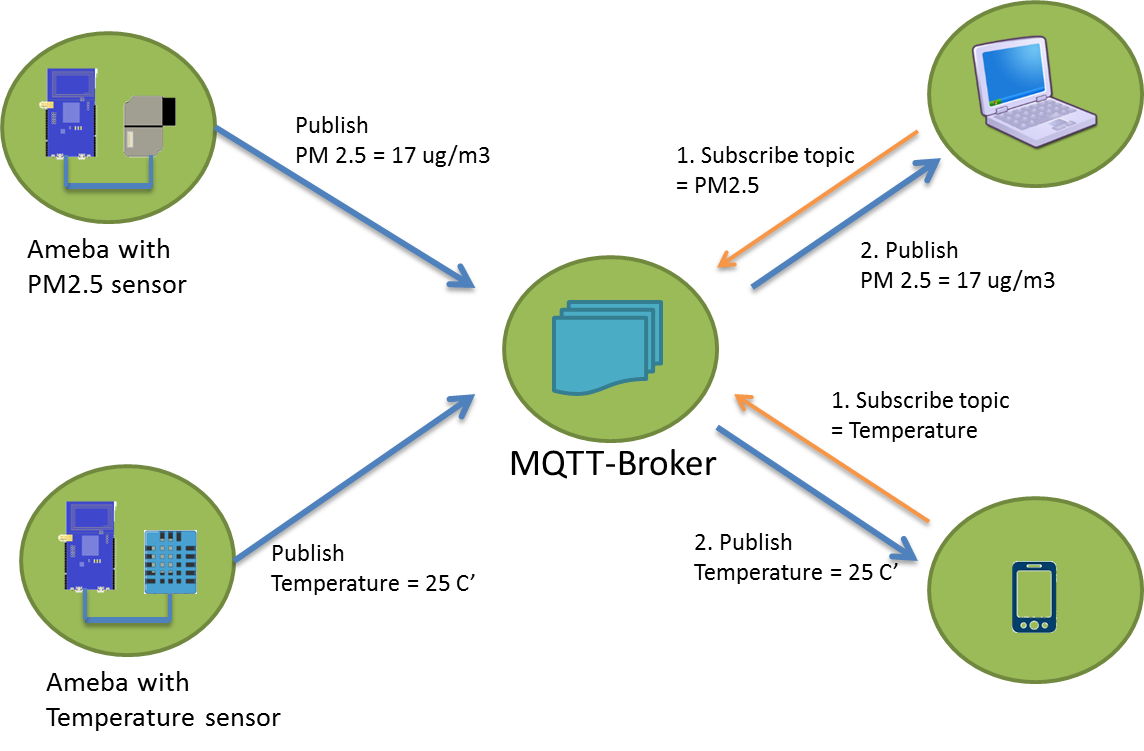
\includegraphics[height=7cm,width=11cm]{hinh/mqtt.png}
	\caption{Một ví dụ mô tả các thiết bị liên lạc với nhau thông qua MQTT broker\cite{mqtt}.}
	\label{fig:mqtt}
\end{figure}


\newpage
\section{THIẾT KẾ HỆ THỐNG}
\subsection{Kiến trúc mô hình hệ thống}
\noindent Kiến trúc hệ thống bao gồm các thành phần: web server, web app, database và hệ thống board điều khiển. 

\begin{figure}[H]
	\centering
	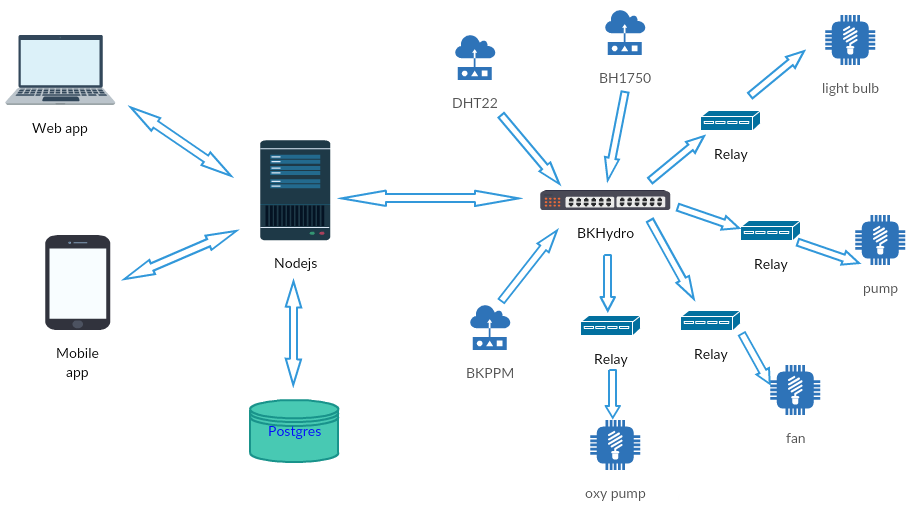
\includegraphics[height=9cm,width=13cm]{hinh/system.png}
	\caption{Kiến trúc hệ thống.}
	\label{fig:system}
\end{figure}


\subsection{Hệ thống board điều khiển}

\subsubsection{Tổng quan mô hình board điều khiển}

\noindent \textbf{Hệ thống board điều khiển chia ra làm 3 thành phần chức năng chính:}
\begin{itemize}
\item Thu thập dữ liệu các cảm biến.
\item Định thời, điều khiển các actuator (máy bơm, sục oxi, đèn chiếu sáng...) theo thời gian thực.
\item Truyền nhận dữ liệu với web-server thông qua môi trường wifi.

\end{itemize}

\noindent \textbf{Các module, cảm biến của hệ thống:}
\begin{itemize}

\item Cảm biến nhiệt độ, độ ẩm: nhiệt đô, độ ẩm được đo bởi module DHT22.

\begin{figure}[H]
	\centering
	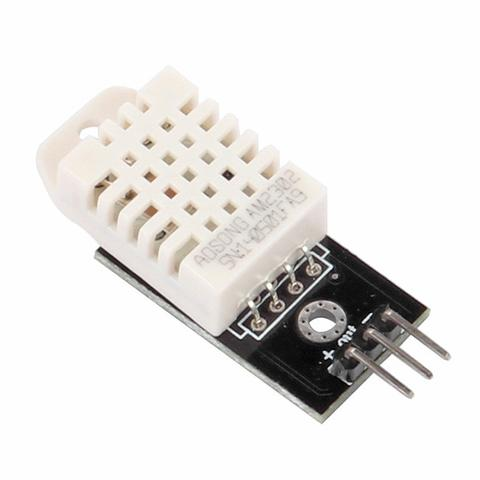
\includegraphics[scale=.3]{hinh/DHT22.jpg}
	\caption{Cảm biến nhiệt độ, độ ẩm\cite{dht22}.}
	\label{fig:DHT22}
\end{figure}


\noindent Thông tin kỹ thuật\cite{dht22}:
\begin{itemize}
\item Nguồn 3-5 VDC.
\item Dòng sử dụng: max là 2.5mA.
\item Đo tốt ở độ ẩm 0x100\%RH, sai số 2-5\%.
\item Đo tốt ở nhiệt độ 0-50\textsuperscript{o}C, sai số 2\textsuperscript{o}C.
\item Tần số lấy mẫu tối đa 0.5Hz (2 giây 1 lần).
\item Kích thước 27mm x 58mm x 13.5mm
\item 3 chân, khoảng cách 0.1 inch.
\end{itemize}

\item Cảm biến đo cường độ ánh sáng: được đo bởi module BH1750.
\begin{figure}[H]
	\centering
	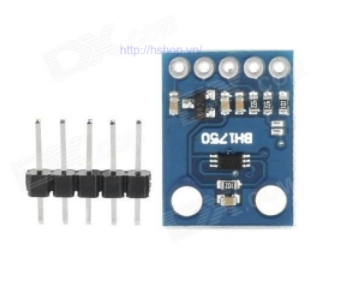
\includegraphics[scale=.8]{hinh/BH175.png}
	\caption{Module BH1750\cite{bh1750}.}
	\label{fig:BH175}
\end{figure}

\noindent Thông tin kỹ thuật\cite{bh1750}:
\begin{itemize}
\item Nguồn: 3-5 VDC.
\item Protocol giao tiếp: I2C
\item Khoảng đo: 1->65535 lux.
\item Đo tốt ở nhiệt độ 0-50\textsuperscript{o}C, sai số 2\textsuperscript{o}C.
\item Kích cỡ: 21x16x3.3 mm.
\end{itemize}

\item Thời gian thực: thời gian thực được đo sử dụng module Realtime clock DS1307. Module có chức năng lưu trữ thông tin ngày tháng năm cũng như giờ phút giây, nó sẽ hoạt đông như một chiếc đồng hồ và có thể xuất dữ liệu ra ngoài qua giao thức I2C. Module được thiết kế kèm theo một viên pin có khả năng cung cấp năng lượng tới 10 năm. Module đi kèm với EEPROM AT14C32 có khả năng lưu trữ lên đến 32Kbit.\\

\begin{figure}[H]
	\centering
	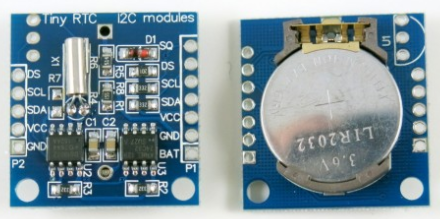
\includegraphics[scale=.4]{hinh/DS1307.PNG}
	\caption{Module Realtime Clock DS1307\cite{ds1307}.}
	\label{fig:DS1307}
\end{figure}


Thông tin kĩ thuật\cite{ds1307}:
\begin{itemize}
\item Nguồn cấp: 5VDC.
\item Khả năng lưu trữ: 32K (EEPROM AT24C32).
\item Protocol: I2C.
\item Có pin chạy độc lập.
\item Tần số ra: 1 HZ.
\item Kích thước: 16x22x23mm.
\end{itemize}

\item Relay: các actuators (Máy bơm nước, sục Oxi, led...) được kích thông qua relay.
\begin{figure}[H]
	\centering
	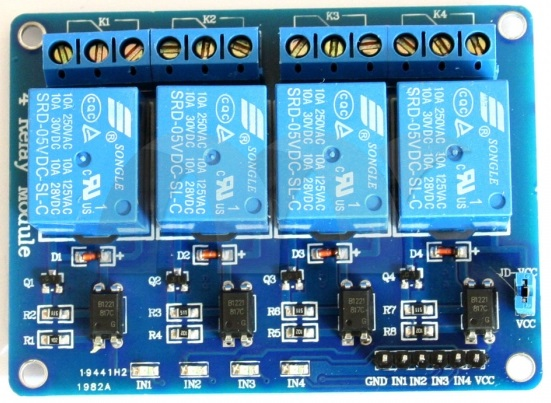
\includegraphics[height=6cm,width=8cm]{hinh/Relay.jpg}
	\caption{Relay\cite{dientuachau}.}
	\label{fig:Relay}
\end{figure}

\noindent Thông số kĩ thuật\cite{dientuachau}:
\begin{itemize}
	\item Nguồn: 5 VDC.
	\item Điện áp kích: 5 VDC.
\end{itemize}

\item Thanh ghi dịch: sử dụng chip 74HC595.
\begin{figure}[H]
	\centering
	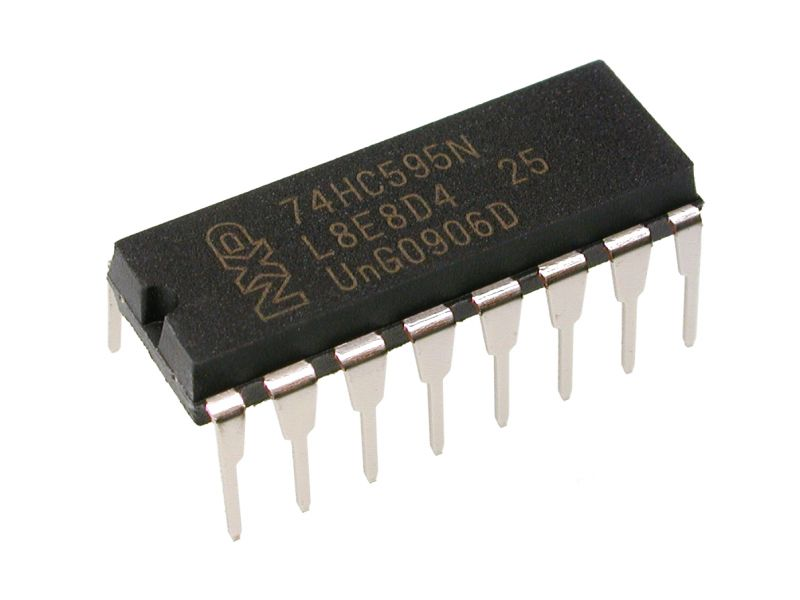
\includegraphics[height=6cm,width=8cm]{hinh/Register.jpg}
	\caption{Thanh ghi dịch\cite{dientuachau}.}
\end{figure}

\noindent Thông số kĩ thuật\cite{dientuachau}:
\begin{itemize}
	\item Nguồn: 5 VDC.
	\item Các chân Output: 5 VDC.
	\item Protocol giao tiếp: SPI.
\end{itemize}


\item Board ARM STM32F03C8T6: được sử dụng để làm board điều khiển các actuators.

\begin{figure}[H]
	\centering
	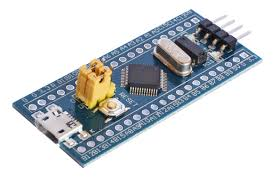
\includegraphics[height=6cm,width=8cm]{hinh/stm32.jpg}
	\caption{Board ARM STM32F03C8T6\cite{dientuachau}.}
\end{figure}

\noindent Thông số kĩ thuật\cite{dientuachau}:
\begin{itemize}
\item RAM: 20KB.
\item Flash: 64KB/128KB.
\end{itemize}

\item Board NodeMCU ESP8266: được sử dụng để làm board truyền nhận dữ liệu qua wifi.
\begin{figure}[H]
	\centering
	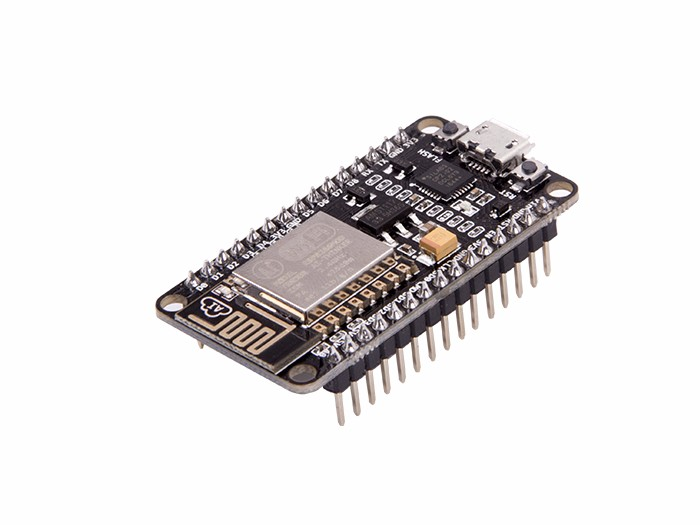
\includegraphics[scale=.4]{hinh/NodeMCU.jpg}
	\caption{Board NodeMCU ESP8266\cite{dientuachau}.}
\end{figure}
\noindent Thông số kĩ thuật\cite{dientuachau}:
	\begin{itemize}
	\item IC chính: ESP8266 Wifi SoC.
	\item Phiên bản firmware: NodeMCU Lua.
	\item Chip nạp và giao tiếp UART: CP2102.
	\item GPIO tương thích hoàn toàn với firmware NodeMCU.
	\item Cấp nguồn: 5VDC MicroUSB hoặc Vin.
	\item GPIO giao tiếp mức 3.3VDC.
	\item Tích hợp LED báo trạng thái, nút Reset, Flash.
	\item Tương thích hoàn toàn với trình biên dịch Arduino.
	\item Kích thước: 25 x 50 mm.
	\end{itemize}

\end{itemize}

\subsubsection{Hoạt động, chức năng}
\noindent \textbf{Sơ đồ hoạt động:}\\

\begin{figure}[H]
	\centering
	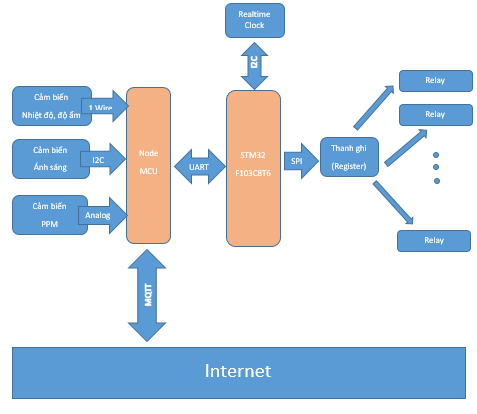
\includegraphics[scale=1]{hinh/mohinh.png}
	\caption{Mô hình tổng quan.}
\end{figure}


\noindent \textbf{Thu thập dữ liệu cảm biến:}\\
\noindent Các cảm biến được kết nối trực tiếp với board NodeMCU và lấy dữ liệu trực tiếp.
\begin{itemize}
	\item Nhiệt độ, độ ẩm: module DHT22 giao tiếp 1 wire với board NodeMCU. Dữ liệu nhiệt độ (C), độ ẩm (\%) được đọc sau mỗi (1s).
	\item Cường độ ánh sáng: module BH1750 giao tiếp I2C với board NodeMCU. Dữ liệu cường độ ánh sáng (lux) được đọc sau mỗi (1s).
	\item Module ppm hoạt động độc lập, đọc dữ liệu từ môi trường dung dịch, xuất đầu ra analog được đọc bởi board NodeMCU sau mỗi (1s).
	\item Định thời đọc dữ liệu cảm biến sử dụng timer, timeout là 1s.
\end{itemize}

\noindent Hoạt động đọc, quản lí dữ liệu cảm biến sẽ được thực hiện bởi 1 đối tượng:
\begin{itemize}
\item Quản lí các thông tin: nhiệt độ, độ ẩm, PPM, ánh sáng.
\item Hoạt động độc lập, định thời đọc dữ liệu theo sơ đồ Hình 26.

\begin{figure}[H]
	\centering
	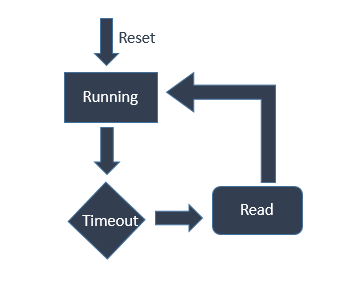
\includegraphics[scale=0.9]{hinh/sensor.PNG}
	\caption{Hoạt động độc lập, định thời đọc dữ liệu.}
\end{figure}

\end{itemize}

\noindent \textbf{Điều khiển các actuators}

\textbf{Thông số các actuator:}

\begin{itemize}

\item Máy bơm nước:

\begin{figure}[H]
	\centering
	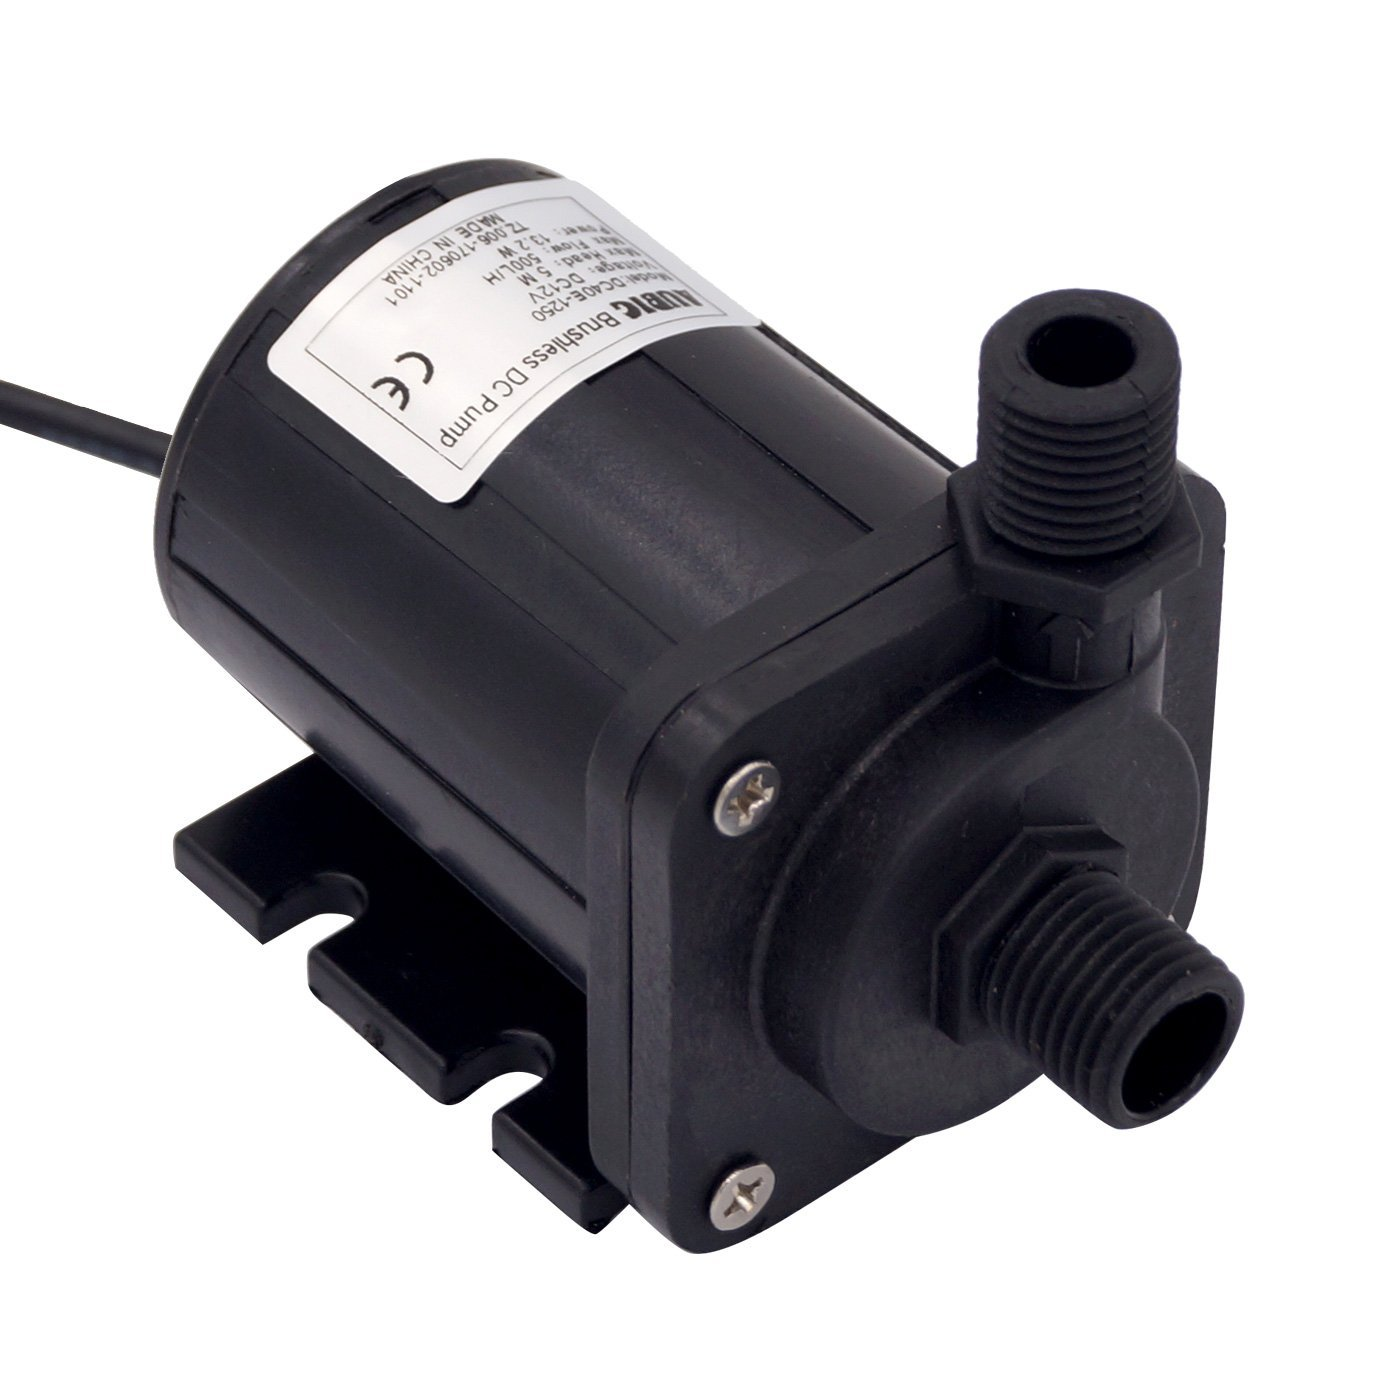
\includegraphics[scale=0.2]{hinh/pump.jpg}
	\caption{Máy bơm nước.}
\end{figure}

\begin{itemize}
\item Nguồn: 12 VDC.
\item Công suất: 500L/h
\item Khả năng phun nước độ cao 2m phương thẳng đứng.
\end{itemize}


\item  Máy sục oxy:

\begin{figure}[H]
\centering
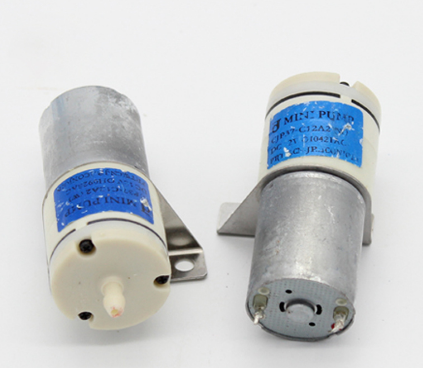
\includegraphics[scale=0.75]{hinh/oxi.png}
\caption{Máy sục oxy.}
\end{figure}

\begin{itemize}
\item Nguồn: 12 VDC.
\end{itemize}


\item Đèn chiếu sáng:
\begin{figure}[H]
	\centering
	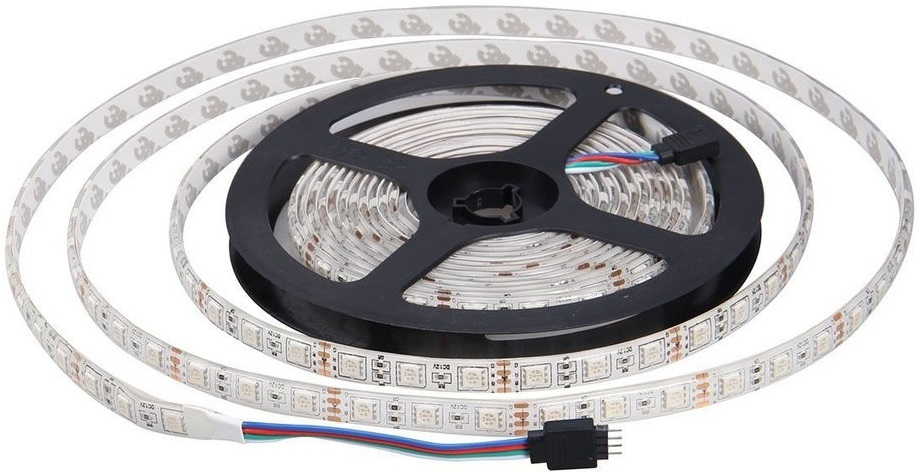
\includegraphics[scale=0.4]{hinh/led.jpg}
	\caption{Đèn led.}
\end{figure}
\begin{itemize}
\item Nguồn: 12 VDC. 
\item Công suất: 15W/m
\end{itemize}

\end{itemize}

\newpage
\textbf{Cách điều khiển các actuator:}
\begin{itemize}

\item Hoạt động của thanh ghi dịch:

\begin{figure}[H]
	\centering
	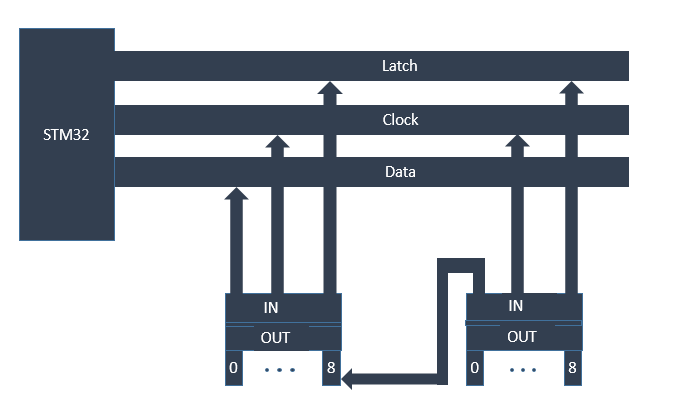
\includegraphics[scale=0.8]{hinh/stm_register.PNG}
	\caption{Hoạt động của thanh ghi dịch.}
\end{figure}

\noindent Giao tiếp của thanh ghi dịch với board điều khiển là SPI, các chân điều khiển:
\begin{itemize}
\item DATA: chân dữ liệu.
\item LATCH: đẩy dữ liệu từ thanh ghi bên trong chip xuống các pinout, cụ thể là 8 chân, điện áp ra là 5V.
\item CLOCK: tín hiệu clock lấy từ board điều khiển.
\end{itemize}

\noindent Chân DATA của thanh ghi đầu tiên sẽ nối với chân tín hiệu đầu ra của board điều khiển, DATA của các thanh ghi tiếp theo sẽ lấy từ pinout thứ 9 của thanh ghi liền trước nó.

\item Các actuators sẽ được kích hoạt trực tiếp thông qua relay:

\begin{figure}[H]
	\centering
	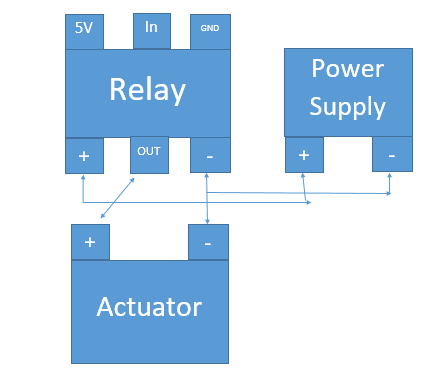
\includegraphics[scale=0.8]{hinh/actuator.PNG}
	\caption{Hoạt động của các actuators.}
\end{figure}

\item Tín hiệu điều khiển relay sẽ lấy từ thanh ghi: \\

\begin{figure}[H]
	\centering
	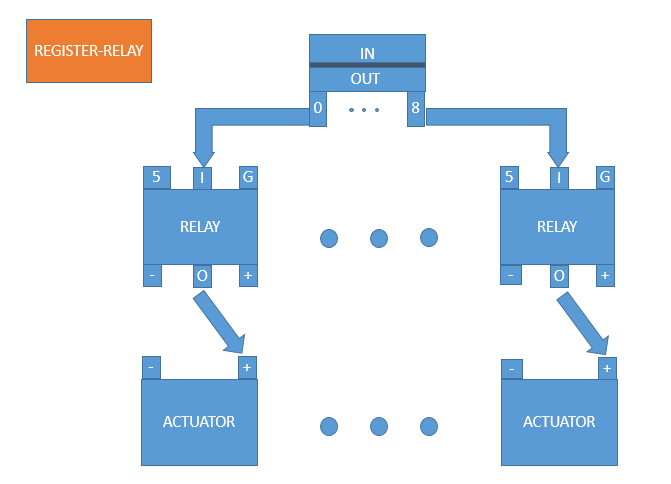
\includegraphics[scale=0.7]{hinh/register_relay.PNG}
	\caption{Hoạt động của tín hiệu điều khiển relay.}
\end{figure}

\end{itemize}
\newpage
\noindent \textbf{Thời gian thực:}

\begin{itemize}
\item Module Realtime Clock DS1307 sẽ hoạt động độc lập với pin, cụ thể, các thông số thời gian thực trong module không bị ảnh hưởng bởi nguồn nuôi của toàn mạch.
\item Thời gian thực (year, month, day, hour, min, sec) có thể được đọc và ghi bởi board điều khiển, cụ thể là NodeMCU.

\begin{figure}[H]
	\centering
	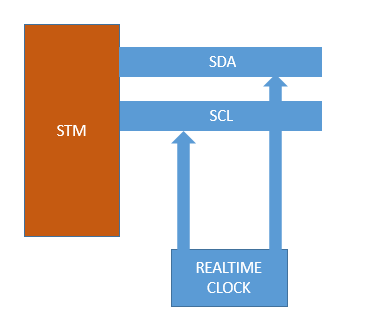
\includegraphics[scale=0.8]{hinh/Node_Realtime.PNG}
	\caption{Hoạt động Thời gian thực.}
\end{figure}

\item Định thời đọc dữ liệu thời gian thực sử dụng timer, timeout là 1/3s.

\end{itemize}

\noindent \textbf{Tổ chức, quản lí hoạt động của các actuators.}

\begin{itemize}
\item Chân điều khiển: Các actuator được điểu khiển (tắt, mở) thông qua tín hiệu các chân của thanh ghi dịch (74HC595) và relay nên không phụ thuộc vào các pinout của board điều khiển (STM32F103C8T6). Có thể tăng số chân điều khiển (cũng như tăng số actuators) bằng cách thêm các thanh ghi dịch, số pinout sử dụng luôn là 3, cụ thể là các chân SPI (DATA, LATCH, CLOCK).

\item Thời gian biểu:\\
Mỗi actuator sẽ hoạt động theo một thời gian biểu, cụ thể trong thủy canh:

\begin{center}
\begin{tabularx}{\linewidth}{ |X|X|X|X| }
\hline
Start & Duration & Repeat Interval & Stop\\
\hline
Thời điểm bắt đầu hoạt động. & Thời lượng actuator được mở. & Thời lượng tắt actuator giữa hai lần mở. & Thời điểm tắt actuator cho đến thời điểm Start kế tiếp.\\
\hline
\end{tabularx}
\end{center}

\noindent Định dạng thời gian cho mỗi kiểu như trên là hhmmss. Mỗi thời gian biểu cho mỗi ngày sẽ bao gồm nhiều mẫu như trên, ví dụ với máy bơm: Máy bơm sẽ bắt đầu bơm nước từ 08:00:00 (start), mỗi lần tưới sẽ kéo dài trong 15s (duration), sau đó sẽ tắt trong 10s (repeat interval), lại bật tiếp 15s, cứ thế cho đến 09:00:00 (stop).


\item Lifetime của mỗi actuator (phần mềm).

\begin{figure}[H]
	\centering
	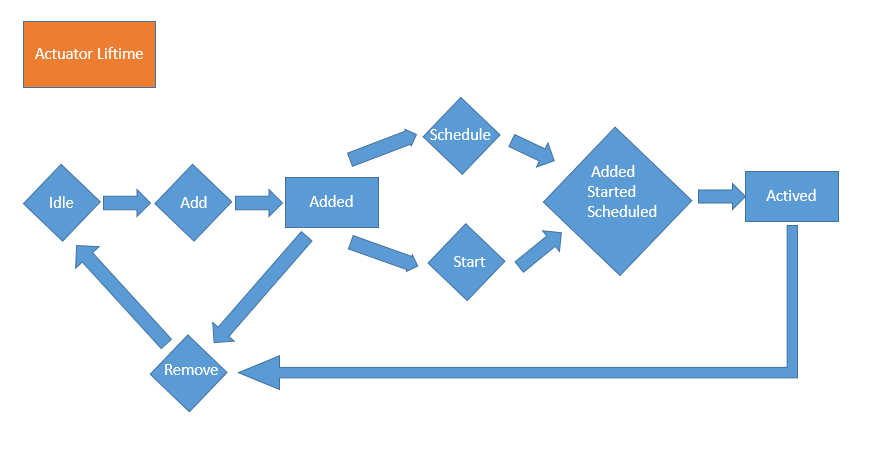
\includegraphics[scale=0.7]{hinh/actuator_lifetime.PNG}
	\caption{Actuator lifetime.}
\end{figure}

\noindent Mỗi actuator sẽ là một đối tượng (phần mềm), giải thích lifetime:
	\begin{itemize}
	\item Ban đầu, sẽ không có actuator nào, các actuator không được sét tĩnh.
	\item  Khi nhận gói tin (Add) từ web-server, một đối tượng actuator sẽ được tạo ra, là một node trong danh sách liên kết (linked-list) các actuators. Mỗi đối tượng chứa các thông tin:
\begin{itemize}
\item Actuator ID: định danh của actuator.
\item Primary: là actuator chính hay phụ.
\item Schedule: thời gian biểu hoạt động.
\item Started: điều kiện để hoạt động.
\end{itemize}

	\item Sau khi được add (Added), đối tượng sẽ chờ nhận thêm hai gói tin (thứ tự bất kì) là (Start) và (Schedule) để chuyển sang trạng thái (Actived).
		\begin{itemize}
			\item Nhận gói (Schedule): đối tượng sẽ lưu lại thông tin schedule.
			\item Nhận gói (Start): đối tượng sẽ cập nhập thông tin (Started). 
		\end{itemize}			

	\item Ở trạng thái (Added) và (Actived) khi nhận được gói (Remove) , đối tượng sẽ bị xóa.
	\item Ở trạng thái (Actived), đối tượng actuator sẽ hoạt động với thông tin (Schedule) theo thời gian thực đọc được từ module Realtime Clock DS1307.
	\end{itemize}
\item Lưu trữ thông tin actuator.

	\begin{itemize}
	\item Để đáp ứng tính độc lập của board điều khiển, các thông tin của mỗi actuator sẽ được lưu lại trong bộ nhớ ROM, tránh trường hợp reset của board ( có thể do nhiều nguyên nhân khác nhau: mất điện, crash..).
	\item Thông tin actuator được thêm trong trong lúc board đang hoạt động ở thời điểm ngẫu nhiên (runtime), không sét tĩnh, đây là ưu điểm của giải pháp này, cho phép mở rộng, thay đổi các actuator.
	\item Bộ nhớ lưu trữ là EEPROM, phân vùng lưu trữ sẽ nêu cụ thể trong phần (Lưu trữ dữ liệu) nằm trên board NodeMCU.
	\item Cấu trúc dữ liệu lưu trữ được nêu cụ thể trong phần hiện thực.
	\item Dưới đây là cách hoạt động của việc lưu trữ (Save) và tải lại (Load). Qui ước: Các sự kiện (Add), (Start), (Schedule), (Update), (Remove) sẽ được gọi chung là (Update). Các trạng thái (Added), (Actived) được gọi chung là (Running).\\\\
	
	\end{itemize}
	
\begin{figure}[H]
	\centering
	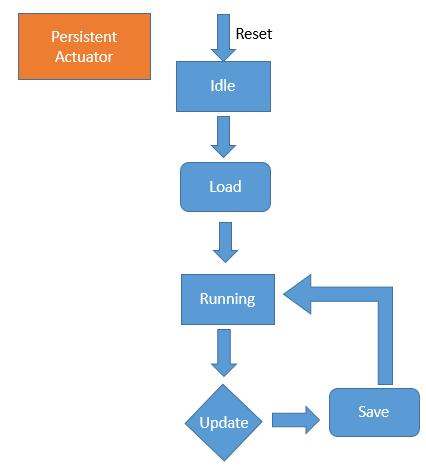
\includegraphics[scale=.6]{hinh/persistent_actuator.PNG}
	\caption{Hoạt động lưu trữ thông tin actuator.}
\end{figure}


\end{itemize}

\noindent \textbf{Truyền nhận dữ liệu với giao thức MQTT}
	\begin{itemize}
	\item Đối tượng thực hiện công việc này hoạt động trên board NodeMCU với vai trò là một MQTT Client, bao gồm:
		\begin{itemize}
		\item Lưu trữ các thông tin:
			\begin{itemize}
			\item	MQTT broker.
			\item	MQTT port.
			\item	MQTT subcribe channel.
			\item	MQTT publish channel.
			\end{itemize}
		\item	Các chức năng:
			\begin{itemize}
				\item Publish: truyền dữ liệu tới kênh web-server đăng kí( cũng đóng vai trò là một MQTT Client).
				\item	Subcribe: đăng kí kênh nhận dữ liệu từ web-server.
			\end{itemize}

		\end{itemize}
		\item Các thông tin của đối tượng MQTT Client cũng được lưu trữ trong ROM, nêu trong phần (lưu trữ dữ liệu), và cho phép cấu hình (cấu hình WiFi).
		\item Đối tượng hoạt động độc lập theo sơ đồ dưới:
		
			\begin{figure}[H]
				\centering
				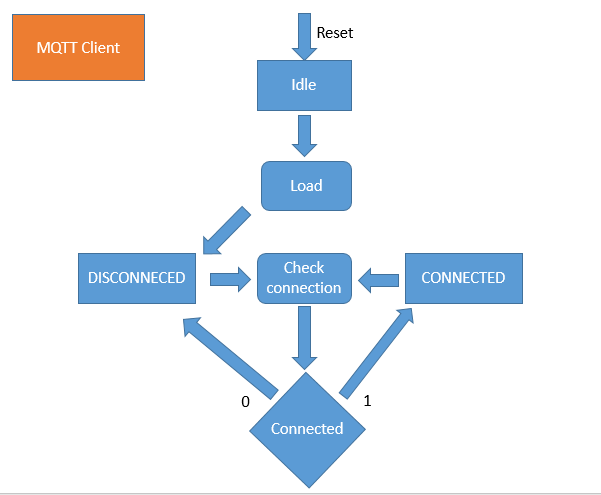
\includegraphics[scale=.6]{hinh/mqtt_client.PNG}		
				\caption{MQTT client.}
			\end{figure}
			
	\end{itemize}
\noindent	\textbf{Cấu hình, hoạt động của các chế độ WiFi}

	\begin{itemize}
	\item	Board NodeMCU cho phép hoạt động ở 3 chế độ:
		\begin{itemize}
		\item	Station: đóng vai trò là một thiết bị kết nối vào mạng wifi tương tự như điện thoại.
		\item	Access Point: Phát wifi, cho phép thiết bị khác kết nối vào.
		\item	Both: cả hai chức năng trên.
		\end{itemize}

	\item	Ở dự án này, 2 chế độ được sử dụng là (Station) và (Access Point), cụ thể:
		\begin{itemize}
		\item	Station: Ở chế độ này, board sẽ thực hiện chức năng của MQTT Client.
		\item	Access Point: cung cấp chức năng của một Web-server nhỏ, cho phép cấu hình:
			\begin{itemize}
				\item	Các thông  số wifi (tên wifi, mật khẩu) khi board hoạt động ở (Station). 
				\item	Thông tin của đối tượng MQTT Client (broker, port...).
				\item	Các thông tin sau khi cấu hình sẽ được lưu trữ trong EEPROM.
			\end{itemize}
		\end{itemize}


	\item	Chức năng chuyển chế độ sẽ được thực hiện bởi một nút nhấn.
	\item	Các chế độ hoạt động như sau:\\

	\end{itemize}
		
			\begin{figure}[H]
				\centering
				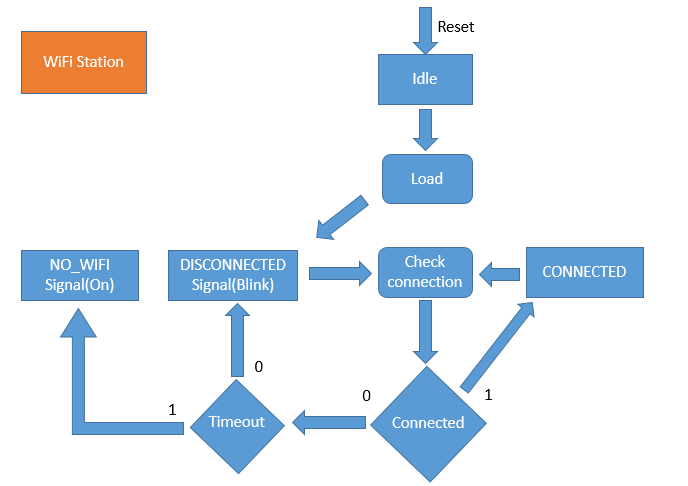
\includegraphics[scale=.6]{hinh/wifi_station.PNG}
				\caption{Wifi station.}
			\end{figure}
		
			\begin{figure}[H]
				\centering
				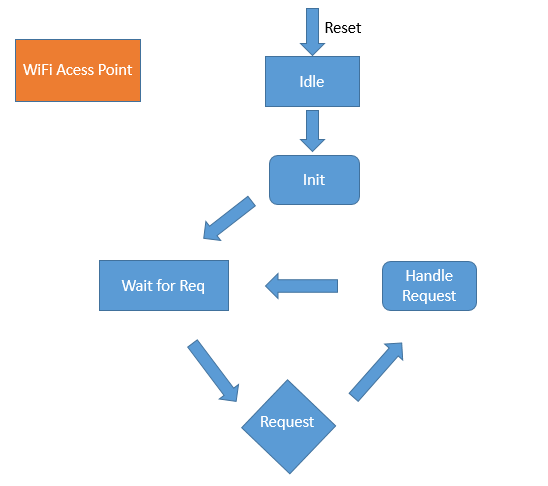
\includegraphics[scale=.6]{hinh/wifi_ap.PNG}			
				\caption{Wifi AP.}
			\end{figure}
			
			\begin{figure}[H]
				\centering
				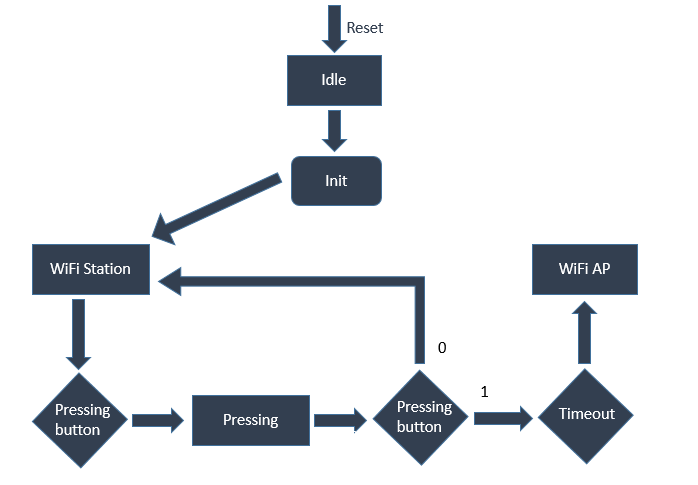
\includegraphics[scale=.6]{hinh/wifi_application.PNG}
				\caption{Wifi application.}
			\end{figure}

\noindent	\textbf{Đệm dữ liệu (FIFO)}
	\begin{itemize}
	\item Chức năng:
		\begin{itemize}
		\item	Để đảm bảo tính ổn định, đồng bộ giữa quá trình nhận - xử lí các gói tin.
		\item	Giảm tải thời gian xử lí interrupt (có khả năng gây xung đột các task).
		\end{itemize}
	\item	Các vị trí cần sử dụng bộ đệm:
		\begin{itemize}
		\item	Khi  nhận các gói tin serial (uart).
		\item	Khi gửi các gói tin MQTT: việc gửi các gói tin MQTT là thông qua môi trường wifi, nên không phải lúc nào cũng đảm bảo tính kết nối giữa client với broker, vì vậy cần bộ đệm để lưu trữ các gói tin trước khi gửi.
		\end{itemize}
	\item	Cấu trúc bộ đệm: các gói tin xếp theo thứ tự FIFO.
	\end{itemize}


\noindent	\textbf{Lưu trữ dữ liệu}
	\begin{itemize}
	\item	Các thông tin cần được lưu trữ trong EEPROM:
		\begin{itemize}
		\item	Thông tin wifi station: ssid, password.
		\item	Thông tin MQTT: broker, port, subcribe channel, publish channel.
		\item	Actuators.
		\end{itemize}
	\item	Việc lưu trữ và quản lí sẽ do một đối tượng thực hiện.
	
	\item	EEPROM đặt trên board NodeMCU, đối tượng Actuators lại hoạt động trên board STM nên sẽ cần một giao thức để tải dữ liệu từ NodeMCU sang STM. 

	\end{itemize}

\noindent	\textbf{Giao tiếp giữa NodeMCU và STM32F103C8T6}
	\begin{itemize}
	\item Các gói tin trao đổi giữa STM và Node MCU:
		\begin{table}[H]
		\centering
		\begin{tabular}{|l|l|}
		\hline
		Packet & Send\\
		\hline
		Web-server packets (1) & NodeMCU\\
		\hline
		Actuators Info (2) & STM, NodeMCU\\
		\hline
		Load actuators request (3) & STM\\
		\hline
		Load done (4) & Node MCU\\
		\hline
		Setting (5) & STM\\
		\hline
		\end{tabular}
		\caption{Các gói tin trao đổi giữa STM và Node MCU.}
		\end{table}
		
		\begin{itemize}
			\item (1) Các gói tin NodeMCU nhận được từ web - server sẽ được chuyển cho STM.
			\item (2) Dữ liệu trạng thái các actuators: 
			\begin{itemize}
				\item STM gửi NodeMCU: Actuator nào thay đổi trạng thái (update) sẽ được gửi từ STM để cập nhật trạng thái tại bộ nhớ EEPROM trên NodeMCU.
				\item NodeMCU gửi STM: khi nhận được yêu cầu tải lại (load) từ STM, NodeMCU sẽ tải lại dữ liệu trên EEPROM và gửi cho STM.
			\end{itemize}
			
			\item (3) Mỗi khi reset, board STM sẽ tải lại dữ liệu trạng thái các actuator bằng cách gửi gói tin này.
			\item (4) NodeMCU thông báo đã tải hết dữ liệu các actuators.
			\item (5) STM thông báo nếu đang trong thời gian hoạt động mùa vụ cho NodeMCU, khi nằm ngoài thời gian hoạt động, NodeMCU sẽ không gửi dữ liệu các cảm biến cho web - server.
		\end{itemize}
	
	\item Giao thức lớp dưới được sử dụng là UART.
	\item Một giao thức đơn giản được xây dựng trên lớp UART nhằm:
		\begin{itemize}
		\item	Truyền, nhận các gói tin lớn.
		\item	Đảm bảo tính toàn vẹn của gói tin.
		\item Cấu trúc giao thức:
			
			\begin{figure}[H]
				\centering
				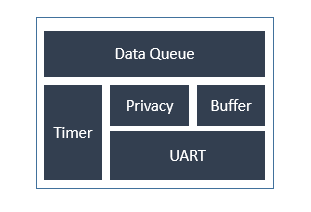
\includegraphics[scale=1]{hinh/uart_protocol.PNG}
				\caption{Cấu trúc giao thức UART.}
			\end{figure}
			
		  \begin{itemize}
		  \item	Các thành phần chính:
		  	\begin{itemize}
		  		\item	Timer: định thời đọc dữ liệu có sẵn trong UART ở lớp dưới.
				\item	Buffer: bộ đệm tạm thời cho dữ liệu rời rạc.
				\item	Privacy: chính sách truyền nhận.
				\item	Data Queue: gói tin toàn vẹn được đưa vào queue (FIFO), nêu cụ thể trong phần (Đệm dữ liệu). 
				\item	UART: giao thức truyền nhận lớp dưới.
		  	\end{itemize}
		  	
		  	
			\begin{figure}[H]
				\centering
				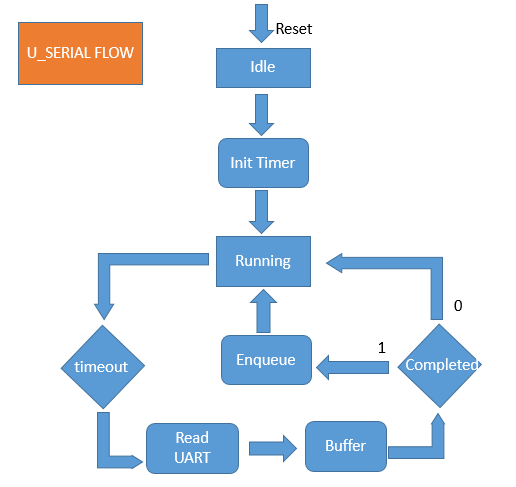
\includegraphics[scale=.6]{hinh/uart_flow.PNG}
				\caption{Cách hoạt động của giao thức UART.}
			\end{figure}	  	
		  	
		  \end{itemize}
		\end{itemize}
	\end{itemize}

\subsubsection{Kiến trúc phần mềm}

\begin{itemize}

\item Sequence diagram

\begin{figure}[H]
	\centering
	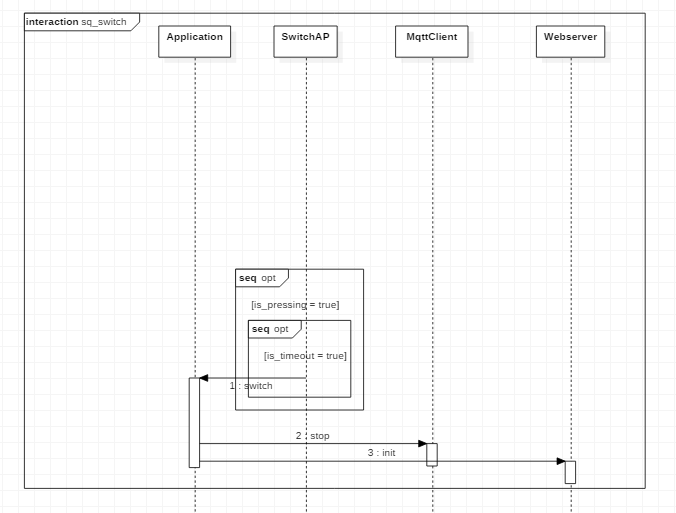
\includegraphics[scale=.9]{hinh/sq_switch_wifi.PNG}
	\caption{Cấu hình wifi.}
\end{figure}

\begin{figure}[H]
	\centering
	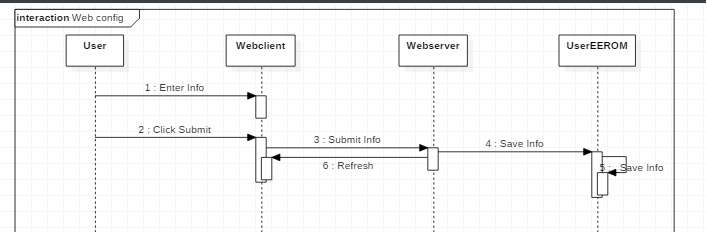
\includegraphics[scale=.8]{hinh/sq_web.PNG}
	\caption{Hoạt động của web-server hoạt động trên board Node MCU.}
\end{figure}

\begin{figure}[H]
	\centering
	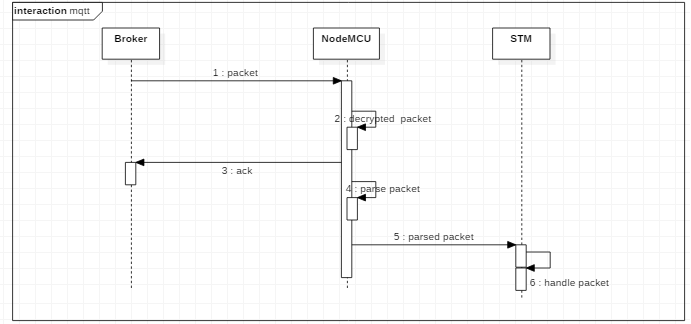
\includegraphics[scale=.8]{hinh/sq_mqtt.PNG}
	\caption{Truyền nhận dữ liệu.}
\end{figure}

\newpage
\item Class diagram

\begin{itemize}
	\item Các class hoạt động trên board NodeMCU:
	
	\begin{figure}[H]
		\centering
		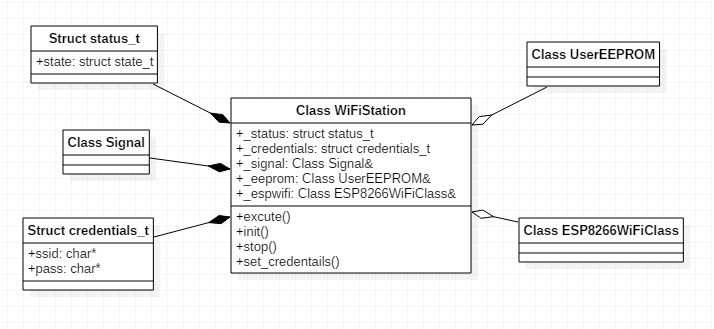
\includegraphics[scale=.85]{hinh/class_wifistation.PNG}
		\caption{WifiStation.}
	\end{figure}

\begin{figure}[H]
\centering
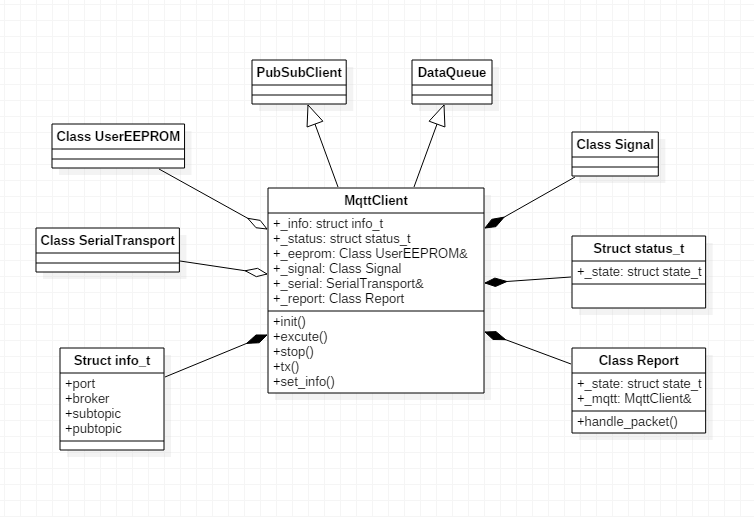
\includegraphics[scale=.85]{hinh/class_mqttclient.PNG}
\caption{MqttClient.}
\end{figure}

\begin{figure}[H]
\centering
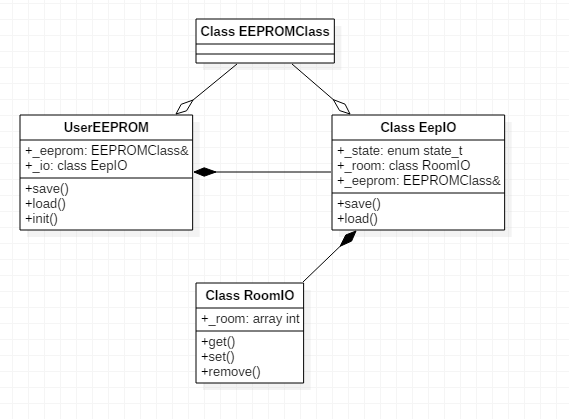
\includegraphics[scale=.85]{hinh/class_usereeprom.PNG}
\caption{UserEEPROM.}
\end{figure}

\begin{figure}[H]
\centering
\includegraphics[scale=.85]{hinh/class_sensor.PNG}
\caption{Sensor.}
\end{figure}

\begin{figure}[H]
\centering
\includegraphics[scale=.65]{hinh/class_serialtransport.PNG}
\caption{SerialTransport.}
\end{figure}

\begin{figure}[H]
\centering
\includegraphics[scale=.85]{hinh/class_webserver.PNG}
\caption{ Webserver.}
\end{figure}

\begin{figure}[H]
\centering
\includegraphics[scale=.9]{hinh/class_switchap.PNG}
\caption{SwitchAP.}
\end{figure}

\begin{figure}[H]
\centering
\includegraphics[scale=.9]{hinh/class_nodeapplication.PNG}
\caption{ Application.}
\end{figure}

\newpage
	\item Các class hoạt động trên board STM:

\begin{figure}[H]
\centering
\includegraphics[scale=.85]{hinh/class_serialtransport.PNG}
\caption{SerialTransport.}
\end{figure}

\begin{figure}[H]
\centering
\includegraphics[scale=.85]{hinh/class_stmapplication.PNG}
\caption{Apllication.}
\end{figure}

\begin{figure}[H]
\centering
\includegraphics[scale=.75]{hinh/class_actuator.PNG}
\caption{Actuator.}
\end{figure}

\end{itemize}

\end{itemize}
\newpage
\subsection{Ứng dụng web}
\subsubsection{Sơ đồ use case}
\indent \textbf{Các chức năng của tài khoản khi chưa thực hiện đăng nhập tài khoản.}\\

\begin{figure}[H]
\centering
\includegraphics[scale=.9]{hinh/uc_web1.png}
\caption{Các chức năng của khách.}
\end{figure}

\newpage
\begin{figure}[H]
\centering
\includegraphics[scale=.9]{hinh/reg.png}
\caption{Đăng ký.}
\end{figure}

\begin{table}[!htp]
\centering
\begin{tabularx}{\linewidth}{ |c||c|c|c| }
\hline
ID & Name & Created by & Created at\\
UC\_REG\_001 & Đăng ký tài khoản & Tạ Chí Tây & 20/3/2017\\
\hline
\multicolumn{4}{|X|}{\textbf{Actor:} Khách }\\
\hline
\multicolumn{4}{|X|}{\textbf{Mô tả ngắn gọn:} khách có thể đăng ký thành viên }\\
\hline
\multicolumn{4}{|X|}{\textbf{Kịch bản chính:}}\\
\multicolumn{4}{|X|}{1. Người dùng khởi động khung đăng ký bằng cách nhấn nút Register}\\
\multicolumn{4}{|X|}{
2.	Người dùng nhập các thông tin cần thiết trong khung đăng ký và nhấn Register.}\\
\multicolumn{4}{|X|}{
3.	Hệ thống tạo người dùng mới}\\
\multicolumn{4}{|X|}{
4.	Hệ thống thông báo người dùng đã đăng ký thành công.}\\
\hline
\multicolumn{4}{|X|}{\textbf{Kịch bản phụ:}}\\
\multicolumn{4}{|X|}{2.1. Các ô thông tin bị để trống hoặc nhập sai định dạng, mật khẩu không khớp, email đã đăng ký thì hệ thống sẽ thông báo.}\\
\hline
\multicolumn{4}{|X|}{\textbf{Các quan hệ khác:}}\\
\multicolumn{4}{|X|}{- Include: nhập họ tên}\\
\multicolumn{4}{|X|}{- Include: nhập email}\\
\multicolumn{4}{|X|}{- Include: nhập mật khẩu}\\
\multicolumn{4}{|X|}{- Include: nhập số điện thoại}\\
\hline
\end{tabularx}
\caption{Mô tả use case đăng ký.}
\end{table}

\begin{figure}[H]	
	\centering
	\includegraphics[scale=.9]{hinh/login.png}
	\caption{Đăng nhập.}
\end{figure}

\begin{table}[!htp]
\centering
\begin{tabularx}{\linewidth}{ |c||c|c|c| }
\hline
ID & Name & Created by & Created at\\
UC\_LOGIN\_001 & Đăng nhập & Tạ Chí Tây & 20/3/2017\\
\hline
\multicolumn{4}{|X|}{\textbf{Actor:} Khách }\\
\hline
\multicolumn{4}{|X|}{\textbf{Mô tả ngắn gọn:} khách có thể đăng nhập vào hệ thống }\\
\hline
\multicolumn{4}{|X|}{\textbf{Tiền điều kiện:} người dùng đã đăng ký thành công}\\
\hline
\multicolumn{4}{|X|}{\textbf{Kịch bản chính:}}\\
\multicolumn{4}{|X|}{1. Người dùng khởi động khung đăng nhập bằng cách nhấn vào nút Login.}\\
\multicolumn{4}{|X|}{
2.	Người dùng nhập email và mật khẩu vào các ô tương ứng và nhấn nút Sign In.}\\
\multicolumn{4}{|X|}{
3.	Hệ thống xác thực người dùng thông qua email và mật khẩu.}\\
\multicolumn{4}{|X|}{
4.	Hệ thống thông báo người dùng đã đăng nhập thành công.}\\
\hline
\multicolumn{4}{|X|}{\textbf{Kịch bản phụ:}}\\
\multicolumn{4}{|X|}{2.1 Tên truy cập không tồn tại trong cơ sở dữ liệu hoặc mật khẩu không chính xác. Hệ thống hiển thị lại biểu mẫu Đăng nhập và hiển thị thông báo lỗi trên màn hình và yêu cầu nhập lại.}\\
\multicolumn{4}{|X|}{5. Nhấn vào nút "Quên mật khẩu". Hệ thống sẽ gửi đường link reset mật khẩu đến email của người dùng và thông báo cho người dùng biết.}\\
\hline
\multicolumn{4}{|X|}{\textbf{Các quan hệ khác:}}\\
\multicolumn{4}{|X|}{- Include: nhập email}\\
\multicolumn{4}{|X|}{- Include: nhập mật khẩu}\\
\hline
\end{tabularx}
\caption{Mô tả use case đăng nhập.}
\end{table}

\newpage
\indent \textbf{Các chức năng của tài khoản thành viên sau khi đăng nhập.}\\

\begin{figure}[H]
	\centering
	\includegraphics[scale=.9]{hinh/cntv.png}
	\caption{Các chức năng của thành viên.}
\end{figure}

\newpage
\begin{figure}[H]
	\centering
	\includegraphics[scale=.6]{hinh/tdtt.png}
	\caption{Use case thay đổi thông tin.}
\end{figure}

\begin{table}[!htp]
\centering
\begin{tabularx}{\linewidth}{ |c||c|c|c| }
\hline
ID & Name & Created by & Created at\\
UC\_CHANGEINFO\_001 & Thay đổi thông tin cá nhân & Tạ Chí Tây & 20/3/2017\\
\hline
\multicolumn{4}{|X|}{\textbf{Actor:} Thành viên }\\
\hline
\multicolumn{4}{|X|}{\textbf{Mô tả ngắn gọn:} người dùng nhập tên và số điện thoại mình muốn thay đổi để cập nhật thông tin}\\
\hline
\multicolumn{4}{|X|}{\textbf{Tiền điều kiện:} người dùng đã đăng nhập thành công}\\
\hline
\multicolumn{4}{|X|}{\textbf{Kịch bản chính:}}\\
\multicolumn{4}{|X|}{1. Người dùng khởi động khung thay đổi thông tin bằng cách nhấn vào nút Edit.}\\
\multicolumn{4}{|X|}{
2.	Người dùng nhập tên và số điện thoại mới vào các ô tương ứng và nhấn nút OK.}\\
\multicolumn{4}{|X|}{
3.	Hệ thống xác thực người dùng và cập nhật thông tin.}\\
\multicolumn{4}{|X|}{
4.	Hệ thống thông báo người dùng đã thay đổi thành công.}\\
\hline
\multicolumn{4}{|X|}{\textbf{Kịch bản phụ:}}\\
\multicolumn{4}{|X|}{\makecell[l]{2.1    Người dùng để các ô nhập rỗng, hệ thống sẽ báo lỗi.}}\\
\hline
\multicolumn{4}{|X|}{\textbf{Các quan hệ khác:}}\\
\multicolumn{4}{|X|}{- Include: nhập tên}\\
\multicolumn{4}{|X|}{- Include: nhập số điện thoại}\\
\hline
\end{tabularx}
\caption{Mô tả use case hay đổi thông tin cá nhân.}
\end{table}

\begin{table}[!htp]
\centering
\begin{tabularx}{\linewidth}{ |c||c|c|c| }
\hline
ID & Name & Created by & Created at\\
UC\_CHANGEINFO\_002 & Thay đổi ảnh cá nhân & Tạ Chí Tây & 20/3/2017\\
\hline
\multicolumn{4}{|X|}{\textbf{Actor:} Thành viên }\\
\hline
\multicolumn{4}{|X|}{\textbf{Mô tả ngắn gọn:} người dùng thay đổi ảnh đại diện của mình}\\
\hline
\multicolumn{4}{|X|}{\textbf{Tiền điều kiện:} người dùng đã đăng nhập thành công}\\
\hline
\multicolumn{4}{|X|}{\textbf{Kịch bản chính:}}\\
\multicolumn{4}{|X|}{1. Người dùng khởi động khung thay đổi ảnh cá nhân bằng cách nhấn chọn "Change avatar".}\\
\multicolumn{4}{|X|}{
2.	Người dùng chọn đường dẫn đến tập tin ảnh mới trên máy và nhấn OK.}\\
\multicolumn{4}{|X|}{
3.	Hệ thống xác thực người dùng và cập nhật thông tin.}\\
\multicolumn{4}{|X|}{
4.	Hệ thống thông báo người dùng đã thay đổi thành công.}\\
\hline
\multicolumn{4}{|X|}{\textbf{Kịch bản phụ:}}\\
\multicolumn{4}{|X|}{2.1    Người dùng không chọn đường dẫn thì hệ thống sẽ thông báo lỗi.}\\
\hline
\end{tabularx}\\
\caption{Use case thay đổi hình ảnh cá nhân.}
\end{table}

\begin{table}[!htp]
\centering
\begin{tabularx}{\linewidth}{ |c||c|c|c| }
\hline
ID & Name & Created by & Created at\\
UC\_CHANGEINFO\_003 & Thay đổi mật khẩu & Tạ Chí Tây & 20/3/2017\\
\hline
\multicolumn{4}{|X|}{\textbf{Actor:} Thành viên }\\
\hline
\multicolumn{4}{|X|}{\textbf{Mô tả ngắn gọn:} người dùng thay đổi mật khẩu của mình}\\
\hline
\multicolumn{4}{|X|}{\textbf{Tiền điều kiện:} người dùng đã đăng nhập thành công}\\
\hline
\multicolumn{4}{|X|}{\textbf{Kịch bản chính:}}\\
\multicolumn{4}{|X|}{1. Người dùng khởi động khung thay đổi mật khẩu bằng cách nhấn nút "Change password".}\\
\multicolumn{4}{|X|}{
2.	Người dùng nhập thông tin vào các ô tương ứng và nhấn OK.}\\
\multicolumn{4}{|X|}{
3.	Hệ thống xác thực người dùng và cập nhật thông tin.}\\
\multicolumn{4}{|X|}{
4.	Hệ thống thông báo người dùng đã thay đổi thành công.}\\
\hline
\multicolumn{4}{|X|}{\textbf{Kịch bản phụ:}}\\
\multicolumn{4}{|X|}{2.1    Người dùng nhập sai mật khẩu cũ, nhập mật khẩu mới không trùng nhau hoặc để trống các ô thì hệ thống sẽ thông báo.}\\
\hline
\multicolumn{4}{|X|}{\textbf{Các ràng buộc:} thông tin hiển thị dưới dạng ký tự *.}\\
\hline
\multicolumn{4}{|X|}{\textbf{Các quan hệ khác:}}\\
\multicolumn{4}{|X|}{- Include: nhập mật khẩu cũ}\\
\multicolumn{4}{|X|}{- Include: nhập mật khẩu mới}\\
\hline
\end{tabularx}
\caption{Mô tả use case thay đổi mật khẩu.}
\end{table}

\begin{figure}[H]
	\centering
	\includegraphics[scale=.9]{hinh/adddevice.png}
	\caption{Use case thêm thiết bị.}
\end{figure}

\begin{table}[!htp]
\centering
\begin{tabularx}{\linewidth}{ |c||c|c|c| }
\hline
ID & Name & Created by & Created at\\
UC\_ADDDEVICE\_001 & Thêm board điều khiển & Tạ Chí Tây & 20/3/2017\\
\hline
\multicolumn{4}{|X|}{\textbf{Actor:} Thành viên }\\
\hline
\multicolumn{4}{|X|}{\textbf{Mô tả ngắn gọn:} người dùng thêm board điều khiển mới.}\\
\hline
\multicolumn{4}{|X|}{\textbf{Tiền điều kiện:} người dùng đã đăng nhập thành công}\\
\hline
\multicolumn{4}{|X|}{\textbf{Kịch bản chính:}}\\
\multicolumn{4}{|X|}{1. Người dùng nhấn vào nút thêm thiết bị mới trong trang quản lý board điều khiển.}\\
\multicolumn{4}{|X|}{
2.	Người dùng nhập thông tin vào các ô tương ứng và nhấn OK.}\\
\multicolumn{4}{|X|}{
3.	Hệ thống xác thực người dùng và thêm board điều khiển mới.}\\
\multicolumn{4}{|X|}{
4.	Hệ thống thông báo người dùng đã thay đổi thành công.}\\
\hline
\multicolumn{4}{|X|}{\textbf{Kịch bản phụ:}}\\
\multicolumn{4}{|X|}{2.1    Địa chỉ MAC nhập không đúng định dạng, các ô nhập để trống hệ thống sẽ báo lỗi.}\\
\hline
\multicolumn{4}{|X|}{\textbf{Các ràng buộc:} địa chỉ MAC phải đúng định dạng.}\\
\hline
\multicolumn{4}{|X|}{\textbf{Các quan hệ khác:}}\\
\multicolumn{4}{|X|}{- Include: nhập MAC}\\
\multicolumn{4}{|X|}{- Include: nhập tên board điều khiển}\\
\multicolumn{4}{|X|}{- Include: nhập tên nhà sản xuất}\\
\hline
\end{tabularx}
\caption{Mô tả use case thêm thiết bị.}
\end{table}

\begin{figure}[H]
	\centering
	\includegraphics[scale=.8]{hinh/newthread.png}
	\caption{Use case tương tác với diễn đàn.}
\end{figure}

\begin{table}[!htp]
\centering
\begin{tabular}{ |c||c|c|c| }
\hline
ID & Name & Created by & Created at\\
UC\_FORUM\_001 & Tạo bài viết mới & Tạ Chí Tây & 20/3/2017\\
\hline
\multicolumn{4}{|l|}{\textbf{Actor:} Thành viên }\\
\hline
\multicolumn{4}{|l|}{\makecell[l]{\textbf{Mô tả ngắn gọn:} thành viên tạo một bài viết mới.} }\\
\hline
\multicolumn{4}{|l|}{\textbf{Tiền điều kiện:} người dùng đã đăng nhập thành công và đang ở mục Bài viết}\\
\hline
\multicolumn{4}{|l|}{\textbf{Kịch bản chính:}}\\
\multicolumn{4}{|l|}{1.Người dùng khởi động khung tạo bài viết mới bằng cách nhấn nút New article.}\\
\multicolumn{4}{|l|}{
2.	Người dùng nhập tiêu đề của bài viết, nội dung cụ thể và nhấn OK.}\\
\multicolumn{4}{|l|}{
3.	Hệ thống xác thực người dùng và tạo bài viết mới.}\\
\multicolumn{4}{|l|}{
4.	Hệ thống thông báo người dùng đã tạo thành công.}\\
\hline
\multicolumn{4}{|l|}{\textbf{Kịch bản phụ:}}\\
\multicolumn{4}{|l|}{\makecell[l]{ 2.1 Các ô thông tin bị để trống thì hệ thống sẽ thông báo lỗi.}}\\
\hline
\end{tabular}
\caption{Mô tả use case tạo bài viết mới.}
\end{table}

\begin{table}[!htp]
\centering
\begin{tabular}{ |c||c|c|c| }
\hline
ID & Name & Created by & Created at\\
UC\_FORUM\_002 & Xóa bài viết & Tạ Chí Tây & 20/3/2017\\
\hline
\multicolumn{4}{|l|}{\textbf{Actor:} Mod }\\
\hline
\multicolumn{4}{|l|}{\makecell[l]{\textbf{Mô tả ngắn gọn:} mod thực hiện xóa bài viết. } }\\
\hline
\multicolumn{4}{|l|}{\textbf{Tiền điều kiện:} người dùng đã đăng nhập thành công và có quyền là mod}\\
\hline
\multicolumn{4}{|l|}{\textbf{Kịch bản chính:}}\\
\multicolumn{4}{|l|}{1. Người dùng nhấn vào nút xóa bài viết trên danh sách các bài viết.}\\
\multicolumn{4}{|l|}{
2.	Hệ thống hỏi lại người dùng có chắc chắn hay không.}\\
\multicolumn{4}{|l|}{
3.	Hệ thống xóa bài đăng nếu người dùng nhấn OK.}\\
\multicolumn{4}{|l|}{
4.	Hệ thống thông báo người dùng đã xóa thành công.}\\
\hline
\end{tabular}
\caption{Mô tả use case xóa bài viết.}
\end{table}

\begin{table}[!htp]
\centering
\begin{tabular}{ |c||c|c|c| }
\hline
ID & Name & Created by & Created at\\
UC\_FORUM\_003 & Bình luận bài viết & Tạ Chí Tây & 20/3/2017\\
\hline
\multicolumn{4}{|l|}{\textbf{Actor:} Thành viên }\\
\hline
\multicolumn{4}{|l|}{\makecell[l]{\textbf{Mô tả ngắn gọn:} thành viên tạo một bình luận mới trong bài viết.} }\\
\hline
\multicolumn{4}{|l|}{\textbf{Tiền điều kiện:} người dùng đã đăng nhập thành công và đang xem bài viết.}\\
\hline
\multicolumn{4}{|l|}{\textbf{Kịch bản chính:}}\\
\multicolumn{4}{|l|}{1. Người dùng nhấn chọn vào nút bên luận trên bài đăng đang xem.}\\
\multicolumn{4}{|l|}{
2.	Người dùng nhập nội dung bình luận của mình vào bài đăng và nhấn OK.}\\
\multicolumn{4}{|l|}{
3.	Hệ thống xác thực người dùng và tạo bình luận mới.}\\
\hline
\multicolumn{4}{|l|}{\textbf{Kịch bản phụ:}}\\
\multicolumn{4}{|l|}{\makecell[l]{ 2.1    Các ô thông tin bị để trống thì hệ thống sẽ thông báo lỗi.}}\\
\hline
\end{tabular}
\caption{Mô tả use case thêm bình luận bài viết.}
\end{table}

\begin{table}[!htp]
\centering
\begin{tabularx}{\linewidth}{ |c||c|c|c| }
\hline
ID & Name & Created by & Created at\\
UC\_REMOVEDEVICE\_001 & Xóa board điều khiển & Tạ Chí Tây & 20/3/2017\\
\hline
\multicolumn{4}{|X|}{\textbf{Actor:} Thành viên }\\
\hline
\multicolumn{4}{|X|}{\makecell[l]{\textbf{Mô tả ngắn gọn:} người dùng xóa board điều khiển của mình.} }\\
\hline
\multicolumn{4}{|X|}{\textbf{Tiền điều kiện:} người dùng đã đăng nhập thành công và đang ở trang hiển thị các board điều khiển.}\\
\hline
\multicolumn{4}{|X|}{\textbf{Kịch bản chính:}}\\
\multicolumn{4}{|X|}{1. Người dùng nhấn nút xóa một board điều khiển trong danh sách.}\\
\multicolumn{4}{|X|}{
2.	 Hệ thống hiển thị thông báo xác nhận xóa board điều khiển của người dùng.}\\
\multicolumn{4}{|X|}{
3.	Người dùng chọn OK để xóa đi board điều khiển muốn xóa.}\\
\hline
\multicolumn{4}{|X|}{\textbf{Kịch bản phụ:}}\\
\multicolumn{4}{|X|}{\makecell[l]{2.1    Người dùng chọn hủy để hủy xóa board điều khiển.}}\\
\hline
\end{tabularx}
\caption{Mô tả use case xóa thiết bị.}
\end{table}

\begin{figure}[H]
	\centering
	\includegraphics[scale=.9]{hinh/TimKiemMuaVu.png}
	\caption{Use case tìm kiếm mùa vụ.}
\end{figure}

\begin{table}[!htp]
\centering
\begin{tabularx}{\linewidth}{ |c||c|c|c| }
\hline
ID & Name & Created by & Created at\\
UC\_FIND\_001 & Tìm kiếm mùa vụ & Tạ Chí Tây & 20/3/2017\\
\hline
\multicolumn{4}{|X|}{\textbf{Actor:} Thành viên }\\
\hline
\multicolumn{4}{|X|}{\textbf{Mô tả ngắn gọn:} người dùng thực hiện Tìm kiếm mùa vụ để xem thông tin mùa được chia sẻ. }\\
\hline
\multicolumn{4}{|X|}{\textbf{Tiền điều kiện:} người dùng đã đăng nhập thành công.}\\
\hline
\multicolumn{4}{|X|}{\textbf{Kịch bản chính:}}\\
\multicolumn{4}{|X|}{ 
1. Người dùng nhấn vào nút tìm kiếm trong trang của mình sau khi đã đăng nhập.}\\
\multicolumn{4}{|X|}{ 
2.	Người dùng nhâp vào thông tin của mùa vụ cần tìm kiếm: tìm kiếm theo tên loại cây trồng, tìm kiếm theo tháng…}\\
\multicolumn{4}{|X|}{
3. Hệ thống thực hiện tìm kiếm các mùa vụ thỏa điều kiện tìm kiếm của người dùng và hiển thị trong trang kết quả tìm kiếm.}\\
\multicolumn{4}{|X|}{
4.	Người sử dụng nhấn chọn vào mục mong muốn để xem thông tin của mùa vụ.}\\
\hline
\multicolumn{4}{|X|}{\textbf{Kịch bản phụ:}}\\
\multicolumn{4}{|X|}{3.1	Hệ thống không hiển thị kết quả tìm kiếm nào phù hợp với yêu cầu của người dùng.}\\
\hline
\end{tabularx}
\caption{Mô tả use case tìm kiếm mùa vụ.}
\end{table}

\begin{table}[!htp]
\centering
\begin{tabularx}{\linewidth}{ |c||c|c|c| }
\hline
ID & Name & Created by & Created at\\
UC\_FIND\_002 & Gửi bình luận mùa vụ & Tạ Chí Tây & 20/3/2017\\
\hline
\multicolumn{4}{|X|}{\textbf{Actor:} Thành viên }\\
\hline
\multicolumn{4}{|X|}{\textbf{Mô tả ngắn gọn:} người dùng thực hiện bình luận mùa vụ của người khác.}\\
\hline
\multicolumn{4}{|X|}{\textbf{Tiền điều kiện:} người dùng đã đăng nhập thành công và đang xem thông tin mùa vụ của người khác chia sẻ.}\\
\hline
\multicolumn{4}{|X|}{\textbf{Kịch bản chính:}}\\
\multicolumn{4}{|X|}{ 
1. Người dùng nhập bình luận cho mùa vụ.}\\
\multicolumn{4}{|X|}{ 
2.	Người dùng chọn điểm đánh giá cho mùa vụ.}\\
\multicolumn{4}{|X|}{
3. Người dùng nhấn nút để gửi bình luận lên server.} \\
\multicolumn{4}{|X|}{
4. Hệ thống hiển thị thông báo người dùng gửi bình luận thành công.}\\
\hline
\multicolumn{4}{|X|}{\textbf{Kịch bản phụ:}}\\
\multicolumn{4}{|X|}{4.1	Hệ thống hiển thị người dùng gửi không thành công do có lỗi.}\\
\hline
\end{tabularx}
\caption{Mô tả use case gửi bình luận mùa vụ.}
\end{table}

\begin{figure}[H]
	\centering
	\includegraphics[scale=.9]{hinh/tttb.png}
	\caption{Use case xem thông tin thiết bị.}
\end{figure}

\begin{figure}[H]	
	\centering
	\includegraphics[scale=.9]{hinh/stttb.png}
	\caption{Use case sửa thông tin thiết bị.}
\end{figure}

\begin{table}[!htp]
\centering
\begin{tabularx}{\linewidth}{ |c||c|c|c| }
\hline
ID & Name & Created by & Created at\\
UC\_DEVICE\_001 & Sửa thông tin board điều khiển & Tạ Chí Tây & 20/3/2017\\
\hline
\multicolumn{4}{|X|}{\textbf{Actor:} Thành viên }\\
\hline
\multicolumn{4}{|X|}{\textbf{Mô tả ngắn gọn:} người dùng thực hiện chỉnh sửa thông tin của một board điều khiển của mình. }\\
\hline
\multicolumn{4}{|X|}{\textbf{Tiền điều kiện:} người dùng đã đăng nhập thành công và đang ở trang board điều khiển.}\\
\hline
\multicolumn{4}{|X|}{\textbf{Kịch bản chính:}}\\
\multicolumn{4}{|X|}{1. Người dùng nhấn vào nút chỉnh sửa thông tin board điều khiển.}\\
\multicolumn{4}{|X|}{ 
2.	Người dùng nhập vào các thông tin cập nhật mới về board điều khiển của mình và nhấn OK.}\\
\multicolumn{4}{|X|}{
3.	Hệ thống thực hiện cập nhật thông tin của board điều khiển mới.}\\

\multicolumn{4}{|X|}{4. Hệ thống thông báo người dùng đã cập nhật thành công.}\\
\hline
\multicolumn{4}{|X|}{\textbf{Kịch bản phụ:}}\\
\multicolumn{4}{|X|}{2.1    Người dùng nhập thông tin sai hệ thống sẽ báo lỗi.}\\
\hline
\multicolumn{4}{|X|}{\textbf{Các quan hệ khác:}}\\
\multicolumn{4}{|X|}{- Include: nhập MAC}\\
\multicolumn{4}{|X|}{- Include: nhập tên thiết bị}\\
\multicolumn{4}{|X|}{- Include: nhập tên nhà sản xuất}\\
\hline

\end{tabularx}
\caption{Mô tả use case sửa thông tin thiết bị.}
\end{table}

\begin{figure}[H]
	\centering
	\includegraphics[scale=1]{hinh/addrelay.png}
	\caption{Use case tạo relay.}
\end{figure}

\begin{table}[!htp]
\centering
\begin{tabularx}{\linewidth}{ |c||c|c|c| }
\hline
ID & Name & Created by & Created at\\
UC\_RELAY\_001 & Tạo relay & Tạ Chí Tây & 20/3/2017\\
\hline
\multicolumn{4}{|X|}{\textbf{Actor:} Thành viên }\\
\hline
\multicolumn{4}{|X|}{\textbf{Mô tả ngắn gọn:} người dùng thêm relay mới vào hệ thống. }\\
\hline
\multicolumn{4}{|X|}{\textbf{Tiền điều kiện:} người dùng đã đăng nhập, vào xem thông tin thiết bị.}\\
\hline
\multicolumn{4}{|X|}{\textbf{Kịch bản chính:}}\\
\multicolumn{4}{|X|}{1.	Người dùng nhấn vào nút tạo mới relay trên trang thông tin của thiết bị.}\\
\multicolumn{4}{|X|}{ 
2.	Người dùng nhập các dữ liệu cân thiết: ID của relay trên thiết bị, tên, loại relay.}\\
\multicolumn{4}{|X|}{
3.	Hệ thống tạo một relay mới.}\\

\multicolumn{4}{|X|}{4. Hệ thống thông báo người dùng đã thực hiện thành công.}\\
\hline
\multicolumn{4}{|X|}{\textbf{Kịch bản phụ:}}\\
\multicolumn{4}{|X|}{2.1    Người dùng nhập thông tin sai hệ thống sẽ báo lỗi.}\\
\hline

\end{tabularx}
\caption{Mô tả use case tạo relay.}
\end{table}

\begin{table}[!htp]
\centering
\begin{tabularx}{\linewidth}{ |c||c|c|c| }
\hline
ID & Name & Created by & Created at\\
UC\_RELAY\_002 & Xóa relay & Tạ Chí Tây & 20/3/2017\\
\hline
\multicolumn{4}{|X|}{\textbf{Actor:} Thành viên }\\
\hline
\multicolumn{4}{|X|}{\textbf{Mô tả ngắn gọn:} người dùng xóa relay trên thiết bị.}\\
\hline
\multicolumn{4}{|X|}{\textbf{Tiền điều kiện:} người dùng đã đăng nhập thành công và đang ở trang hiển thị thông tin thiết bị (có danh sách các relay).}\\
\hline
\multicolumn{4}{|X|}{\textbf{Kịch bản chính:}}\\
\multicolumn{4}{|X|}{1. Người dùng nhấn nút xóa một relay trong danh sách.}\\
\multicolumn{4}{|X|}{
2.	 Hệ thống hiển thị thông báo xác nhận xóa relay của người dùng.}\\
\multicolumn{4}{|X|}{
3.	Người dùng chọn OK để xóa đi relay muốn xóa.}\\
\hline
\multicolumn{4}{|X|}{\textbf{Kịch bản phụ:}}\\
\multicolumn{4}{|X|}{2.1    Người dùng chọn hủy để hủy xóa relay.}\\
\hline
\end{tabularx}
\caption{Mô tả use case xóa relay.}
\end{table}

\begin{table}[!htp]
\centering
\begin{tabularx}{\linewidth}{ |c||c|c|c| }
\hline
ID & Name & Created by & Created at\\
UC\_RELAY\_003 & Sửa relay & Tạ Chí Tây & 20/3/2017\\
\hline
\multicolumn{4}{|X|}{\textbf{Actor:} Thành viên }\\
\hline
\multicolumn{4}{|X|}{\textbf{Mô tả ngắn gọn:} người dùng sửa trạng thái của relay trên thiết bị.}\\
\hline
\multicolumn{4}{|X|}{\textbf{Tiền điều kiện:} người dùng đã đăng nhập thành công và đang ở trang hiển thị thông tin thiết bị (có danh sách các relay).}\\
\hline
\multicolumn{4}{|X|}{\textbf{Kịch bản chính:}}\\
\multicolumn{4}{|X|}{1. Người dùng nhấn nút chuyển trạng thái của relay hoặc nhấn nút chuyển ưu tiên relay thành Primary/Secondary.}\\
\multicolumn{4}{|X|}{
2.	 Hệ thống hiển thị thông báo xác nhận thay đổi trên relay của người dùng.}\\
\multicolumn{4}{|X|}{
3.	Người dùng chọn OK để xác nhận sự thay đổi muốn thực hiện.}\\
\hline
\multicolumn{4}{|X|}{\textbf{Kịch bản phụ:}}\\
\multicolumn{4}{|X|}{2.1    Người dùng chọn hủy để hủy thao tác thay đổi relay.}\\
\hline
\end{tabularx}
\caption{Mô tả use case sửa relay.}
\end{table}

\begin{figure}[H]
	\centering
	\includegraphics[scale=.7]{hinh/sttmv.png}
	\caption{Use case thêm mùa vụ mới.}
\end{figure}

\begin{table}[!htp]
\centering
\begin{tabularx}{\linewidth}{ |c||c|c|c| }
\hline
ID & Name & Created by & Created at\\
UC\_CROP\_001 & Tạo mùa vụ mới & Tạ Chí Tây & 20/3/2017\\
\hline
\multicolumn{4}{|X|}{\textbf{Actor:} Thành viên }\\
\hline
\multicolumn{4}{|X|}{\textbf{Mô tả ngắn gọn:} người dùng tạo thêm mùa vụ mới cho thiết bị. }\\
\hline
\multicolumn{4}{|X|}{\textbf{Tiền điều kiện:} người dùng đã đăng nhập, vào xem thông tin của thiết bị.}\\
\hline
\multicolumn{4}{|X|}{\textbf{Kịch bản chính:}}\\
\multicolumn{4}{|X|}{1. Người dùng khởi động khung thêm thiết thị mới bằng cách nhấn vào nút thêm thiết bị mới trong trang thông tin thiết bị của mình.}\\
\multicolumn{4}{|X|}{
2.	Người dùng nhập thông tin của mùa vụ mới vào và nhấn OK.}\\
\multicolumn{4}{|X|}{
3.	Hệ thống thực hiện lưu thông tin mùa vụ mới vào cơ sở dữ liệu.}\\
\multicolumn{4}{|X|}{
4. Hệ thống thông báo người dùng đã thực hiện thêm mùa vụ mới vào thành công.}\\
\hline
\multicolumn{4}{|X|}{\textbf{Kịch bản phụ:}}\\
\multicolumn{4}{|X|}{
2.1    Người dùng nhập thông tin sai hệ thống sẽ báo lỗi.}\\
\hline
\multicolumn{4}{|X|}{\textbf{Các quan hệ khác:}}\\
\multicolumn{4}{|X|}{- Include: nhập tên mùa vụ. / - Include: nhập loại vây trồng. / - Include: nhập ngày bắt đầu. / - Include: nhập ngày kết thúc. / - Include: nhập thời gian gửi dữ liệu. / - Include: nhập kiểu thủy canh.}\\
\hline

\end{tabularx}
\caption{Mô tả use case tạo mùa vụ mới.}
\end{table}

\begin{figure}[H]
	\centering
	\includegraphics[scale=.8]{hinh/sttmv.png}
	\caption{Use case sửa thông tin mùa vụ.}
\end{figure}

\begin{table}[!htp]
\centering
\begin{tabularx}{\linewidth}{ |c||c|c|c| }
\hline
ID & Name & Created by & Created at\\
UC\_CROP\_003 & Sửa thông tin mùa vụ & Tạ Chí Tây & 20/3/2017\\
\hline
\multicolumn{4}{|X|}{\textbf{Actor:} Thành viên }\\
\hline
\multicolumn{4}{|X|}{\textbf{Mô tả ngắn gọn:} người dùng sửa thông tin mùa vụ hiện có. }\\
\hline
\multicolumn{4}{|X|}{\textbf{Tiền điều kiện:} người dùng đã đăng nhập, vào xem thông tin mùa vụ.}\\
\hline
\multicolumn{4}{|X|}{\textbf{Kịch bản chính:}}\\
\multicolumn{4}{|X|}{ 1.	Người dùng khởi động khung chỉnh sửa thông tin mùa vụ bằng cách nhấn vào nút chỉnh sửa.}\\
\multicolumn{4}{|X|}{
2.	Người dùng nhập thông tin cập nhật mới của mùa vụ và nhấn nút cập nhập.}\\
\multicolumn{4}{|X|}{
3.	Hệ thống cập nhật thông tin mùa vụ mới đã được người dùng nhập.}\\
\multicolumn{4}{|X|}{4. Hệ thống thông báo người dùng đã thực hiện thành công.}\\
\hline
\multicolumn{4}{|X|}{\textbf{Kịch bản phụ:}}\\
\multicolumn{4}{|X|}{2.1    Người dùng nhập thông tin sai hệ thống sẽ báo lỗi.}\\
\hline
\multicolumn{4}{|X|}{\textbf{Các quan hệ khác:}}\\
\multicolumn{4}{|X|}{- Include: nhập tên mùa vụ. / - Include: nhập loại vây trồng. / - Include: nhập ngày bắt đầu. / - Include: nhập ngày kết thúc./ - Include: nhập thời gian gửi dữ liệu. / - Include: nhập kiểu thủy canh}\\
\hline

\end{tabularx}
\caption{Mô tả use case sửa thông tin mùa vụ.}
\end{table}

\begin{table}[!htp]
\centering
\begin{tabular}{ |c||c|c|c| }
\hline
ID & Name & Created by & Created at\\
UC\_CROP\_002 & Xóa mùa vụ & Tạ Chí Tây & 20/3/2017\\
\hline
\multicolumn{4}{|l|}{\textbf{Actor:} Thành viên }\\
\hline
\multicolumn{4}{|l|}{\makecell[l]{\textbf{Mô tả ngắn gọn:} người dùng xóa mùa vụ của mình. }}\\
\hline
\multicolumn{4}{|l|}{\textbf{Tiền điều kiện:} người dùng đã đăng nhập, vào xem thông tin của thiết bị.}\\
\hline
\multicolumn{4}{|l|}{\textbf{Kịch bản chính:}}\\
\multicolumn{4}{|l|}{ \makecell[l]{1.	Người dùng nhấn nút xóa một mùa vụ trong danh sách các mùa vụ đã có.}}\\
\multicolumn{4}{|l|}{ \makecell[l]{
2.	 Hệ thống hiển thị thông báo xác nhận xóa mùa vụ của người dùng.}}\\

\multicolumn{4}{|l|}{\makecell[l]{
3.	Người dùng chọn OK để xóa mùa vụ.}}\\

\multicolumn{4}{|l|}{\makecell[l]{
4. Hệ thống xóa mùa vụ được chọn.}}\\

\multicolumn{4}{|l|}{\makecell[l]{
5. Hệ thống thông báo xóa thành công.}}\\

\hline
\multicolumn{4}{|l|}{\textbf{Kịch bản phụ:}}\\
\multicolumn{4}{|l|}{\makecell[l]{3.1    Người dùng chọn hủy để hủy xóa mùa vụ.}}\\

\hline

\end{tabular}
\caption{Mô tả use case xóa mùa vụ.}
\end{table}

\begin{figure}[H]
	\centering
	\includegraphics[scale=.8]{hinh/cdctmv.png}
	\caption{Use case cài đặt chương trình mùa vụ.}
\end{figure}

\begin{table}[!htp]
\centering
\begin{tabular}{ |c||c|c|c| }
\hline
ID & Name & Created by & Created at\\
UC\_CROP\_004 & Cài đặt chương trình & Tạ Chí Tây & 20/3/2017\\
\hline
\multicolumn{4}{|l|}{\textbf{Actor:} Thành viên }\\
\hline
\multicolumn{4}{|l|}{\makecell[l]{\textbf{Mô tả ngắn gọn:} người dùng cài đặt lịch trình cho mùa vụ. }}\\
\hline
\multicolumn{4}{|l|}{\textbf{Tiền điều kiện:} người dùng đã đăng nhập, vào xem thông tin mùa vụ.}\\
\hline
\multicolumn{4}{|l|}{\textbf{Kịch bản chính:}}\\
\multicolumn{4}{|l|}{ \makecell[l]{1.	Người dùng mở khung cài đặt bằng cách nhấn vào nút Edit bên lịch trình.}}\\
\multicolumn{4}{|l|}{ \makecell[l]{
2.	Người dùng nhập các dữ liệu cân thiết.}}\\
\multicolumn{4}{|l|}{\makecell[l]{
3.	Hệ thống tạo một lịch trình mới, lưu vào database và gửi xuống thiết bị.}}\\

\multicolumn{4}{|l|}{\makecell[l]{4. Hệ thống thông báo người dùng đã thực hiện thành công.}}\\
\hline
\multicolumn{4}{|l|}{\textbf{Kịch bản phụ:}}\\
\multicolumn{4}{|l|}{\makecell[l]{2.1    Người dùng nhập thông tin sai hệ thống sẽ báo lỗi.}}\\
\hline

\end{tabular}
\caption{Mô tả use case cài đặt chương trình cho mùa vụ.}
\end{table}

\begin{figure}[H]
	\centering
	\includegraphics[scale=.8]{hinh/cdtn.png}
	\caption{Use case cài đặt ngưỡng dữ liệu.}
\end{figure}

\newpage
\begin{table}[!htp]
\centering
\begin{tabularx}{\linewidth}{ |c||c|c|c| }
\hline
ID & Name & Created by & Created at\\
UC\_CROP\_005 & Cài đặt ngưỡng dữ liệu & Tạ Chí Tây & 20/3/2017\\
\hline
\multicolumn{4}{|X|}{\textbf{Actor:} Thành viên }\\
\hline
\multicolumn{4}{|X|}{\textbf{Mô tả ngắn gọn:} người dùng cài đặt ngưỡng cảnh báo dữ liệu. }\\
\hline
\multicolumn{4}{|X|}{\textbf{Tiền điều kiện:} người dùng đã đăng nhập, vào xem thông tin mùa vụ.}\\
\hline
\multicolumn{4}{|X|}{\textbf{Kịch bản chính:}}\\
\multicolumn{4}{|X|}{ 1.	Người dùng nhấn vào nút Edit bên ô hiển thị ngưỡng để mở ô cài đặt.}\\
\multicolumn{4}{|X|}{
2.	Người dùng nhập các dữ liệu cân thiết.}\\
\multicolumn{4}{|X|}{
3.	Hệ thống tạo một ngưỡng mới.}\\

\multicolumn{4}{|X|}{4. Hệ thống thông báo người dùng đã thực hiện thành công.}\\
\hline
\multicolumn{4}{|X|}{\textbf{Kịch bản phụ:}}\\
\multicolumn{4}{|X|}{2.1    Người dùng nhập thông tin sai hệ thống sẽ báo lỗi.}\\
\hline

\end{tabularx}
\caption{Mô tả use case cài đặt ngưỡng dữ liệu.}
\end{table}

\subsubsection{Thiết kế database}

\begin{landscape}
\begin{figure}[b]
	\includegraphics[scale=1.1]{hinh/database.jpg}
	\caption{Thiết kế database.}
	\label{xyz}
\end{figure}
\end{landscape}

\subsubsection{Thiết kế API}

\begin{figure}[H]
	\centering
	\includegraphics[scale=.9]{hinh/server.png}
	\caption{Mô hình cụm server.}
\end{figure}


\noindent API được thiết kế theo chuẩn RESTful

\begin{figure}[htp]
	\centering
	\includegraphics[scale=.5]{hinh/RESTful-API-design.jpg}
	\caption{Mô hình RESTful API \cite{restfultech}.}
\end{figure}


\subsection{Ứng dụng di động}
\noindent Ứng dụng được viết trên framework Ionic 2, sử dụng angular 2 và có thể chạy trên android hoặc iOS (hiện tại nhóm mới thử nghiệm trên android). 
\begin{itemize}
\item Ứng dụng nhằm mục đích giúp người dùng có thể theo dõi trạng thái của hệ thống một cách nhanh chóng.
\item Chức năng chính:
\begin{itemize}
\item Thêm một board mạch mới bằng cách quét mã QR. 
\item Xem thông tin tình trạng hệ thống hiện tại (nhiệt độ, độ ẩm, cường độ ánh sáng, nồng độ dinh dưỡng).
\item Xem số lượng và trạng thái các relay trên board. 
\item Có thể tắt, mở các relay trên board.
\end{itemize}
\item Cách thức hoạt động: truy vấn API của web service để lấy và gửi thông tin.
\end{itemize}

\subsection{Giao tiếp giữa Board điều khiển và Web}
\subsubsection{Giao thức}

\begin{figure}[H]
	\centering
	\includegraphics[scale=.5]{hinh/system-protocol.png}
	\caption{Mô hình các giao thức trong hệ thống.}
\end{figure}

\noindent Sử dụng giao thức MQTT cho cả hai chiều tương tác là gửi dữ liệu từ thiết bị lên và từ server gửi xuống. Các gói tin đều được mã hóa XXTEA để đảm bảo tính bảo mật.
\subsubsection{Cấu trúc các gói tin}
\noindent Các bảng sau mô tả cụ thể cấu trúc các gói tin:
\begin{table}[H]
\begin{tabular}{|c|c|c|c|c|c|}
\hline 
 & Số thứ tự & \multicolumn{4}{|c|}{Cấu trúc gói tin} \\ 
\hline 
Trường & SN & MAC & CMD\_ID & DATA\_LENGTH  & DATA \\ 
\hline 
\makecell{Kích thước\\ (byte)} & 4 & 12 & 2 & 4 & >0 \\ 
\hline 
Mô tả & \makecell{số thứ tự \\ gói tin\\ gửi và nhận} & địa chỉ MAC & định danh gói tin & độ dài gói tin & dữ liệu \\ 
\hline 
\end{tabular} 
\caption{Cấu trúc chung của các gói tin.}
\end{table}

\noindent Chi tiết các gói tin:

\begin{table}[H]
\centering
\begin{tabular}{|c|c|c|c|}
\hline 
Gửi từ & \multicolumn{3}{c|}{Server} \\ 
\hline 
CMD\_ID & \multicolumn{3}{c|}{01} \\ 
\hline 
DATA\_LENGTH & \multicolumn{3}{c|}{0034} \\ 
\hline 
Trường dữ liệu & thời gian bắt đầu & thời gian kết thúc & thời gian gửi dữ liệu \\ 
\hline 
Kích thước (byte) & 14 & 14 & 6 \\ 
\hline 
Cấu trúc & yyyymmddhhmmss & yyyymmddhhmmss & hhmmss \\ 
\hline 
Mô tả, ví dụ & \makecell{yyyy: năm \\
mm: tháng \\ dd: ngày \\ hh: giờ \\ mm: phút \\ ss: giây} &  &  \\ 
\hline 
\end{tabular} 
\caption{Cấu hình.}
\end{table}
\noindent \\
\begin{table}[H]
\centering
\begin{tabular}{|c|c|c|c|c|}
\hline 
Gửi từ & \multicolumn{4}{c|}{Server} \\ 
\hline 
CMD\_ID & \multicolumn{4}{c|}{02} \\ 
\hline 
DATA\_LENGTH & \multicolumn{4}{c|}{(2+2+6x4xSCH\_NUM)xIO\_NUM}\\ 
\hline 
Trường dữ liệu & IO\_NUM & IO\_ID & SCH\_NUM & lịch trình \\ 
\hline 
Kích thước (byte) & 2 & 2 & 2 & 6x4xSCH\_NUM \\ 
\hline 
Cấu trúc & XX & XX & XX & 4x[hhmmss]xSCH\_NUM \\ 
\hline 
Mô tả, ví dụ & \makecell{số lượng \\actuator} & \makecell{ID actuator \\ trên board} & số lịch trình & hhmmss: 050000 \\ 
\hline 
\end{tabular} 
\caption{Lịch trình cho actuator.}
\end{table}
\noindent \\
\begin{table}[H]
\centering
\begin{tabular}{|c|c|c|}
\hline 
Gửi từ & \multicolumn{2}{c|}{Server} \\ 
\hline 
CMD\_ID & \multicolumn{2}{c|}{03} \\ 
\hline 
DATA\_LENGTH & \multicolumn{2}{c|}{0003} \\ 
\hline 
Trường dữ liệu & IO\_ID & lệnh điều khiển \\ 
\hline 
Kích thước (byte) & 2 & 1 \\ 
\hline 
Cấu trúc & XX & X \\ 
\hline 
Mô tả, ví dụ &  & \makecell{giá trị: 0/1 \\ 0: tắt \\ 1: bật} \\ 
\hline 
\end{tabular} 
\caption{Điều khiển actuator.}
\end{table}
\noindent \\
\begin{table}[H]
\centering
\begin{tabular}{|c|c|c|c|c|}
\hline 
Gửi từ & \multicolumn{4}{c|}{Board điều khiển} \\ 
\hline 
CMD\_ID & \multicolumn{4}{c|}{04} \\ 
\hline 
DATA\_LENGTH & \multicolumn{4}{c|}{0012} \\ 
\hline 
Trường dữ liệu & nhiệt độ & độ ẩm & ánh sáng & ppm \\ 
\hline 
Kích thước (byte) & 2 & 2 & 4 & 4 \\ 
\hline 
Cấu trúc & XX & XX & XXXX & XXXX \\ 
\hline 
\end{tabular} 
\caption{Dữ liệu gửi từ các cảm biến.}
\end{table}
\noindent \\
\begin{table}[H]
\centering
\begin{tabular}{|c|c|}
\hline 
Gửi từ & Board điều khiển \\ 
\hline 
CMD\_ID & 05 \\ 
\hline 
DATA\_LENGTH & 0014 \\ 
\hline 
Trường dữ liệu & REAL\_TIME \\ 
\hline 
Kích thước (byte) & 14 \\ 
\hline 
Cấu trúc & yyyymmddhhmmss \\ 
\hline 
\end{tabular} 
\caption{Đồng bộ thời gian thực.}
\end{table}
\noindent \\
\begin{table}[H]
\centering
\begin{tabular}{|c|c|c|c|}
\hline 
Gửi từ & \multicolumn{3}{c|}{Server} \\ 
\hline 
CMD\_ID & \multicolumn{3}{c|}{06} \\ 
\hline 
DATA\_LENGTH & \multicolumn{3}{c|}{0004} \\ 
\hline 
Trường dữ liệu & IO\_ID & lệnh điều khiển & mức ưu tiên \\ 
\hline 
Kích thước (byte) & 2 & 1 & 1 \\ 
\hline 
Cấu trúc & XX & X & X \\ 
\hline 
Mô tả, ví dụ & \makecell{11 - 19: bơm nước \\ 21 - 29: đèn \\ 31 - 39: quạt \\ 41 - 49: bơm oxy} & \makecell{0: thêm actuator \\ 1: xóa actuator} & \makecell{0: primary \\ 1: secondary} \\ 
\hline 
\end{tabular} 
\caption{Thêm bớt actuator.}
\end{table}
\noindent \\
\begin{table}[H]
\centering
\begin{tabular}{|c|c|}
\hline 
Gửi từ & Board điều khiển \\ 
\hline 
CMD\_ID & 07 \\ 
\hline 
DATA\_LENGTH & 0001 \\ 
\hline 
Trường dữ liệu & HANDLED \\ 
\hline 
Kích thước (byte) & 1 \\ 
\hline 
Cấu trúc & X \\ 
\hline 
Mô tả, ví dụ & \makecell{0: gói tin sai, không nhận được \\ 1: xử lý thành công gói tin} \\ 
\hline 
\end{tabular} 
    \caption{Gói tin phản hồi.}
\end{table}
\noindent \\
\begin{table}[H]
\centering
\begin{tabular}{|c|c|}
\hline 
Gửi từ & Server \\ 
\hline 
CMD\_ID & 08 \\ 
\hline 
DATA\_LENGTH & 0001 \\ 
\hline 
Trường dữ liệu & ACTIVE \\ 
\hline 
Kích thước (byte) & 1 \\ 
\hline 
Cấu trúc & X \\ 
\hline 
Mô tả, ví dụ & \makecell{0: thêm board mới \\ 1: xóa board} \\ 
\hline 
\end{tabular} 
\caption{Thêm, bớt một board điều khiển.}
\end{table}

\newpage
\section{HIỆN THỰC HỆ THỐNG}

\subsection{Hệ thống Board điều khiển}

\subsubsection{Môi trường phát triển}
Các công cụ và môi trường phát triển được sử dụng để thiết kế và hiện thực board điều khiển:
\begin{itemize}
\item Windows 10, Linux (Ubuntu 16)
\item Công cụ vẽ và thiết kế mạch: Altium
\item IDE: Qt5, Visual studio code, Sublime Text
\end{itemize}

\subsubsection{Mạch chức năng đo ppm}

\begin{enumerate}
\item Cơ sở nghiên cứu
	\begin{itemize}
	\item Việc hiện thực module này tham khảo các bài viết tại \cite{ppm}\cite{electrical}\cite{actodc}
	\item Bài viết khá chi tiết về lí thuyết và các bước hiện thực toàn bộ module.
	\item Các phần lí thuyết và giải thích bên dưới được tổng hợp và dịch thuật từ các bài viết này.
	\end{itemize}
	
\item Schematic

\begin{figure}[H]
\centering
\includegraphics[scale=.65]{hinh/PPM/schematic_ppm.PNG}
\caption{PPM schematic.}
\end{figure}

\item PCB

\begin{figure}[H]
\centering
\includegraphics[scale=.7]{hinh/PPM/pcb_ppm.PNG}
\caption{PPM PCB.}
\end{figure}

\noindent Thành phần chính trong mạch:
\begin{itemize}
\item Oscillator cầu Wein: là mạch điện tử tạo ra tín hiệu điện tử dao động, thường là một sóng sin hay sóng vuông. Bộ tạo dao động chuyển đổi dòng điện một chiều (DC) từ nguồn điện sang tín hiệu dòng xoay chiều (AC). Ưu điểm của mạch là chỉ có một vài thành phần và sự ổn định tần số tốt. Phần nhược điểm của mạch là biên độ đầu ra biến dạng cao gây khó khăn trong việc thu thập. Có một vài cách để giảm thiểu tác động này.
\begin{figure}[H]
\centering
\begin{center}
\includegraphics[scale=1]{hinh/PPM/ppm_wein.png}
\end{center}
\caption{Oscillator cầu Wein\cite{electrical}.}
\end{figure}
Các giá trị được cung cấp để tạo ra mạch dao động có tần số là 10 kHz.\\
Ta có:
\begin{center}
R = 1 k$\Omega$, C = 0.015 $\mu$F, suy ra $F = \dfrac{1}{2\pi RC}$
\end{center}
Chúng được sử dụng rộng rãi trong nhiều thiết bị điện tử. Ví dụ phổ biến của tín hiệu được tạo ra bởi dao động bao gồm các tín hiệu phát sóng của đài phát thanh và truyền hình , tín hiệu đồng hồ mà điều chỉnh máy tính và đồng hồ thạch anh ,âm thanh được tạo ra bởi beepers điện tử và trò chơi điện tử... Ta sử dụng một tín hiệu AC để đo độ dẫn của muối, có thể thay đổi giá trị R, C trong oscillator để đảm bảo rằng tần số đầu ra là trên 1 kHz, tần số thấp hơn sẽ cung cấp các giá trị không ổn định.
\item	Gain loop: mạch khuếch đại nguồn tín hiệu nhận được từ đầu dò 1cm đặt trong dung dịch
\item	Bộ chuyển đổi AC thành DC:  Một mạch chỉnh lưu, một mạch điện bao gồm các linh kiện điện - điện tử dùng để biến đổi dòng điện xoay chiều thành dòng điện một chiều. Mạch chỉnh lưu cả chu kỳ thường dùng 4 Diode mắc theo hình cầu (còn gọi là mạch chỉnh lưu cầu). Mạch chỉnh lưu có thể được sử dụng trong các bộ nguồn cung cấp dòng điện một chiều, hoặc trong các mạch tách sóng tín hiệu vô tuyến điện trong các thiết bị vô tuyến, sử dụng mạch chỉnh lưu nhiều điốt (4 đi-ốt) để có thể biến đổi từ xoay chiều thành một chiều.
\begin{figure}[H]
\centering
\includegraphics[scale=.6]{hinh/PPM/ppm_4diode.png}
\caption{Cầu diode\cite{actodc}.}
\end{figure}
Nửa chu kì đầu, khi điểm 1 dương so với điểm 2, dòng chạy từ 1 qua D3 qua tải R1 qua D1 về đầu âm. Nửa chu kì sau, khi điểm 2 dương so với điểm 1, dòng chạy từ 2 qua D4 qua tải R1 qua D2 về đầu âm. Cả chu kì đều có dòng điện chạy qua tải.
\end{itemize}

\item Các linh kiện điện tử
\begin{itemize}
\item	Nguồn đôi 12V: Mạch tạo nguồn đôi 12V có chức năng đổi từ nguồn đơn DC sang nguồn đôi +-12V. Với điện áp ngõ vào từ 2.8V - 5VDC.
\begin{figure}[H]
\centering
\includegraphics[scale=1]{hinh/PPM/ppm_12vtruoc.png}
\caption{Nguồn đôi 12V - Trước\cite{dientuachau}.}
\end{figure}

\begin{figure}[H]
\centering
\includegraphics[scale=.6]{hinh/PPM/ppm_12vsau.png}
\caption{Nguồn đôi 12V - Sau\cite{dientuachau}.}
\end{figure}

\item	Jack DC: kết nối với nguồn DC để cấp nguồn cho mạch
\begin{figure}[H]
\centering
\includegraphics[scale=.5]{hinh/PPM/ppm_jackdc.jpg}
\caption{Jack DC\cite{dientuachau}.}
\end{figure}

\item	IC TL074: gồm 4 opamp trong 1 IC, dùng chung 1 nguồn đôi.
\begin{figure}[H]
\centering
\includegraphics[scale=.5]{hinh/PPM/ppm_tl074.jpg}
\caption{IC TL074\cite{dientuachau}.}
\end{figure}

\begin{figure}[H]
\centering
\includegraphics[scale=1]{hinh/PPM/ppm_tl074_pin.jpg}
\caption{TL074 PIN\cite{tl074}.}
\end{figure}

\item	Diode Zener: diode ổn áp, nó được chế tạo sao cho khi phân cực ngược thì diode Zener sẽ ghim một mức điện áp gần cố định bằng giá trị ghi trên diode, làm ổn áp cho mạch điện.
\begin{figure}[H]
\centering
\includegraphics[scale=.7]{hinh/PPM/ppm_zener.jpg}
\caption{Diode Zener\cite{dientuachau}.}
\end{figure}

\item	Tụ điện:
\begin{figure}[H]
\centering
\includegraphics[scale=.7]{hinh/PPM/ppm_c015.jpg}
\caption{Tụ 0.015uF\cite{dientuachau}.}
\end{figure}

\begin{figure}[H]
\centering
\begin{center}
\includegraphics[scale=.4]{hinh/PPM/ppm_c22.jpg}
\end{center}
\caption{Tụ 0.22uF\cite{dientuachau}.}
\end{figure}

\item	Cầu Diode: gồm 4 diode đơn mắc thành cầu chỉnh lưu được đóng gói trong một vỏ duy nhất, dùng để chỉnh lưu dòng điện xoay chiều thành một chiều.
	\begin{itemize}
	\item	Điện áp tối đa: 600V.
	\item	Dòng điện định mức: 4A.
	\item	Nhiệt độ hoạt động: -55\textdegree{}C đến 150\textdegree{}C.
	\end{itemize}
\begin{figure}[H]
\centering
\includegraphics[scale=.3]{hinh/PPM/ppm_caudiode.jpg}
\caption{Cầu Diode\cite{dientuachau}.}
\end{figure}
\end{itemize}
\end{enumerate}
\subsubsection{Hệ thống board điều khiển}
	\begin{enumerate}
	\item Nhiệt độ, độ ẩm
		\begin{itemize}
			\item Nối dây
			\begin{table}[H]
		    \centering
				\begin{tabular}{|c|c|}
				\hline 
				DHT & Node MCU \\ 
				\hline 
				VCC & 3.3V \\ 
				\hline 
				OUT & D3 \\ 
				\hline 
				GND & GND \\ 
				\hline 
				\end{tabular} 
			\caption{Nối chân DHT-NodeMCU}
			\end{table}
			
			\item Thư viện
			
			\begin{figure}[H]
			\centering
			\begin{center}
			\includegraphics[scale=.7]{hinh/lib_DHT.PNG}
			\end{center}
			\caption{Thư viện DHT.}
			\end{figure}
			
			\begin{figure}[H]
			\centering
			\begin{center}
			\includegraphics[scale=.7]{hinh/path_DHT.PNG}
			\end{center}
			\caption{Đường dẫn thư viện DHT.}
			\end{figure}
			
			\item Kết quả đo
			
			\begin{figure}[H]
			\centering
			\begin{center}
			\includegraphics[scale=.6]{hinh/result_DHT.PNG}
			\end{center}
			\caption{Kết quả đo nhiệt độ, độ ẩm DHT.}
			\end{figure}
			
		\end{itemize}
	
	\item Ánh sáng
		\begin{itemize}
		\item Nối dây

			\begin{table}[!htp]
		    \centering
			\begin{tabular}{|c|c|}
					\hline 
					BH1750 & Node MCU \\ 
					\hline 
					VCC & 3.3V \\ 
					\hline 
					GND & GND \\ 
					\hline 
					SCL & D1 \\ 
					\hline 
					SDA & D2 \\ 
					\hline 
					ADDR & D0 \\ 
					\hline 
					\end{tabular} 		
		    \caption{Nối chân BH1750 – Node MCU}
			\end{table}
			
			\item Thư viện
			
			\begin{figure}[H]
			\centering
			\includegraphics[scale=.7]{hinh/lib_light.PNG}
			\caption{Thư viện BH1750 .}
			\end{figure}
			
			\begin{figure}[H]
			\centering
			\includegraphics[scale=.7]{hinh/path_light.PNG}
			\caption{Đường dẫn thư viện BH1750.}
			\end{figure}
			
			\item Kết quả đo
			
			\begin{figure}[H]
			\centering
			\includegraphics[scale=.6]{hinh/result_light.PNG}
			\caption{Kết quả đo cường độ ánh sáng BH1750.}
			\end{figure}
		
		
		\end{itemize}
		
	\item PPM
	\begin{itemize}
		\item Nối dây

		\begin{table}[!htp]
    	\centering
			\begin{tabular}{|c|c|}
			\hline 
		 	PPM & Node MCU \\ 
			\hline 
			Analog Out & A0 \\ 
			\hline 
			\end{tabular} 
		\caption{Nối chân PPM – Node MCU}
		\end{table}
		
		
	\end{itemize}
	
	\item Thời gian thực
	\begin{itemize}
		\item Nối dây
		\begin{table}[!htp]
    	\centering
		\begin{tabular}{|c|c|}
		\hline 
		DS1307 & SMT32F103C8T6 \\ 
		\hline 
		GND & GND \\ 
		\hline 
		VCC & 5V \\ 
		\hline 
		SDA & PB\_9 \\ 
		\hline 
		SCL & PB\_9 \\ 
		\hline 
		\end{tabular} 
    	\caption{Nối chân DS1307 – STM32F103C8T6}
		\end{table}
		
		\item Thư viện
			\begin{figure}[H]
			\centering
			\includegraphics[scale=.7]{hinh/lib_realtime.PNG}
			\caption{Thư viện thời gian thực.}
			\end{figure}
			
			\begin{figure}[H]
			\centering
			\includegraphics[scale=.7]{hinh/path_realtime.PNG}
			\caption{Đường dẫn thư viện thời gian thực.}
			\end{figure}		
		
	\end{itemize}
	
	\item Điều khiển các actuator
		\begin{enumerate}
			\item Thanh ghi dịch
			\begin{itemize}
			\item Nối dây
				\begin{table}[!htp]
    			\centering
				\begin{tabular}{|c|c|}
				\hline 
				74HC595 & STM32F103C8T6 \\ 
				\hline 
				DATA & PA\_7 \\ 
				\hline 
				LATCH & PA\_6 \\ 
				\hline 
				CLOCK & PA\_5 \\ 
				\hline 
				\end{tabular} 
    			\caption{Nối chân 74HC595 – STM32F103C8T6}
				\end{table}
			\item Thư viện
			\begin{figure}[H]
			\centering
			\includegraphics[scale=.7]{hinh/lib_register.PNG}
			\caption{Thư viện thanh ghi dịch.}
			\end{figure}
			
			\begin{figure}[H]
			\centering
			\includegraphics[scale=.7]{hinh/path_register.PNG}
			\caption{Đường dẫn thư viện thanh ghi dịch.}
			\end{figure}
			\end{itemize}
			
		\item Nguồn cho các actuator \\
		\noindent Các actuators sử dụng nguồn 12 VDC lấy từ adapter chuyển đổi AC 220V sang DC 12V.
		
			\begin{figure}[H]
			\centering
			\includegraphics[scale=.6]{hinh/adapter.jpg}
			\caption{Nguồn cho các actuator.}
			\end{figure}
		
		\end{enumerate}
		
	\item Giao tiếp với web-server
	\begin{enumerate}
		\item Mã hóa dữ liệu\\
		- Các gói tin trao đổi (truyền-nhận) gián tiếp với web-server (thông qua MQTT) sẽ được mã hóa sử dụng thư viện:
		\begin{figure}[H]
			\centering
			\includegraphics[scale=.7]{hinh/xxtea.PNG}
			\caption{Thư viện mã hóa xxtea.}
		\end{figure}
		- Đường dẫn:
		\begin{figure}[H]
			\centering
			\includegraphics[scale=.7]{hinh/path_xxtea.PNG}
			\caption{Đường dẫn thư viện xxtea.}
		\end{figure}
		
		\item Giao thức tầng dưới – thư viện MQTT
		\begin{itemize}
		\item Như đã đề cập giao thức truyền nhận giữa web-server là MQTT, cả thiết bị lần web-server đều đóng vai trò là một MQTT Client
			\begin{itemize}
			\item Thiết bị gửi tới broker (publish) các gói tin vào các kênh (channel) đã được cấu hình sẵn và thống nhất giữa thiết bị - webserver.
			\item Thiết bị nhận các gói tin từ broker qua các kênh đã đăng kí (subcribe), khi webserver gửi gói tin vào các kênh đó.
			\end{itemize}
		\item Thư viện
			\begin{figure}[H]
			\centering
			\includegraphics[scale=.7]{hinh/lib_mqtt.PNG}
			\caption{Thư viện MQTT.}
			\end{figure}
			
			\begin{figure}[H]
			\centering
			\includegraphics[scale=.7]{hinh/path_mqtt.PNG}
			\caption{Đường dẫn thư viện MQTT.}
			\end{figure}
		
		\end{itemize}
		\item Giao thức truyền nhận lớp trên
		\begin{itemize}
		\item Gói tin trên đường truyền có định dạng là (string), ví dụ:
		
		\begin{table}[!htp]
    	\centering
		\begin{tabular}{|c|c|c|}
		\hline 
		STT & Gói tin thật & Gói tin khi gửi (nhận) \\ 
		\hline 
		1 & [1][2][3] & "123" \\ 
		\hline 
		2 & [0x0A][0x0B] & "0A0B" \\ 
		\hline 
		3 & "MXYZ" & không hợp lệ \\ 
		\hline 
		\end{tabular} 
    	\caption{Các trường hợp giá trị dữ liệu.}
		\end{table}
		
		\noindent Trong dự án này toàn bộ dữ liệu có giá trị (value) nằm trong 3 trường hợp
		\begin{enumerate}
		\item 0 <= value <= 9
		\item 'A' <= value <= 'F', dùng để gửi địa chỉ MAC.
		\item các trường hợp còn lại không hợp lệ
		\end{enumerate}
		
		\item Các cấu trúc dữ liệu và phương thức cho giao thức được định nghĩa trong: 
		
			\begin{figure}[H]
			\centering
			\includegraphics[scale=.7]{hinh/lib_datastructure.PNG}
			\caption{Thư viện cấu trúc dữ liệu.}
			\end{figure}
			
			\begin{figure}[H]
			\centering
			\includegraphics[scale=.7]{hinh/path_datastructure.PNG}
			\caption{Đường dẫn thư viện cấu trúc dữ liệu.}
			\end{figure}
		
		\end{itemize}
	\end{enumerate}
	
	\item Web server
	\begin{itemize}
		\item Webserver hoạt động trên board NodeMCU, ở chế độ Access Point.
		\item Board chuyển từ chế độ Station sang Access Point khi nhận tín hiệu nhấn liên tục nút nhấn trong vòng 3s.
			\begin{figure}[H]
			\centering
			\includegraphics[scale=.9]{hinh/node_button.PNG}
			\caption{Nút nhấn.}
			\end{figure}
		\item Giao diện và chức năng:
		\begin{itemize}
			\item Khi chuyển sang chế độ Access Point và hoạt động chức năng webserver, Node MCU sẽ phát ra wifi.
			\begin{figure}[H]
			\centering
			\includegraphics[scale=.9]{hinh/webserver_1.PNG}
			\caption{Node MCU phát ra wifi.}
			\end{figure}
			
			\item Sau khi kết nối vào Access Point của Node MCU, mở trình duyệt, truy cập vào địa chỉ (192.168.4.1) ta sẽ kết nối với webserver.
			\begin{figure}[H]
			\centering
			\includegraphics[scale=.9]{hinh/webserver_2.PNG}
			\caption{Truy cập vào địa chỉ để kết nối với webserver.}
			\end{figure}
			
			\item Sau khi chọn (wifi name) và nhập (password), trình duyệt sẽ gửi 2 giá trị này về board và được lưu lại trong bộ nhớ eeprom.
			\begin{figure}[H]
			\centering
			\includegraphics[scale=.8]{hinh/webserver_3.PNG}
			\caption{Thiết lập kết nối.}
			\end{figure}
			
			\begin{figure}[H]
			\centering
			\includegraphics[scale=1]{hinh/webserver_4.PNG}
			\caption{Thiết lập kết nối.}
			\end{figure}
			
			\item Ngoài ra webserver còn cung cấp chức năng cấu hình các thông tin của giao thức MQTT, truy cập vào (192.168.4.1/config)
			\begin{figure}[H]
			\centering
			\includegraphics[scale=1]{hinh/webserver_5.PNG}
			\caption{Cấu hình giao thức MQTT.}
			\end{figure}
		\end{itemize}
	\end{itemize}
	\item Đèn tín hiệu
	\begin{itemize}
	\item Đèn tín hiệu sử dụng led đơn, tiêu thụ dòng nhỏ.
	\item Hoạt động của đèn tín hiệu có ba trạng thái chính:
		\begin{itemize}
		\item Tắt: 0V
		\item Sáng: 3.3V.
		\item Nháy: kết hợp timer.

		\end{itemize}
	\item Các chức năng bao gồm:
	\begin{itemize}
		\item Đèn báo tín hiệu wifi:
		\begin{itemize}
		\item Kết nối: đèn tắt.
		\item Mất kết nối: đèn nháy.
		\item Mất kết nối trong hơn 30s đèn sáng.
		\end{itemize}				
		
		\item Đèn báo tín hiệu MQTT:
		\begin{itemize}
		\item Kết nối vơi broker : đèn tắt.
		\item Mất kết nối: đèn sáng.

		\end{itemize}
		\item Đèn báo tín hiệu của các actuator:
		\begin{itemize}
		\item Actuator chưa được kích hoạt: đèn tắt.
		\item Actuator được kích hoạt: đèn sáng.
		\item Actuator đang ở trong  thời gian chạy thời gian biểu: đèn nháy.
		\end{itemize}
		\end{itemize}
	\end{itemize}
	\item Thiết kế mạch
	\begin{itemize}
		\item Schematic
    	\begin{landscape}
			\begin{figure}[H]
			\centering
			\includegraphics[scale=1]{hinh/schematic.PNG}
			\caption{Schematic.}
			\end{figure}
      \end{landscape}
		\item PCB
			\begin{figure}[H]
			\centering
			\includegraphics[scale=.9]{hinh/pcb_board.PNG}
			\caption{PCB}
			\end{figure}
	\end{itemize}
	\item Mô hình thử nghiệm
			\begin{figure}[H]
			\centering
			\includegraphics[scale=.1]{hinh/mohinh_1.jpg}
			\caption{Mô hình thử nghiệm - 1.}
			\end{figure}
			
			\begin{figure}[H]
			\centering
			\includegraphics[scale=.125]{hinh/mohinh_2.jpg}
			\caption{Mô hình thử nghiệm - 2.}
			\end{figure}
			
			\begin{figure}[H]
			\centering
			\includegraphics[scale=.1]{hinh/mohinh_3.jpg}
			\caption{Mô hình thử nghiệm - 3.}
			\end{figure}
	\end{enumerate}

\newpage
\subsection{Ứng dụng web}
\subsubsection{Môi trường phát triển}
Các công cụ và môi trường phát triển được sử dụng để phát triển trang web:
\begin{itemize}
\item Hệ điều hành: Windows 10, Linux (Manjaro)
\item IDE: Visual studio code
\item Nodejs 6.x
\item Angularjs 1.6.4
\item Git 2.15.1
\item Google chrome 63.0.3239.84 để kiểm thử 
\end{itemize}

\subsubsection{Các chức năng chính}

\begin{itemize}
	\item \textbf{Đăng k}í\\
	Người dùng có thể đăng ký tài khoản thông qua trang Đăng ký (Sign up) để có thể bắt đầu sử dụng các chức năng trong hệ thống. Sau khi đăng ký thành công, hệ thống sẽ gửi một email cùng đường link xác nhận email có thật đến email người dùng vừa đăng ký. Người dùng phải nhấn vào đường link để kích hoạt tài khoản của mình. Tài khoản chưa kích hoạt sẽ không thể viết các bài viết chia sẻ trên trang Article.
	\item \textbf{Đăng nhập}\\
	Quá trình đăng nhập sử dụng JWT được thể hiện ở sơ đồ tuần tự sau:
	
	\begin{figure}[H]
		\centering
		\includegraphics[scale=.55]{hinh/seq-login.png}
		\caption{Thao tác đăng nhập vào hệ thống sử dụng JWT.}
	\end{figure}	
	
	Sau khi người dùng đăng nhập thành công và hệ thống gửi trả về JWT, JWT sẽ được lưu trong cookie và được thêm vào header của mỗi request được gửi đi trong các lần sau. Khi người dùng đăng xuất khỏi hệ thống, JWT trong cookie sẽ được xóa đi.
	
	\item \textbf{Phần quyền người dùng}\\
	Hệ thống sử dụng module acl của Nodejs để phân ra 3 quyền người dùng: admin, mod và member
	
	\begin{itemize}
		\item Member: người dùng bình thường, với các chức năng cơ bản như: quản lý các board điều khiển của mình, quản lý các mùa vụ, …
		\item Mod: có tất cả các quyền của member, đồng thời có khả năng quản lý các bài viết (xóa, kiểm định) và các bình luận trong bài viết.
		\item Admin: có tất cả các quyền của mod, đồng thời có khả năng quản lý các người dùng trong hệ thống (xóa, nâng cấp quyền hạn).
	\end{itemize}
	
	\item \textbf{Tương tác với board điều khiển}\\
	Đây là chức năng quan trọng và được nhóm đặt làm trọng tâm. Quá trình tương tác với board điều khiển thông quác các gói tin (message) đã được nhóm thiết kế trong phần Thiết kế hệ thống được thể hiện trong sơ đồ tuần tự sau:
	
	\begin{figure}[H]
		\centering
		\includegraphics[scale=.6]{hinh/seq-board-communication.png}
		\caption{Nhóm các thao tác tương tác với board điều khiển.}
	\end{figure}
	
	\item \textbf{Các chức năng CRUD khác}\\
	Quá trình thực hiện các thao tác CRUD khác được thể hiện chung qua sơ đồ tuần tự sau:
	
	\begin{figure}[H]
		\centering
		\includegraphics[scale=.65]{hinh/seq-CRUD.png}
		\caption{Nhóm các thao tác CRUD.}
	\end{figure}
	
	Trên đây trình bày tóm tắt các chức năng đã hiện thực trong hệ thống, cụ thể và chi tiết hơn sẽ được mô tả cho từng API trong phần Hiện thực server API phía dưới.
\end{itemize}

\subsubsection{Hiện thực server API}

\noindent Mẫu dữ liệu trả về cho tất cả các API:
\begin{itemize}
\item Không có data:\\
\{\\
\hspace{\labelwidth}\phantom{\texttt{type}---}success: success,\\
\hspace{\labelwidth}\phantom{\texttt{type}---}message: message\\
\}
\item Có data:\\
\{\\
\hspace{\labelwidth}\phantom{\texttt{type}---} success: success,\\
\hspace{\labelwidth}\phantom{\texttt{type}---} data: data (*),\\
\hspace{\labelwidth}\phantom{\texttt{type}---} message: message\\
\}

\end{itemize}
Trong đó success nhận giá trị true nếu request được xử lý thành công và fail nếu thất bại.
\noindent API được thiết kế cho các resource:


\begin{itemize}
\item Người dùng (User) 
\begin{itemize}
\item Lấy thông tin người dùng: 
	\begin{itemize}
	\item Phương thức: GET
	\item URL: /user/info
	\item Yêu cầu đăng nhập: có
	\item Quyền truy cập: member
	\item Dữ liệu gửi lên: \{ user.id: 12 \}
	\item Dữ liệu trả về (*): thông tin của người dùng (không chứa mật khẩu và token kích hoạt).
	\end{itemize}

\item Kiểm tra email mới có hợp lệ không: 
	\begin{itemize}
	\item Phương thức: POST
	\item URL: /user/checkemail
	\item Yêu cầu đăng nhập: không
	\item Quyền truy cập: không yêu cầu
	\item Dữ liệu gửi lên: \{ email: "email" \}
	\end{itemize}
	
\item Đăng ký người dùng: 
	\begin{itemize}
	\item Phương thức: POST
	\item URL: /user/register
	\item Yêu cầu đăng nhập: không
	\item Quyền truy cập: không yêu cầu
	\item Dữ liệu gửi lên:\\ 
		\{
  			name: "name",\\
  			password: "123",\\
  			email: "email",\\
  			phone: "12345"
		\}

	\end{itemize}
	
\item Đăng nhập: 
	\begin{itemize}
	\item Phương thức: POST
	\item URL: /user/login
	\item Yêu cầu đăng nhập: không
	\item Quyền truy cập: không yêu cầu
	\item Dữ liệu gửi lên:\\ 
		\{
  			password: "123",\\
  			email: "email",
		\}

	\end{itemize}
	
\item Cập nhật thông tin người dùng: 
	\begin{itemize}
	\item Phương thức: PUT
	\item URL: /user/update
	\item Yêu cầu đăng nhập: có
	\item Quyền truy cập: member
	\item Dữ liệu gửi lên:\\ 
		\{
  			name: "name",\\
  			email: "email",\\
  			phone: "1234567"
		\}

	\end{itemize}
	
\item Thay đổi mật khẩu người dùng: 
	\begin{itemize}
	\item Phương thức: PUT
	\item URL: /user/changepass
	\item Yêu cầu đăng nhập: có
	\item Quyền truy cập: member
	\item Dữ liệu gửi lên:\\ 
		\{
  			currPass: "123",\\
  			newPass: "567"
		\}

	\end{itemize}

\item Reset mật khẩu người dùng:
	\begin{itemize}
	\item Phương thức: POST
	\item URL: /user/resetpass
	\item Yêu cầu đăng nhập: có
	\item Quyền truy cập: member
	\item Dữ liệu gửi lên:\\ 
		\{
  			email: "email"
		\}
	\end{itemize}

\item Kích hoạt tài khoản người dùng:
	\begin{itemize}
	\item Phương thức: PUT
	\item URL: /user/active
	\item Yêu cầu đăng nhập: có
	\item Quyền truy cập: member
	\item Dữ liệu gửi lên:\\ 
		\{
  			email: "email",\\
  			activeToken: "abc"
		\}
	\end{itemize}

\item Chứng thực JWT token của người dùng:
	\begin{itemize}
	\item Phương thức: GET
	\item URL: /user/verifytoken
	\item Yêu cầu đăng nhập: không
	\item Quyền truy cập: không yêu cầu
	\item Dữ liệu gửi lên:\\ 
		\{
  			token: "abc"
		\}
	\end{itemize}

\item Lấy danh sách tất cả người dùng:
	\begin{itemize}
	\item Phương thức: GET
	\item URL: /user/all
	\item Yêu cầu đăng nhập: có
	\item Quyền truy cập: admin
	\item Dữ liệu trả về: mảng các đối tượng người dùng
	\end{itemize}

\item Xóa người dùng:
	\begin{itemize}
	\item Phương thức: DELETE
	\item URL: /user/delete
	\item Yêu cầu đăng nhập: có
	\item Quyền truy cập: admin
	\item Dữ liệu gửi lên:\\ 
		\{
  			userId: 12
		\}
	\end{itemize}

\item Lấy thông tin người dùng:
	\begin{itemize}
	\item Phương thức: GET
	\item URL: /user/detail
	\item Yêu cầu đăng nhập: có
	\item Quyền truy cập: member
	\item Dữ liệu gửi lên:\\ 
		\{
  			userId: 12
		\}
	\item Dữ liệu trả về: tất cả thông tin của người dùng (bao gồm mật khẩu và token kích hoạt).
	\end{itemize}

\item Cập nhật role của người dùng:
	\begin{itemize}
	\item Phương thức: PUT
	\item URL: /user/detail
	\item Yêu cầu đăng nhập: có
	\item Quyền truy cập: admin
	\item Dữ liệu gửi lên:\\ 
		\{
  			userId: 12, \\
  			newRole: "mod"
		\}
	\end{itemize}

\end{itemize}

\item Board điều khiển (Device):
\begin{itemize}
\item Lấy tất cả board điều khiển:
	\begin{itemize}
	\item Phương thức: GET
	\item URL: /device/all
	\item Yêu cầu đăng nhập: có
	\item Quyền truy cập: member
	\item Dữ liệu gửi lên:\\ 
		\{
  			user.id: 12
  		\}
  	\item Dữ liệu trả về: mảng các đối tượng board điều khiển.
	\end{itemize} 

\item Lấy thông tin của các board đang chạy:
	\begin{itemize}
	\item Phương thức: GET
	\item URL: /device/running
	\item Yêu cầu đăng nhập: có
	\item Quyền truy cập: member
	\item Dữ liệu gửi lên:\\ 
		\{
  			user.id: 12
  		\}
  	\item Dữ liệu trả về: mảng các đối tượng board điều khiển đang chạy..
	\end{itemize} 
	
\item Cập nhật trạng thái board điều khiển:
	\begin{itemize}
	\item Phương thức: PUT
	\item URL: /device/status
	\item Yêu cầu đăng nhập: có
	\item Quyền truy cập: member
	\item Dữ liệu gửi lên:\\ 
		\{
  			mac: "112233445566",\\
  			newStatus: "running"
  		\}
	\end{itemize} 
	
\item Lấy thông tin của một board điều khiển:
	\begin{itemize}
	\item Phương thức: GET
	\item URL: /device/one
	\item Yêu cầu đăng nhập: có
	\item Quyền truy cập: member
	\item Dữ liệu gửi lên:\\ 
		\{
  			mac: "112233445566",
  		\}
  	\item Dữ liệu trả về: một đối tượng board điều khiển
	\end{itemize} 

\item Thêm board điều khiển mới:
	\begin{itemize}
	\item Phương thức: POST
	\item URL: /device/add
	\item Yêu cầu đăng nhập: có
	\item Quyền truy cập: member
	\item Dữ liệu gửi lên:\\ 
		\{
  			mac: "112233445566",\\
  			name: "device 1",\\
  			manufacture: "sony",\\
  			status: "no connection",
		\}
	\end{itemize} 

\item Thêm board điều khiển mới:
	\begin{itemize}
	\item Phương thức: POST
	\item URL: /device/add
	\item Yêu cầu đăng nhập: có
	\item Quyền truy cập: member
	\item Dữ liệu gửi lên:\\ 
		\{
  			mac: "112233445566",\\
  			name: "device 1",\\
  			manufacture: "sony",\\
  			status: "no connection",
		\}
	\end{itemize} 


\item Xóa board điều khiển:
	\begin{itemize}
	\item Phương thức: DELETE
	\item URL: /device/delete
	\item Yêu cầu đăng nhập: có
	\item Quyền truy cập: member
	\item Dữ liệu gửi lên:\\ 
		\{
  			mac: "112233445566"
		\}
	\end{itemize} 
\end{itemize}

\item Lịch trình (schedule)
\begin{itemize}
\item Lấy thông tin tất cả lịch trình hiện tại của một mùa vụ:
	\begin{itemize}
	\item Phương thức: GET
	\item URL: /schedule/all
	\item Yêu cầu đăng nhập: có
	\item Quyền truy cập: member
	\item Dữ liệu gửi lên:\\ 
		\{
  			cropId: 12
		\}
	\item Dữ liệu trả về: mảng các đối tượng lịch trình (schedule)
	\end{itemize} 
	
\item Xóa một lịch trình:
	\begin{itemize}
	\item Phương thức: DELETE
	\item URL: /schedule/delete
	\item Yêu cầu đăng nhập: có
	\item Quyền truy cập: member
	\item Dữ liệu gửi lên:\\ 
		\{
  			cropId: 12,\\
  			scheduleId: 12
		\}
	\end{itemize} 
	
\item Đồng bộ lịch trình hiện tại xuống thiết bị:
	\begin{itemize}
	\item Phương thức: GET
	\item URL: /schedule/sync
	\item Yêu cầu đăng nhập: có
	\item Quyền truy cập: member
	\item Dữ liệu gửi lên:\\ 
		\{
  			cropId: 12,\\
  			mac: "112233445566"
		\}
	\end{itemize} 
	
\item Thêm vào một lịch trình cài đặt:
	\begin{itemize}
	\item Phương thức: POST
	\item URL: /schedule/add
	\item Yêu cầu đăng nhập: có
	\item Quyền truy cập: member
	\item Dữ liệu gửi lên:\\ 
		\{
  			cropId: 12,\\
 			actuatorId: 12,\\
  			starttime: 030303,\\
 			endtime: 050505,\\
  			intervaltime: 45,\\
  			delaytime: 5
		\}

	\end{itemize} 
\end{itemize}

\item Ngưỡng dữ liệu (threshold):
\begin{itemize}
\item Lấy ngưỡng dữ liệu mới nhất:
\begin{itemize}
	\item Phương thức: GET
	\item URL: /threshold/newest
	\item Yêu cầu đăng nhập: có
	\item Quyền truy cập: member
	\item Dữ liệu gửi lên:\\ 
		\{
  			cropId: 12
		\}
	\item Dữ liệu trả về: Ngưỡng dữ liệu cao và thấp mới nhất của mùa vụ hiện tại.
	\end{itemize} 
	
\item Thêm vào một ngưỡng dữ liệu mới:
\begin{itemize}
	\item Phương thức: POST
	\item URL: /threshold/add
	\item Yêu cầu đăng nhập: có
	\item Quyền truy cập: member
	\item Dữ liệu gửi lên:\\ 
		\{
  			temperatureLower: 23,\\
  			temperatureUpper: 25,\\
  			humidityLower: 45,\\
  			humidityUpper: 50,\\
  			ppmLower: 100,\\
  			ppmUpper: 200,\\
  			lightLower: 1000,\\
  			lightUpper: 3000
		\}
	\end{itemize} 
	
	
\end{itemize}

\item Actuator (máy bơm, quạt, đèn, ...)
\begin{itemize}
\item Thêm một actuator mới cho board
\begin{itemize}
	\item Phương thức: POST
	\item URL: /actuator/add
	\item Yêu cầu đăng nhập: có
	\item Quyền truy cập: member
	\item Dữ liệu gửi lên:\\ 
		\{
  			actuator: \{
  				status: "off",\\
  				idonboard: 12,\\
  				name: "water 1", \\
  				type: "water",\\
  				priority: "Primary"
  			\},\\
  			deviceMac: "112233445566"
		\}
	\end{itemize} 
	
\item Lấy tất cả các actuator trên board:
\begin{itemize}
	\item Phương thức: GET
	\item URL: /actuator/all
	\item Yêu cầu đăng nhập: có
	\item Quyền truy cập: member
	\item Dữ liệu gửi lên:\\ 
		\{
  			deviceMac: "112233445566"
		\}
	\item Dữ liệu trả về: mảng các đối tượng actuator
	\end{itemize}

\item Thay đổi trạng thái của actuator:
\begin{itemize}
	\item Phương thức: PUT
	\item URL: /actuator/status
	\item Yêu cầu đăng nhập: có
	\item Quyền truy cập: member
	\item Dữ liệu gửi lên:\\ 
		\{
			Id: 12,\\
			Status: "on"
		\}
	\end{itemize}

\item Thay đổi độ ưu tiên của một actuator:
\begin{itemize}
	\item Phương thức: PUT
	\item URL: /actuator/priority
	\item Yêu cầu đăng nhập: có
	\item Quyền truy cập: member
	\item Dữ liệu gửi lên:\\ 
		\{
			Id: 12,\\
			priority: "Secondary"
		\}
	\end{itemize}

\item Xóa một actuator:
	\begin{itemize}
	\item Phương thức: DELETE
	\item URL: /actuator/priority
	\item Yêu cầu đăng nhập: có
	\item Quyền truy cập: member
	\item Dữ liệu gửi lên:\\ 
		\{
			Id: 12
		\}
	\end{itemize}

\end{itemize}

\item Bài viết (article)
\begin{itemize}
\item Lấy tất cả các bài viết:
	\begin{itemize}
	\item Phương thức: GET
	\item URL: /article/all
	\item Yêu cầu đăng nhập: không
	\item Quyền truy cập: không yêu cầu
	\item Dữ liệu trả về: mảng các đối tượng article
	\end{itemize}

\item Lấy một bài viết theo ID:
	\begin{itemize}
	\item Phương thức: GET
	\item URL: /article/one
	\item Yêu cầu đăng nhập: không
	\item Quyền truy cập: không yêu cầu
	\item Dữ liệu trả về: đối tượng article
	\end{itemize}

\item Thêm một bài viết mới:
	\begin{itemize}
	\item Phương thức: POST
	\item URL: /article/add
	\item Yêu cầu đăng nhập: có
	\item Quyền truy cập: member
	\item Dữ liệu gửi lên:\\
		\{
			content: "content",\\
			title: "title"
		\}
	
	\end{itemize}

\item Xóa một bài viết:
	\begin{itemize}
	\item Phương thức: DELETE
	\item URL: /article/delete
	\item Yêu cầu đăng nhập: có
	\item Quyền truy cập: mod
	\item Dữ liệu gửi lên:\\
		\{
			id: 12
		\}
	
	\end{itemize}

\item Kiểm duyệt bài viết:
	\begin{itemize}
	\item Phương thức: PUT
	\item URL: /article/check
	\item Yêu cầu đăng nhập: có
	\item Quyền truy cập: mod
	\item Dữ liệu gửi lên:\\
		\{
			id: 12, \\
			checked: true
		\}
	
	\end{itemize}

\end{itemize}

\item Bình luận (comment)

\begin{itemize}
\item Thêm một bình luận cho bài viết:
	\begin{itemize}
	\item Phương thức: POST
	\item URL: /comment/add
	\item Yêu cầu đăng nhập: có
	\item Quyền truy cập: member
	\item Dữ liệu gửi lên:\\ 
		\{
			content: "content",\\
			ArticleId: 12
		\}

	\end{itemize}

\item Lấy tất cả các comment trong bài viết:
	\begin{itemize}
	\item Phương thức: GET
	\item URL: /comment/all
	\item Yêu cầu đăng nhập: không
	\item Quyền truy cập: không yêu cầu
	\item Dữ liệu gửi lên:\\ 
		\{
			ArticleId: 12
		\}
	\item Dữ liệu trả về: mảng các đối tượng comment
	\end{itemize}

\item Xóa một comment:
	\begin{itemize}
	\item Phương thức: DELETE
	\item URL: /comment/delete
	\item Yêu cầu đăng nhập: có
	\item Quyền truy cập: mod
	\item Dữ liệu gửi lên:\\ 
		\{
			commentId : 12
		\}
	\end{itemize}
\end{itemize}

\item Mùa vụ (crop)
\begin{itemize}
\item Lấy tất cả các mùa vụ của một board:
	\begin{itemize}
	\item Phương thức: GET
	\item URL: /crop/all
	\item Yêu cầu đăng nhập: có
	\item Quyền truy cập: member
	\item Dữ liệu gửi lên:\\ 
		\{
			mac: "112233445566"
		\}
	\end{itemize}
	
\item Lấy một mùa vụ bằng ID:
	\begin{itemize}
	\item Phương thức: GET
	\item URL: /crop/one
	\item Yêu cầu đăng nhập: có
	\item Quyền truy cập: member
	\item Dữ liệu gửi lên:\\ 
		\{
			cropId: 12
		\}
	\item Dữ liệu trả về: một đối tượng crop
	\end{itemize}
	
\item Lấy mùa vụ mới nhất đang chạy trên board:
	\begin{itemize}
	\item Phương thức: GET
	\item URL: /crop/newest
	\item Yêu cầu đăng nhập: có
	\item Quyền truy cập: member
	\item Dữ liệu gửi lên:\\ 
		\{
			mac: "112233445566"
		\}
	\item Dữ liệu trả về: một đối tượng crop
	\end{itemize}

\item Thêm một mùa vụ mới:
	\begin{itemize}
	\item Phương thức: POST
	\item URL: /crop/add
	\item Yêu cầu đăng nhập: có
	\item Quyền truy cập: member
	\item Dữ liệu gửi lên:\\ 
		\{
			DeviceMac: "112233445566",\\
			status: "pending",\\
			name: "crop 1",\\
			startdate: "12-20-2017 05:00:00",\\
			closedate: "01-20-2017 05:00:00",\\
			treetype: "salad",\\
			reporttime: 60
		\}
	\end{itemize}

\item Xóa một mùa vụ:
	\begin{itemize}
	\item Phương thức: DELETE
	\item URL: /crop/delete
	\item Yêu cầu đăng nhập: có
	\item Quyền truy cập: member
	\item Dữ liệu gửi lên:\\ 
		\{
			cropId: 12
		\}
	\end{itemize}
	
\item Thay đổi thông tin mùa vụ:
	\begin{itemize}
	\item Phương thức: PUT
	\item URL: /crop/edit
	\item Yêu cầu đăng nhập: có
	\item Quyền truy cập: member
	\item Dữ liệu gửi lên:\\ 
		\{
			name: "crop 1",\\
			startdate: "12-20-2017 05:00:00",\\
			closedate: "01-20-2017 05:00:00",\\
			treetype: "salad",\\
			reporttime: 60
		\}
	\end{itemize}
	
\item Thay đổi chế độ chia sẻ:
	\begin{itemize}
	\item Phương thức: PUT
	\item URL: /crop/share
	\item Yêu cầu đăng nhập: có
	\item Quyền truy cập: member
	\item Dữ liệu gửi lên:\\ 
		\{
			Id: 12,\\
			share: true
		\}
	\end{itemize}

\item Tìm mùa vụ:
	\begin{itemize}
	\item Phương thức: GET
	\item URL: /crop/search
	\item Yêu cầu đăng nhập: không
	\item Quyền truy cập: không yêu cầu
	\item Dữ liệu gửi lên:\\ 
		\{
			tree: “salad”,\\
			month: 12
		\}
	\end{itemize}
\end{itemize}
\item Dữ liệu cảm biến (data):

\begin{itemize}
\item Lấy tất cả dữ liệu từ board gửi lên :
	\begin{itemize}
	\item Phương thức: GET
	\item URL: /data/all
	\item Yêu cầu đăng nhập: có
	\item Quyền truy cập: member
	\item Dữ liệu gửi lên:\\ 
		\{
			cropId: 12
		\}
	\item Dữ liệu trả về: mảng các đối tượng data.
	\end{itemize}
	
\item Lấy dữ liệu mới nhất:
	\begin{itemize}
	\item Phương thức: GET
	\item URL: /data/newest
	\item Yêu cầu đăng nhập: có
	\item Quyền truy cập: member
	\item Dữ liệu gửi lên:\\ 
		\{
			cropId: 12
		\}
	\item Dữ liệu trả về: đối tượng data.
	\end{itemize}
\end{itemize}

\end{itemize}


\begin{center}
\begin{figure}[H]
\begin{center}
\includegraphics[scale=1.]{hinh/folder.png}
\end{center}
\caption{Cây thư mục mã nguồn.}
\end{figure}
\end{center}
\subsubsection{Cấu trúc thư mục}

Server được tổ chức theo mô hình MVC với các thư mục chính:
\begin{itemize}
\item models: chứa các model cho các đối tượng tương ứng trong database.
\item routes: controller tiếp nhận các request và xử lý.
\item views : các file html hiển thị.
\end{itemize}

Ngoài ra, các thư mục khác:
\begin{itemize}
\item config: thiết lập thông tin database khi kết nối.
\item public: chứa mã css, javascript, angularjs, images, các thư viện front-end cần dùng.
\item run: cấu hình cho server như port,…
\item utils: các file chứa hàm hỗ trợ.
\item file app.js: file server chính.
\item file package.js: các gói hỗ trợ trong ứng dụng dành cho nodejs.
\end{itemize}
\subsubsection{Xây dựng database}
\noindent Sử dụng Sequelizejs để hiện thực database giống như sơ đồ sau.
Chú thích các đối tượng trong sơ đồ lớp:
\begin{itemize}
\item User: người sử dụng.
\item Device: board điều khiển.
\item Article: bài viết do người dùng viết.
\item Comment: bình luận trong bài viết.
\item Crop: một mùa vụ.
\item Threshold: ngưỡng dữ liệu.
\item Data: dữ liệu cảm biến từ board điều khiển gửi lên.
\item Actuator: các thực thể máy bơm, quạt, đèn.
\item Schedule: lịch trình hoạt động của mỗi actuator.
\end{itemize}
\begin{landscape}
\begin{figure}[b]
\centering
\includegraphics[scale=0.62]{hinh/class_diagram.jpg}
\caption{Thiết kế sơ đồ lớp.}
\end{figure}
\end{landscape}

\subsubsection{Một số hình ảnh}
\begin{center}

\begin{figure}[H]
\centering
\includegraphics[scale=.5]{hinh/web_home.jpg}
\caption{Trang chủ.}
\end{figure}

\begin{figure}[H]
\centering
\includegraphics[scale=.5]{hinh/search_page.png}
\caption{Trang tìm kiếm mùa vụ.}
\end{figure}

\begin{figure}[H]
\centering
\includegraphics[scale=.48]{hinh/web_register.jpg}
\caption{Trang đăng ký.}
\end{figure}

\begin{figure}[H]
\centering
\includegraphics[scale=.5]{hinh/web_login.jpg}
\caption{Trang đăng nhập.}
\end{figure}

\begin{figure}[H]
\centering
\includegraphics[scale=.45]{hinh/web_profile.png}
\caption{Trang cá nhân.}
\end{figure}

\begin{figure}[H]
\centering
\includegraphics[scale=.5]{hinh/web_add_device.jpg}
\caption{Thêm một board mới.}
\end{figure}

\begin{figure}[H]
\centering
\includegraphics[scale=.52]{hinh/web_devices.jpg}
\caption{Danh sách các board điều khiển.}
\end{figure}

\begin{figure}[H]
\centering
\includegraphics[scale=.45]{hinh/web_actuator_list.png}
\caption{Danh sách các actuator của một board.}
\end{figure}

\begin{figure}[H]
\centering
\includegraphics[scale=.5]{hinh/web_add_actuator.png}
\caption{Thêm một actuator.}
\end{figure}

\begin{figure}[H]
\centering
\includegraphics[scale=.4]{hinh/web_crop_list.png}
\caption{Danh sách các mùa vụ.}
\end{figure}

\begin{figure}[H]
\centering
\includegraphics[scale=.5]{hinh/web_add_crop.png}
\caption{Thêm một mùa vụ.}
\end{figure}


\begin{figure}[H]
\centering
\includegraphics[scale=.4]{hinh/web_crop_overview.png}
\caption{Thông tin mùa vụ.}
\end{figure}

\begin{figure}[H]
\centering
\includegraphics[scale=.4]{hinh/web_crop_detail.png}
\caption{Chi tiết mùa vụ.}
\end{figure}

\begin{figure}[H]
\centering
\includegraphics[scale=.5]{hinh/web_threshold.png}
\caption{Ngưỡng dữ liệu.}
\end{figure}

\begin{figure}[H]
\centering
\includegraphics[scale=.5]{hinh/web_schedule.png}
\caption{Lịch trình hoạt động của các actuator.}
\end{figure}

\begin{figure}[H]
\centering
\includegraphics[scale=.5]{hinh/web_add_schedule.png}
\caption{Thêm lịch trình cho actuator.}
\end{figure}


\begin{figure}[H]
\centering
\includegraphics[scale=.5]{hinh/web_forum.jpg}
\caption{Trang forum.}
\end{figure}

\begin{figure}[H]
\centering
\includegraphics[scale=.38]{hinh/admin_page.png}
\caption{Trang quản lý dành cho administrator/moderator.}
\end{figure}

\end{center}

\subsection{Ứng dụng di động}
\subsubsection{Môi trường phát triển}
Các môi trường và công cụ để phát triển ứng dụng di động:
\begin{itemize}
\item Hệ điều hành Manjaro.
\item Angular 4.4.3.
\item Ionic 2.
\item Visual studio code.
\item Android sdk 16 (hỗ trợ từ android 4.1 trở lên).
\item Genymotion 2.11.0 để kiểm thử ứng dụng.
\end{itemize}

\subsubsection{Các chức năng chính:}

	\begin{itemize}
		\item Đăng nhập.
		\item Xem danh sách các board điểu khiển.
		\item Quét mã QR để thêm nhanh board mới.
		\item Xem thông tin môi trường từ cảm biến.
		\item Theo dõi các actuator và điều khiển bật tắt chúng.
		\item Hiển thị thông báo khi thông số môi trường vượt ngưỡng cho phép.
	\end{itemize}

\subsubsection{Một số hình ảnh}

\begin{figure}[H]
\centering
\includegraphics[scale=1]{hinh/mobile_login.png}
\caption{Trang đăng nhập.}
\end{figure}

\begin{figure}[H]
\centering
\includegraphics[scale=1]{hinh/mobile_home.png}
\caption{Trang chủ sau khi đăng nhập.}
\end{figure}


\begin{figure}[H]
\centering
\includegraphics[scale=1]{hinh/mobile_crop.png}
\caption{Thông tin mùa vụ và dữ liệu.}
\end{figure}

\begin{figure}[H]
\centering
\includegraphics[scale=1]{hinh/mobile_actuator_list.png}
\caption{Danh sách các actuator.}
\end{figure}

\newpage
\section{KIỂM THỬ HỆ THỐNG}
\subsection{Web server}
\noindent Web server được triển khai trên cloud Google engine ở địa chỉ http://35.198.199.4:3210/. Các tính năng CRUD trên các đối tượng User, Article, Comment, Device, Crop, Actuator, Schedule, Threshold hoạt động ổn định. 
\subsection{Ứng dụng di động}
\noindent Ứng dụng được kiểm thử trên máy ảo google nexus 5 chạy android 6.0 của Genymotion và máy thật samsung galaxy note 5 chạy android 7.0. Các chức năng đăng nhập, hiển thị thông tin và điều khiển các actuator hoạt động ổn định.
\subsection{Board điều khiển}
\subsubsection{Thiết bị}

\begin{itemize}
\item Prototype:
	\begin{figure}[H]
	\centering
	\includegraphics[scale=.15]{hinh/prototype_board.jpg}
	\caption{Board prototype.}
	\end{figure}
	
	\begin{figure}[H]
	\centering
	\includegraphics[scale=.5]{hinh/relay_prototype.jpg}
	\caption{Relay prototype.}
	\end{figure}
	
\item Đóng hộp:
	\begin{figure}[H]
	\centering
	\includegraphics[scale=.15]{hinh/relay_box.jpg}
	\caption{Đóng hộp.}
	\end{figure}
\end{itemize}

\subsubsection{Các chức năng}
\begin{itemize}
	\item Mạch đo chức năng PPM.
		\begin{itemize}
\item Prototype:
	\begin{figure}[H]
	\centering
	\includegraphics[scale=.6]{hinh/PPM/prototype_ppm.jpg}
	\caption{PPM prototype.}
	\end{figure}
\item Tiến hành đo:
	\begin{figure}[H]
	\centering
	\includegraphics[scale=.7]{hinh/PPM/nacl_1.PNG}
	\caption{Đo ppm dung dịch muối ăn 1.}
	\end{figure}
	
	\begin{figure}[H]
	\centering
	\includegraphics[scale=.8]{hinh/PPM/nacl_2.PNG}
	\caption{Đo ppm dung dịch muối ăn 2.}
	\end{figure}
	
	\begin{figure}[H]
	\centering
	\includegraphics[scale=.8]{hinh/PPM/nacl_3.PNG}
	\caption{Đo ppm dung dịch muối ăn 3.}
	\end{figure}
\item Kết quả:
	\begin{figure}[H]
	\centering
	\includegraphics[scale=.75]{hinh/PPM/ppm_r2.PNG}
	\caption{Kết quả đo ppm 1.}
	\end{figure}
	
	\begin{figure}[H]
	\centering
	\includegraphics[scale=.85]{hinh/PPM/ppm_r1.PNG}
	\caption{Kết quả đo ppm 2.}
	\end{figure}
	
\end{itemize}
\textbf{Các chức năng đã hoạt động ổn định:}
\item Thu thập dữ liệu cảm biến:
\begin{itemize}
\item Đọc dữ liệu nhiệt độ, độ ẩm.
\item Đọc dữ liệu ánh sáng.
\item Đọc dữ liệu ppm.
\item Định thời.
\end{itemize}

\item Điều khiển các actuators:
	\begin{itemize}
	\item Đọc thời gian thực.
	\item Hoạt động theo schedule.
	\item Lưu trữ trạng thái các actuator vào EEPROM.
	\item Tải lại trạng thái các actuator từ EEPROM.
	\item Đèn báo tín hiệu các actuator.
	\end{itemize}
\item Giao tiếp với webserver:
	\begin{itemize}
	\item Protocol hoạt động đúng.
	\item Protocol Mqtt truyền nhận đúng.
	\end{itemize}
\item Cấu hình wifi, mqtt:
	\begin{itemize}
	\item Chuyển chế độ từ Station sang Access Point.
	\item Webserver hoạt động ổn định.
	\item Lưu trữ các thông số sau khi cấu hình vào EEPROM.
	\item Tải lại các thông số sau khi reset.

	\end{itemize}
\end{itemize}

\subsection{Kết nối giữa ứng dụng web và board điều khiển}

\subsubsection{Dữ liệu nhận từ cảm biến}
\noindent Hệ thống tiếp nhận, xử lý và hiển thị các thông số môi trường, đồng thời hiển thị trạng thái dữ liệu nếu dữ liệu vượt ngưỡng định trước

	\begin{figure}[H]
	\centering
	\includegraphics[scale=.7]{hinh/data.PNG}
	\caption{Dữ liệu gửi lên từ cảm biến.}
	\end{figure}
	
\subsubsection{Điều khiển các actuator}
\noindent Tại thời điểm làm bản thảo báo cáo, hệ thống mới chỉ được kiểm thử điều khiển bật tắt các relay theo lịch trình. Sắp tới nhóm sẽ kiểm thử trên các actuator và mô hình cây trồng thực tế trước khi hoàn thiện báo cáo và đưa ra phản biện.

\newpage
\section{TỔNG KẾT VÀ HƯỚNG PHÁT TRIỂN}
\subsection{Tổng kết}
	\subsubsection{Kết quả đạt được}
	\begin{itemize}
	\item Web server API và web app: \\
	Sử dụng Nodejs và Angularjs hiện thực thành công các chức năng: 
		\begin{itemize}
			\item Cung cấp hệ thống API cho web app và mobile app. 

			\item Phân quyền người dùng: member, mod và admin. 

			\item Vẽ đồ thị theo dõi các thông số môi trường. 

			\item Giao tiếp với board điều khiển thông qua hệ thống giao thức đã thiết kế. 
		\end{itemize}

	\item Mobile app: \\
	Sử dụng framework Ionic 2 hiện thực thành công các chức năng: 
		\begin{itemize}
			\item Đăng nhập 

			\item Xem danh sách các board điều khiển. 

			\item Quét mã QR để nhanh chóng thêm board điều khiển mới. 

			\item Giám sát thông tin môi trường. 

			\item Theo dõi các actuator và điều khiển bật, tắt chúng. 
		\end{itemize}
	\item Board điều khiển
	\begin{itemize}
	\item Mạch đo chức năng PPM.
	\item Thu thập dữ liệu cảm biến:
	\begin{itemize}
	\item Đọc dữ liệu nhiệt độ, độ ẩm.
	\item Đọc dữ liệu ánh sáng.
	\item Đọc dữ liệu ppm.
	\item Định thời.
	\end{itemize}
	\item Điều khiển các actuator:
	\begin{itemize}
	\item Đọc thời gian thực.
	\item Hoạt động theo schedule
	\item Lưu trữ trạng thái các actuator vào EEPROM.
	\item Tải lại trạng thái các actuator từ EEPROM.
	\item Đèn báo tín hiệu các actuator.
	\end{itemize}
	\item Giao tiếp với webserver:
	\begin{itemize}
	\item Protocol hoạt động đúng.
	\item Protocol Mqtt truyền nhận đúng.
	\end{itemize}
	\item Cấu hình wifi, mqtt:
	\begin{itemize}
	\item Chuyển chế độ từ Station sang Access Point.
	\item Webserver hoạt động ổn định.
	\item Lưu trữ các thông số sau khi cấu hình vào EEPROM.
	\item Tải lại các thông số sau khi reset.
	\end{itemize}
	\end{itemize}
	\end{itemize}
	
	\subsubsection{Những hạn chế của hệ thống}
	\begin{itemize}
	\item Thiết bị đo ppm còn sai số cao so với những dung dịch có giá trị ppm lớn.
	\item Giao diện web còn nhiều điểm chưa thuận tiện cho người dùng.
	\item Mới dừng ở mức cảnh báo khi các thông số vượt ngưỡng.
	\item Chưa hiện thực hoàn chỉnh giao thức giao tiếp giữa board điều khiển và web server đã thiết kế.
	\end{itemize}		
	
	\subsubsection{Thuận lợi, khó khăn trong quá trình thực hiện đề tài}	
	\paragraph{Thuận lợi}
		\begin{itemize}
		\item Được sự hỗ trợ về kinh phí và kiến thức từ giáo viên hướng dẫn. 
		\end{itemize}
	\paragraph{Khó khăn}
		\begin{itemize}
		\item Dành nhiều thời gian để tìm hiểu các công nghệ mới. 

		\item Dành nhiều thời gian cho việc hiện thực, chưa có nhiều thời gian để thử nghiệm hệ thống. 

		\item Thiếu các thiết bị di động để thử nghiệm ứng dụng di động trên nhiều nền tảng khác nhau. 

		\item  Khó khăn trong việc tìm thiết kế và hiện thực giao thức giao tiếp, gửi nhận các gói tin giữa board điều khiển và web api. 
		\end{itemize}

\subsubsection{Kiến thức thu thập được}
\begin{itemize}
\item Có được những hiểu biết nhất định về thủy canh. 

\item Học hỏi được các công nghệ mới như Nodejs, Angularjs, Angular 2, Ionic. 

\item Biết thêm về các giao thức thường dùng trong IoT. 

\item Rèn luyện các kỹ năng thiết kế phần mềm, thiết kế CSDL đã học. 
\end{itemize}

	
\subsection{Hướng mở rộng hệ thống}
\subsubsection{Ứng dụng web}
\begin{itemize}
\item Nghiên cứu kỹ hơn về ảnh hưởng của các nhân tố môi trường (nhiệt độ, độ ẩm, pH, ppm, ánh sáng, oxy) đến sự phát triển của các loại cây phổ biến trong từng thời kỳ, từ đó đưa ra các giải pháp tự động hóa việc chăm sóc cho từng giai đoạn phát triển của cây.
\item Mở rộng chức năng chia sẻ cộng đồng: Người dùng có thể upload ảnh đại diện, upload ảnh về các mùa vụ mà mình đang trồng và chia sẻ nó. Cho phép người dùng xuất ra các file setting của một mùa vụ nào đó và chia sẻ nó, người dùng khác có thể nạp file đó vào profile của mình và chạy trên thiết bị.
\item Cải thiện kết nối giữa server và board điều khiển: Khắc phục thời gian chờ gói tin ACK từ board điều khiển bằng cách thiết lập một khoảng thời gian nhất định cho việc chờ gói tin ACK. Quá khoảng thời gian đó thì phản hồi về cho website là gói tin không đến được board điều khiển.
\item Xây dựng giao diện đa ngôn ngữ, có thể chuyển đổi qua lại.
\item Cải thiện hơn về giao diện và trải nghiệm.
\end{itemize}

\subsubsection{Ứng dụng di động}
\begin{itemize}
\item Cải thiện hơn về giao diện và trải nghiệm người dùng.
\item Xây dựng kênh tin tức trên ứng dụng.
\end{itemize}

\subsubsection{Board điều khiển}
\begin{itemize}
\item Hoàn thiện mạch chức năng ppm.
\item Hoàn thiện board điều khiển: nghiên cứu xây dựng mạch đo pH và các thông số khác.
\item Phát triển mô hình hệ thống theo hướng thương mại hóa, tiến hành thử nghiệm thực tế.
\end{itemize}

\subsection{Quá trình làm việc của nhóm}
\begin{landscape}
\begin{table}[!htp]
\centering
  \begin{tabular}{|c|c|c|c|c|c|c|c|c|c|c|c|c|c|c|c|}
  \hline 
  Công việc & 1 & 2 & 3 & 4 & 5 & 6 & 7 & 8 & 9 & 10 & 11 & 12 & 13 & 14 & 15 \\ 
  \hline 
  \makecell{Tìm hiểu về thủy canh,\\ các loại thủy canh\\ và cách hoạt động của mỗi loại
} & x &  &  &  &  &  &  &  &  &  &  &  &  &  &  \\ 
  \hline 
  Tìm hiểu Nodejs
 &  & x & x &  &  &  &  &  &  &  &  &  &  &  &  \\ 
  \hline 
  Tìm hiểu Angularjs
 &  &  & x & x &  &  &  &  &  &  &  &  &  &  &  \\ 
  \hline 
  \makecell{Thiết kế database\\ (thiết kế, bổ sung)
} &  &  & x & x & x & x & x & x & x &  &  &  &  &  &  \\ 
  \hline 
  \makecell{Thiết kế protocol \\ (thiết kế, bổ sung)} &  &  & x & x & x & x & x & x & x & x & x & x & x &  &  \\ 
  \hline 
  \makecell{Xây dựng server API\\ (xây dựng, cập nhật, sửa lỗi)
} &  &  & x & x & x & x & x & x & x & x & x & x & x & x & x \\ 
  \hline 
 \makecell{Xây dựng front-end \\ (xây dựng, cập nhật, sửa lỗi)
} &  &  & x & x & x & x & x & x &  &  &  &  &  &  &  \\ 
  \hline 
  \makecell{Tim hiểu angular 2,\\ framework ionic 2
} &  &  &  &  &  &  &  &  & x & x &  &  &  &  &  \\ 
  \hline 
  \makecell{Xây dựng ứng dụng di động \\
  (xây dựng, cập nhật, sửa lỗi)} &  &  &  &  &  &  &  &  &  & x & x & x & x & x &  \\ 
  \hline 
  \makecell{Viết báo cáo} &  &  &  &  &  &  &  &  &  &  &  &  & x & x & x \\ 
  \hline 
  \end{tabular} 
    \caption{Bảng công việc của Huỳnh Bá Thạch.}
\end{table}

\end{landscape}

\begin{landscape}
\begin{table}[!htp]
\centering
  \begin{tabular}{|c|c|c|c|c|c|c|c|c|c|c|c|c|c|c|c|}
  \hline 
  Công việc & 1 & 2 & 3 & 4 & 5 & 6 & 7 & 8 & 9 & 10 & 11 & 12 & 13 & 14 & 15 \\ 
  \hline 
  \makecell{Tìm hiểu về thủy canh,\\ các loại thủy canh\\ và cách hoạt động của mỗi loại
} & x & x &  &  &  &  &  &  &  &  &  &  &  &  &  \\ 
  \hline 
  \makecell{Tìm hiểu về các ứng dụng IoT \\ và các giao thức dùng cho IoT} & x & x & x &  &  &  &  &  &  &  &  &  &  &  &  \\ 
  \hline 
  Tìm hiểu Nodejs và Angularjs
 &  & x & x & x & x &  &  &  &  &  &  &  &  &  &  \\ 
  \hline 
  \makecell{Thiết kế database\\ (thiết kế, bổ sung)
} &  & x & x & x & x & x & x &  &  &  &  &  &  &  &  \\ 
  \hline 
  \makecell{Tìm hiểu và thiết kế \\xây dựng giao diện ứng dụng web \\(thiết kế, xây dựng, cập nhật)
} &  &  & x & x & x & x & x & x & x & x & x &  &  &  &  \\ 
  \hline 
  \makecell{Xây dựng server API\\ (xây dựng, cập nhật, sửa lỗi)
} &  &  & x & x & x & x & x & x & x & x & x & x & x &  &  \\ 
  \hline 
 \makecell{Xây dựng front-end \\ (xây dựng, cập nhật, sửa lỗi)
} &  &  & x & x & x & x & x & x & x & x & x & x & x & x & x \\ 
  \hline 
  \makecell{Viết báo cáo} &  &  &  &  &  &  &  &  &  &  &  & x & x & x & x \\ 
  \hline 
  \end{tabular} 
    \caption{Bảng công việc của Tạ Chí Tây.}
\end{table}

\end{landscape}


\begin{landscape}
\begin{table}[!htp]
\centering
  \begin{tabular}{|c|c|c|c|c|c|c|c|c|c|c|c|c|c|c|c|}
  \hline 
  Công việc & 1 & 2 & 3 & 4 & 5 & 6 & 7 & 8 & 9 & 10 & 11 & 12 & 13 & 14 & 15 \\ 
  \hline 
  \makecell{Định hình công việc} & x &  &  &  &  &  &  &  &  &  &  &  &  &  &  \\ 
  \hline 
  \makecell{Tìm hiểu kiến thức về máy đo ppm
}
 & x & x &  &  &  &  &  &  &  &  &  &  &  &  &  \\ 
  \hline 
  \makecell{Thử nghiệm mô phỏng,\\ schematic 
mạch đo ppm}
 &  & x & x & x &  &  &  &  &  &  &  &  &  &  &  \\ 
  \hline 
  \makecell{Thiết kế prototype, làm mạch,\\ thử nghiệm máy đo ppm} &  &  & x & x & x &  & x & x &  &  &  &  &  &  &  \\ 
  \hline 
  \makecell{Tìm hiểu gitlab,\\ xây dựng cấu trúc project} &  &  &  &  & x & x & x &  &  &  &  &  &  &  &  \\ 
  \hline 
  \makecell{Thiết kế, hiện thực chức năng\\ web-server trên board Node MCU} &  &  &  &  &  & x & x & x & x & x &  &  &  &  &  \\ 
  \hline 
 \makecell{Thiết kế prototype, schematic và PCB cho board điều khiển} &  &  &  &  &  &  & x& x & x& x &  &  &  &  &  \\ 
  \hline 
  \makecell{Thiết kế, thực hiện mô hình thử nghiệm} &  &  &  &  &  &  &  &  & x & x & x & x &  &  &  \\ 
  \hline 
  \makecell{Viết báo cáo} &  &  &  &  &  &  &  &  &  &  & x & x & x & x & x \\ 
  \hline 
  \end{tabular} 
    \caption{Bảng công việc của Nguyễn Lê Minh Khôi.}
\end{table}

\end{landscape}


\begin{landscape}
\begin{table}[!htp]
\centering
  \begin{tabular}{|c|c|c|c|c|c|c|c|c|c|c|c|c|c|c|c|}
  \hline 
  Công việc & 1 & 2 & 3 & 4 & 5 & 6 & 7 & 8 & 9 & 10 & 11 & 12 & 13 & 14 & 15 \\ 
    \hline 
  \makecell{Định hình công việc
} & x &  &  &  &  &  &  &  &  &  &  &  &  &  &  \\ 
  \hline 
  \makecell{Tìm hiểu, thử nghiệm Arduino} & x & x & x &  &  &  &  &  &  &  &  &  &  &  &  \\ 
  \hline 
  \makecell{Tìm hiểu, thử nghiệm Arm, Mbed}
 &  & x & x & x &  &  &  &  &  &  &  &  &  &  &  \\ 
  \hline 
  Tìm hiểu gitlab, cấu trúc project
 &  &  & x & x & x &  &  &  &  &  &  &  &  &  &  \\ 
  \hline 
  \makecell{Thiết kế phần mềm} &  &  & x & x &  &  &  &  &  &  &  &  &  &  &  \\ 
  \hline 
  \makecell{Hiện thực thiết kế\\ tái thiết kế
} &  &  &  & x & x & x & x & x & x & x &  &  &  &  &  \\ 
  \hline 
 \makecell{Hiện thực mô hình thử nghiệm} &  &  &  &  &  &  &  &  & x & x & x & x &  &  &  \\ 
  \hline 
  \makecell{Chạy thử mô hình} &  &  &  &  &  &  &  &  &  & x & x & x & x &  &  \\ 
  \hline 
  \makecell{Viết báo cáo} &  &  &  &  &  &  &  & x & x & x & x & x & x & x & x \\ 
  \hline 
  \end{tabular} 
    \caption{Bảng công việc của Nguyễn Đình Dũng.}
\end{table}

\end{landscape}


\begin{thebibliography}{80}

\bibitem{iot} Wikipedia, 
\textit{Internet Vạn Vật}, https://vi.wikipedia.org/wiki/Internet\_Vạn\_Vật

\bibitem{thuycanh} Wikipedia,
 \textit{Thủy canh}, https://vi.wikipedia.org/wiki/Thủy\_canh

\bibitem{ec} hachi.com.vn, 
\textit{Chỉ số EC và TDS – Hai chỉ số quan trọng trong thủy canh}, http://hachi.com.vn/chi-so-ec-va-tds-yeu-to-quan-trong-nhat-trong-thuy-canh/ [Online; Lastest updated on 06 Sept 2017] %21

\bibitem{restful} codehub.vn,
 \textit{RESTful Web Services Là Gì?}, https://www.codehub.vn/RESTful-Web-Services-La-Gi

\bibitem{json} Freetuts.net, 
\textit{JSON là gì? Cấu trúc chuỗi JSON}, https://freetuts.net/json-la-gi-cau-truc-chuoi-json-236.html [Online; Posted on 06 Dec 2014]

\bibitem{nodejs} Vietjack (2015), 
\textit{Nodejs là gì?}, http://vietjack.com/nodejs/nodejs\_la\_gi.jsp [Online; Lastest updated in 2017]

\bibitem{angular} Freetuts.net, 
\textit{Tổng quan về AngularJS}, https://freetuts.net/tong-quan-ve-angularjs-200.html [Online; Posted on 14 Nov 2014]

\bibitem{ionic} EnvatoTuts+,
 \textit{Giới thiệu Ionic 2}, https://code.tutsplus.com/vi/articles/introduction-to-ionic-2--cms-28193 [Online; Posted on 22 Feb 2017]

\bibitem{typescript} Wikipedia, 
\textit{Typescript}, https://vi.wikipedia.org/wiki/Typescript [Online; Lastest updated on 20 Apr 2016]

\bibitem{jwt} techmaster.vn,
\textit{Khái niệm về JSON Web Token}, https://techmaster.vn/posts/33959/khai-niem-ve-json-web-token [Online; Posted on 10 Jul 2016]

\bibitem{sql} Wikipedia, 
\textit{PostgreSQL} , https://vi.wikipedia.org/wiki/PostgreSQL [Online; Lastest updated on 22 Aug 2017]

\bibitem{git} atmarkcafe.org, 
\textit{Git và Github là gì? Tại sao nên dùng?} , http://atmarkcafe.org/tieng-viet-git-va-github-la-gi-tai-sao-nen-dung/?lang=vi

\bibitem{xxtea} picvietnam.com,
\textit{Giải thuật mật mã hóa XTEA với ASM30} , http://www.picvietnam.com/forum/showthread.php?t=1374

\bibitem{http://wikipedia:2012} Wikipedia, 
\textit{Cấu trúc ARM}, https://vi.wikipedia.org/wiki/Cấu\_trúc\_ARM [Online; Lastest updated on 16 Aug 2017] %15

\bibitem{http://wikipedia:2012} Wikipedia, 
\textit{mbed}, https://en.wikipedia.org/wiki/Mbed [Online; Lastest updated on 18 Dec 2017] %16

\bibitem{arduino} Wikipedia, 
\textit{Arduino}, https://vi.wikipedia.org/wiki/Arduino [Online; Lastest updated on 31 May 2017] %17

\bibitem{dht22} hshop.vn, 
\textit{dht22}, http://hshop.vn/products/cam-bien-do-am-nhiet-do-dht22] %17

\bibitem{bh1750} hshop.vn, 
\textit{bh1750}, http://hshop.vn/products/cam-bien-cuong-do-onh-song-lux-bh1750 %18

\bibitem{ds1307} hshop.vn, 
\textit{ds1307}, http://hshop.vn/products/mach-thoi-gian-thuc-rtc-ds1307 %19

\bibitem{hshop} hshop.vn,
\textit{hshop}, http://hshop.vn/

\bibitem{dientuachau} dientuachau.com,
\textit{dientuachau}, http://www.dientuachau.com/

\bibitem{http://wikipedia:2012} Home Hydro Systems, 
\textit{The basic Hydroponic System types}, http://www.homehydrosystems.com/hydroponic-systems/systems.html [Online; Lastest updated in 2017]

\bibitem{http://wikipedia:2012} Freetuts.net,
\textit{Javascript là gì? Viết ứng dụng Javascript đầu tiên}, https://freetuts.net/javascript-la-gi-viet-ung-dung-javascript-dau-tien-263.html [Online; Posted on 06 Jan 2015]

\bibitem{http://wikipedia:2012} Sequelizejs.com, 
\textit{Sequelizejs documentation}, http://docs.sequelizejs.com/ [Online; Lastest updated in 2017]


\bibitem{http://wikipedia:2012} Arduino.vn, 
\textit{Tìm hiểu giao thức MQTT}, http://arduino.vn/bai-viet/1236-tim-hieu-giao-thuc-mqtt [Online; Posted on 12 Sep 2016]

\bibitem{http://wikipedia:2012} Viblo.asia, 
\textit{Giới thiệu về angular 2}, https://viblo.asia/p/gioi-thieu-ve-angular-2-APqzearpzVe [Online; Posted on 25 Feb 2017]

\bibitem{http://wikipedia:2012} NodeBB.org, 
\textit{NodeBB framework}, https://docs.archive.nodebb.org/vi/latest/index.html [Online; Posted in 2014]

\bibitem{http://wikipedia:2012} Wikipedia, 
\textit{XXTEA}, https://en.wikipedia.org/wiki/XXTEA [Online; Lastest updated on 13 Mar 2017]

\bibitem{http://wikipedia:2012} Expressjs.com, 
\textit{ExpressJS Framework}, https://expressjs.com/ [Online; Lastest updated in 2017]

\bibitem{mqtt} Amebaiot.com,
\textit{MQTT}, https://www.amebaiot.com/en/ameba-arduino-mqtt-upload-listen/
		
\bibitem{ppm} PPM,
\textit{PPM}, http://www.octiva.net/projects/ppm/

\bibitem{electrical} vlabs.iitb.ac.in,
\textit{Wien Bridge Oscillator}, http://vlabs.iitb.ac.in/vlab/electrical/exp7/ Theory.pdf

\bibitem{actodc} instructables.com,
\textit{AC to DC Converter}, http://www.instructables.com/id/AC-to-DC-converterdiode-bridge/

\bibitem{tl074} pinterest.se,
\textit{TL074}, https://www.pinterest.se/pin/555772410248174153/

\bibitem{cautruciot} devlog.vn,
\textit{Giới thiệu tổng quát về IoT}, https://devlog.vn/chuong-1-gioi-thieu-tong-quat-ve-internet-things/

\bibitem{restfultech} techtalk.vn,
\textit{Thiết kế RESTful APIs}, https://techtalk.vn/thiet-ke-restful-apis.html


\end{thebibliography}

\end{document}
